\documentclass[twoside]{book}

% Packages required by doxygen
\usepackage{fixltx2e}
\usepackage{calc}
\usepackage{doxygen}
\usepackage{graphicx}
\usepackage[utf8]{inputenc}
\usepackage{makeidx}
\usepackage{multicol}
\usepackage{multirow}
\PassOptionsToPackage{warn}{textcomp}
\usepackage{textcomp}
\usepackage[nointegrals]{wasysym}
\usepackage[table]{xcolor}

% Font selection
\usepackage[T1]{fontenc}
\usepackage{mathptmx}
\usepackage[scaled=.90]{helvet}
\usepackage{courier}
\usepackage{amssymb}
\usepackage{sectsty}
\renewcommand{\familydefault}{\sfdefault}
\allsectionsfont{%
  \fontseries{bc}\selectfont%
  \color{darkgray}%
}
\renewcommand{\DoxyLabelFont}{%
  \fontseries{bc}\selectfont%
  \color{darkgray}%
}
\newcommand{\+}{\discretionary{\mbox{\scriptsize$\hookleftarrow$}}{}{}}

% Page & text layout
\usepackage{geometry}
\geometry{%
  letterpaper,%
  top=2.5cm,%
  bottom=2.5cm,%
  left=2.5cm,%
  right=2.5cm%
}
\tolerance=750
\hfuzz=15pt
\hbadness=750
\setlength{\emergencystretch}{15pt}
\setlength{\parindent}{0cm}
\setlength{\parskip}{0.2cm}
\makeatletter
\renewcommand{\paragraph}{%
  \@startsection{paragraph}{4}{0ex}{-1.0ex}{1.0ex}{%
    \normalfont\normalsize\bfseries\SS@parafont%
  }%
}
\renewcommand{\subparagraph}{%
  \@startsection{subparagraph}{5}{0ex}{-1.0ex}{1.0ex}{%
    \normalfont\normalsize\bfseries\SS@subparafont%
  }%
}
\makeatother

% Headers & footers
\usepackage{fancyhdr}
\pagestyle{fancyplain}
\fancyhead[LE]{\fancyplain{}{\bfseries\thepage}}
\fancyhead[CE]{\fancyplain{}{}}
\fancyhead[RE]{\fancyplain{}{\bfseries\leftmark}}
\fancyhead[LO]{\fancyplain{}{\bfseries\rightmark}}
\fancyhead[CO]{\fancyplain{}{}}
\fancyhead[RO]{\fancyplain{}{\bfseries\thepage}}
\fancyfoot[LE]{\fancyplain{}{}}
\fancyfoot[CE]{\fancyplain{}{}}
\fancyfoot[RE]{\fancyplain{}{\bfseries\scriptsize Generated on Sun Nov 23 2014 15\+:44\+:08 for Veto\+L\+C by Doxygen }}
\fancyfoot[LO]{\fancyplain{}{\bfseries\scriptsize Generated on Sun Nov 23 2014 15\+:44\+:08 for Veto\+L\+C by Doxygen }}
\fancyfoot[CO]{\fancyplain{}{}}
\fancyfoot[RO]{\fancyplain{}{}}
\renewcommand{\footrulewidth}{0.4pt}
\renewcommand{\chaptermark}[1]{%
  \markboth{#1}{}%
}
\renewcommand{\sectionmark}[1]{%
  \markright{\thesection\ #1}%
}

% Indices & bibliography
\usepackage{natbib}
\usepackage[titles]{tocloft}
\setcounter{tocdepth}{3}
\setcounter{secnumdepth}{5}
\makeindex

% Hyperlinks (required, but should be loaded last)
\usepackage{ifpdf}
\ifpdf
  \usepackage[pdftex,pagebackref=true]{hyperref}
\else
  \usepackage[ps2pdf,pagebackref=true]{hyperref}
\fi
\hypersetup{%
  colorlinks=true,%
  linkcolor=blue,%
  citecolor=blue,%
  unicode%
}

% Custom commands
\newcommand{\clearemptydoublepage}{%
  \newpage{\pagestyle{empty}\cleardoublepage}%
}


%===== C O N T E N T S =====

\begin{document}

% Titlepage & ToC
\hypersetup{pageanchor=false,
             bookmarks=true,
             bookmarksnumbered=true,
             pdfencoding=unicode
            }
\pagenumbering{roman}
\begin{titlepage}
\vspace*{7cm}
\begin{center}%
{\Large Veto\+L\+C \\[1ex]\large 0.\+4.\+0 }\\
\vspace*{1cm}
{\large Generated by Doxygen 1.8.8}\\
\vspace*{0.5cm}
{\small Sun Nov 23 2014 15:44:08}\\
\end{center}
\end{titlepage}
\clearemptydoublepage
\tableofcontents
\clearemptydoublepage
\pagenumbering{arabic}
\hypersetup{pageanchor=true}

%--- Begin generated contents ---
\chapter{Hierarchical Index}
\section{Class Hierarchy}
This inheritance list is sorted roughly, but not completely, alphabetically\+:\begin{DoxyCompactList}
\item Q\+Dialog\begin{DoxyCompactList}
\item \contentsline{section}{Settings\+Window}{\pageref{classSettingsWindow}}{}
\end{DoxyCompactList}
\item Q\+I\+O\+Device\begin{DoxyCompactList}
\item \contentsline{section}{Audio\+Input\+Processor}{\pageref{classAudioInputProcessor}}{}
\end{DoxyCompactList}
\item Q\+Main\+Window\begin{DoxyCompactList}
\item \contentsline{section}{Editor\+Window}{\pageref{classEditorWindow}}{}
\end{DoxyCompactList}
\item Q\+Object\begin{DoxyCompactList}
\item \contentsline{section}{Backend}{\pageref{classBackend}}{}
\item \contentsline{section}{Boot\+Loader}{\pageref{classBootLoader}}{}
\item \contentsline{section}{Instances\+:\+:I\+Instance}{\pageref{classInstances_1_1IInstance}}{}
\begin{DoxyCompactList}
\item \contentsline{section}{Instances\+:\+:Window\+Instance}{\pageref{classInstances_1_1WindowInstance}}{}
\end{DoxyCompactList}
\item \contentsline{section}{Py\+Live\+Interpreter}{\pageref{classPyLiveInterpreter}}{}
\item \contentsline{section}{Py\+Sound\+Generator}{\pageref{classPySoundGenerator}}{}
\item \contentsline{section}{Sound\+Generator}{\pageref{classSoundGenerator}}{}
\end{DoxyCompactList}
\item Q\+Open\+G\+L\+Functions\begin{DoxyCompactList}
\item \contentsline{section}{Renderer}{\pageref{classRenderer}}{}
\end{DoxyCompactList}
\item Q\+Plain\+Text\+Edit\begin{DoxyCompactList}
\item \contentsline{section}{Code\+Editor}{\pageref{classCodeEditor}}{}
\end{DoxyCompactList}
\item Q\+Syntax\+Highlighter\begin{DoxyCompactList}
\item \contentsline{section}{Code\+Highlighter}{\pageref{classCodeHighlighter}}{}
\end{DoxyCompactList}
\item Q\+Thread\begin{DoxyCompactList}
\item \contentsline{section}{Audio\+Output\+Processor}{\pageref{classAudioOutputProcessor}}{}
\item \contentsline{section}{Audio\+Processor\+Instance}{\pageref{classAudioProcessorInstance}}{}
\item \contentsline{section}{Live\+Thread}{\pageref{classLiveThread}}{}
\begin{DoxyCompactList}
\item \contentsline{section}{Gl\+Live\+Thread}{\pageref{classGlLiveThread}}{}
\item \contentsline{section}{Py\+Live\+Thread}{\pageref{classPyLiveThread}}{}
\item \contentsline{section}{Py\+Sound\+Thread}{\pageref{classPySoundThread}}{}
\item \contentsline{section}{Qt\+Sound\+Thread}{\pageref{classQtSoundThread}}{}
\end{DoxyCompactList}
\end{DoxyCompactList}
\item Q\+Widget\begin{DoxyCompactList}
\item \contentsline{section}{Line\+Highlighting}{\pageref{classLineHighlighting}}{}
\item \contentsline{section}{Settings\+Tab}{\pageref{classSettingsTab}}{}
\begin{DoxyCompactList}
\item \contentsline{section}{Behaviour\+Tab}{\pageref{classBehaviourTab}}{}
\item \contentsline{section}{Layout\+Tab}{\pageref{classLayoutTab}}{}
\end{DoxyCompactList}
\end{DoxyCompactList}
\item Q\+Window\begin{DoxyCompactList}
\item \contentsline{section}{Renderer}{\pageref{classRenderer}}{}
\end{DoxyCompactList}
\item \contentsline{section}{Settings\+Backend}{\pageref{classSettingsBackend}}{}
\end{DoxyCompactList}

\chapter{Class Index}
\section{Class List}
Here are the classes, structs, unions and interfaces with brief descriptions\+:\begin{DoxyCompactList}
\item\contentsline{section}{\hyperlink{classAudioInputProcessor}{Audio\+Input\+Processor} }{\pageref{classAudioInputProcessor}}{}
\item\contentsline{section}{\hyperlink{classAudioOutputProcessor}{Audio\+Output\+Processor} }{\pageref{classAudioOutputProcessor}}{}
\item\contentsline{section}{\hyperlink{classAudioProcessorInstance}{Audio\+Processor\+Instance} }{\pageref{classAudioProcessorInstance}}{}
\item\contentsline{section}{\hyperlink{classBackend}{Backend} \\*The \hyperlink{classBackend}{Backend} class }{\pageref{classBackend}}{}
\item\contentsline{section}{\hyperlink{classBehaviourTab}{Behaviour\+Tab} \\*The \hyperlink{classLayoutTab}{Layout\+Tab} class }{\pageref{classBehaviourTab}}{}
\item\contentsline{section}{\hyperlink{classBootLoader}{Boot\+Loader} \\*The \hyperlink{classBootLoader}{Boot\+Loader} class }{\pageref{classBootLoader}}{}
\item\contentsline{section}{\hyperlink{classCodeEditor}{Code\+Editor} \\*The \hyperlink{classCodeEditor}{Code\+Editor} class }{\pageref{classCodeEditor}}{}
\item\contentsline{section}{\hyperlink{classCodeHighlighter}{Code\+Highlighter} \\*The \hyperlink{classCodeHighlighter}{Code\+Highlighter} class }{\pageref{classCodeHighlighter}}{}
\item\contentsline{section}{\hyperlink{classEditorWindow}{Editor\+Window} \\*The \hyperlink{classEditorWindow}{Editor\+Window} class }{\pageref{classEditorWindow}}{}
\item\contentsline{section}{\hyperlink{classGlLiveThread}{Gl\+Live\+Thread} }{\pageref{classGlLiveThread}}{}
\item\contentsline{section}{\hyperlink{classInstances_1_1IInstance}{Instances\+::\+I\+Instance} \\*The \hyperlink{classInstances_1_1IInstance}{I\+Instance} class }{\pageref{classInstances_1_1IInstance}}{}
\item\contentsline{section}{\hyperlink{classLayoutTab}{Layout\+Tab} \\*The \hyperlink{classLayoutTab}{Layout\+Tab} class }{\pageref{classLayoutTab}}{}
\item\contentsline{section}{\hyperlink{classLineHighlighting}{Line\+Highlighting} \\*The \hyperlink{classLineHighlighting}{Line\+Highlighting} helper class }{\pageref{classLineHighlighting}}{}
\item\contentsline{section}{\hyperlink{classLiveThread}{Live\+Thread} \\*The \hyperlink{classLiveThread}{Live\+Thread} class }{\pageref{classLiveThread}}{}
\item\contentsline{section}{\hyperlink{classPyLiveInterpreter}{Py\+Live\+Interpreter} \\*The \hyperlink{classPyLiveInterpreter}{Py\+Live\+Interpreter} class }{\pageref{classPyLiveInterpreter}}{}
\item\contentsline{section}{\hyperlink{classPyLiveThread}{Py\+Live\+Thread} }{\pageref{classPyLiveThread}}{}
\item\contentsline{section}{\hyperlink{classPySoundGenerator}{Py\+Sound\+Generator} \\*The \hyperlink{classPySoundGenerator}{Py\+Sound\+Generator} class }{\pageref{classPySoundGenerator}}{}
\item\contentsline{section}{\hyperlink{classPySoundThread}{Py\+Sound\+Thread} }{\pageref{classPySoundThread}}{}
\item\contentsline{section}{\hyperlink{classQtSoundThread}{Qt\+Sound\+Thread} }{\pageref{classQtSoundThread}}{}
\item\contentsline{section}{\hyperlink{classRenderer}{Renderer} \\*The \hyperlink{classRenderer}{Renderer} class }{\pageref{classRenderer}}{}
\item\contentsline{section}{\hyperlink{classSettingsBackend}{Settings\+Backend} \\*The \hyperlink{classSettingsBackend}{Settings\+Backend} class }{\pageref{classSettingsBackend}}{}
\item\contentsline{section}{\hyperlink{classSettingsTab}{Settings\+Tab} \\*The \hyperlink{classSettingsTab}{Settings\+Tab} class }{\pageref{classSettingsTab}}{}
\item\contentsline{section}{\hyperlink{classSettingsWindow}{Settings\+Window} \\*The \hyperlink{classSettingsWindow}{Settings\+Window} class }{\pageref{classSettingsWindow}}{}
\item\contentsline{section}{\hyperlink{classSoundGenerator}{Sound\+Generator} \\*The \hyperlink{classSoundGenerator}{Sound\+Generator} class }{\pageref{classSoundGenerator}}{}
\item\contentsline{section}{\hyperlink{classInstances_1_1WindowInstance}{Instances\+::\+Window\+Instance} \\*The Windownstance class }{\pageref{classInstances_1_1WindowInstance}}{}
\end{DoxyCompactList}

\chapter{Class Documentation}
\hypertarget{classAudioInputProcessor}{\section{Audio\+Input\+Processor Class Reference}
\label{classAudioInputProcessor}\index{Audio\+Input\+Processor@{Audio\+Input\+Processor}}
}
Inheritance diagram for Audio\+Input\+Processor\+:\begin{figure}[H]
\begin{center}
\leavevmode
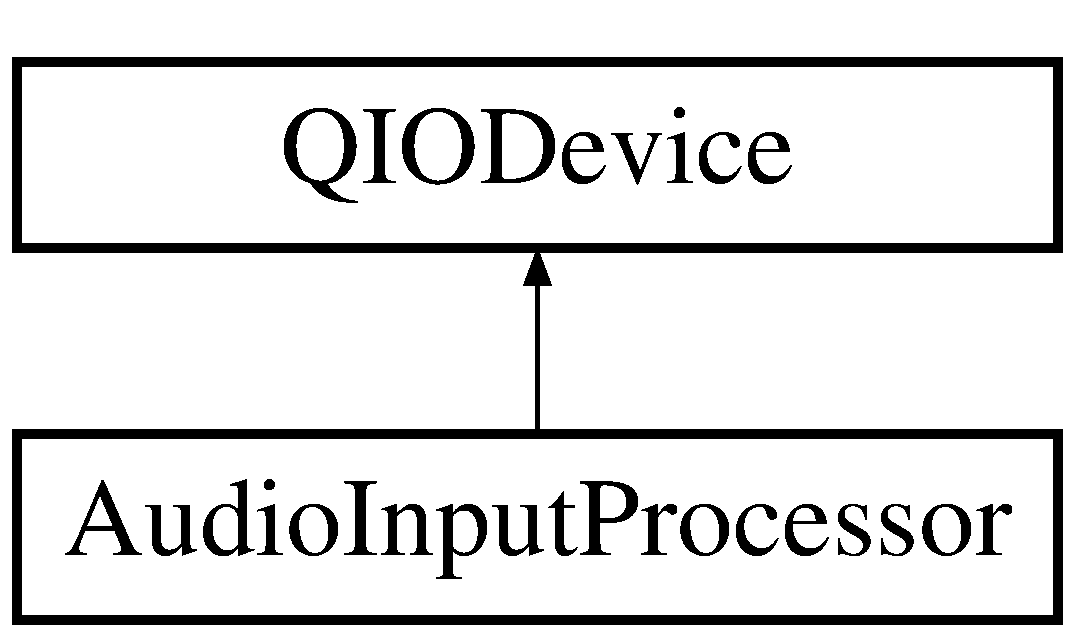
\includegraphics[height=2.000000cm]{classAudioInputProcessor}
\end{center}
\end{figure}
\subsection*{Signals}
\begin{DoxyCompactItemize}
\item 
\hypertarget{classAudioInputProcessor_af013a02bfef04a51fcab617633fb50ea}{void {\bfseries process\+Data} (Q\+Byte\+Array)}\label{classAudioInputProcessor_af013a02bfef04a51fcab617633fb50ea}

\end{DoxyCompactItemize}
\subsection*{Public Member Functions}
\begin{DoxyCompactItemize}
\item 
\hypertarget{classAudioInputProcessor_a4a53c5a1979a9d74ac58a834d3093ef9}{{\bfseries Audio\+Input\+Processor} (Q\+Object $\ast$parent=0)}\label{classAudioInputProcessor_a4a53c5a1979a9d74ac58a834d3093ef9}

\item 
\hypertarget{classAudioInputProcessor_a676d6ed660c621e1d3bf9700d757c688}{void {\bfseries start} ()}\label{classAudioInputProcessor_a676d6ed660c621e1d3bf9700d757c688}

\item 
\hypertarget{classAudioInputProcessor_a135b7ebe1b244ecec4751cd7f990172e}{const Q\+Audio\+Format {\bfseries format} () const }\label{classAudioInputProcessor_a135b7ebe1b244ecec4751cd7f990172e}

\end{DoxyCompactItemize}
\subsection*{Protected Member Functions}
\begin{DoxyCompactItemize}
\item 
\hypertarget{classAudioInputProcessor_a4ebabb98105dfb9bdd0192f09b8d82cc}{virtual qint64 {\bfseries read\+Data} (char $\ast$data, qint64 maxlen)}\label{classAudioInputProcessor_a4ebabb98105dfb9bdd0192f09b8d82cc}

\item 
\hypertarget{classAudioInputProcessor_a7e490a617e2f184e971d9c7c9633042e}{virtual qint64 {\bfseries write\+Data} (const char $\ast$data, qint64 len)}\label{classAudioInputProcessor_a7e490a617e2f184e971d9c7c9633042e}

\end{DoxyCompactItemize}


The documentation for this class was generated from the following files\+:\begin{DoxyCompactItemize}
\item 
src/Audio\+Input\+Processor.\+hpp\item 
src/Audio\+Input\+Processor.\+cpp\end{DoxyCompactItemize}

\hypertarget{classAudioOutputProcessor}{\section{Audio\+Output\+Processor Class Reference}
\label{classAudioOutputProcessor}\index{Audio\+Output\+Processor@{Audio\+Output\+Processor}}
}
Inheritance diagram for Audio\+Output\+Processor\+:\begin{figure}[H]
\begin{center}
\leavevmode
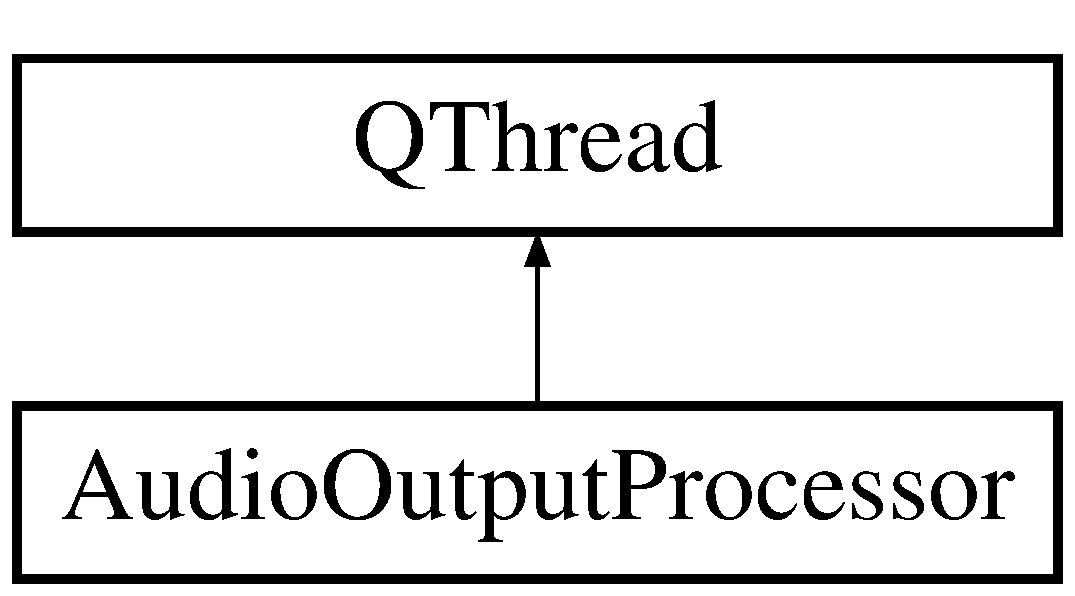
\includegraphics[height=2.000000cm]{classAudioOutputProcessor}
\end{center}
\end{figure}
\subsection*{Signals}
\begin{DoxyCompactItemize}
\item 
\hypertarget{classAudioOutputProcessor_ac5b95db59cbdb8d60f832653ae0a9793}{void {\bfseries stop\+Writing} ()}\label{classAudioOutputProcessor_ac5b95db59cbdb8d60f832653ae0a9793}

\item 
\hypertarget{classAudioOutputProcessor_a668b50fd985816d2d8a33f8546d72f42}{void {\bfseries start\+Writing} ()}\label{classAudioOutputProcessor_a668b50fd985816d2d8a33f8546d72f42}

\item 
\hypertarget{classAudioOutputProcessor_a763c98fb236616cd3b5d620dcf2e8a26}{void {\bfseries post\+Write\+To\+Device} ()}\label{classAudioOutputProcessor_a763c98fb236616cd3b5d620dcf2e8a26}

\end{DoxyCompactItemize}
\subsection*{Public Member Functions}
\begin{DoxyCompactItemize}
\item 
\hypertarget{classAudioOutputProcessor_ac345d660fcd1556450464f74973a8899}{{\bfseries Audio\+Output\+Processor} (Q\+Object $\ast$parent=0)}\label{classAudioOutputProcessor_ac345d660fcd1556450464f74973a8899}

\item 
\hypertarget{classAudioOutputProcessor_a3b5cb028b28051a7840cfe348683b472}{bool {\bfseries write} (const char $\ast$data, qint64 len)}\label{classAudioOutputProcessor_a3b5cb028b28051a7840cfe348683b472}

\end{DoxyCompactItemize}


The documentation for this class was generated from the following files\+:\begin{DoxyCompactItemize}
\item 
src/Audio\+Output\+Processor.\+hpp\item 
src/Audio\+Output\+Processor.\+cpp\end{DoxyCompactItemize}

\hypertarget{classAudioProcessorInstance}{\section{Audio\+Processor\+Instance Class Reference}
\label{classAudioProcessorInstance}\index{Audio\+Processor\+Instance@{Audio\+Processor\+Instance}}
}
Inheritance diagram for Audio\+Processor\+Instance\+:\begin{figure}[H]
\begin{center}
\leavevmode
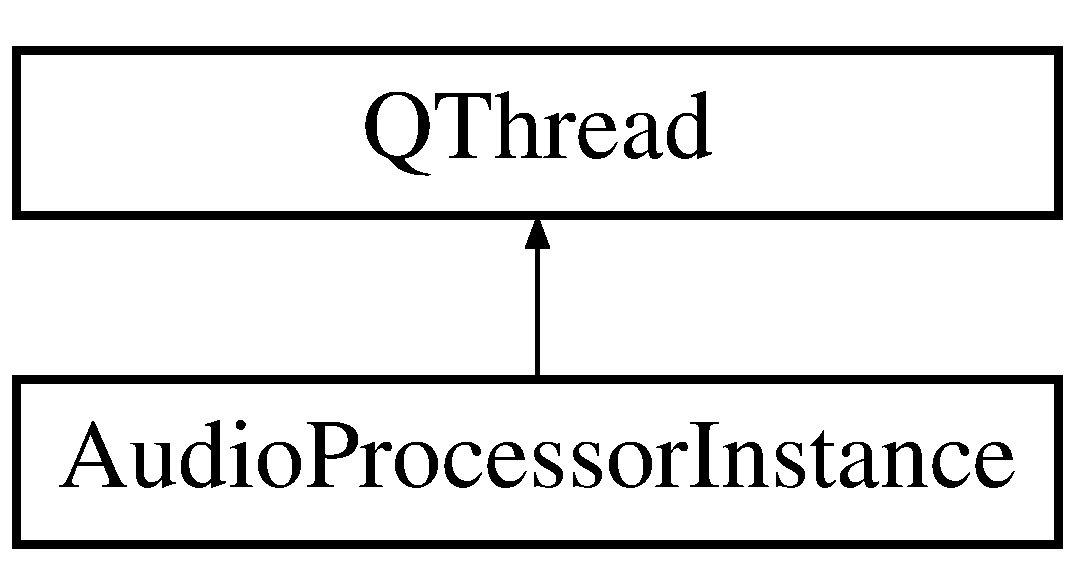
\includegraphics[height=2.000000cm]{classAudioProcessorInstance}
\end{center}
\end{figure}
\subsection*{Public Slots}
\begin{DoxyCompactItemize}
\item 
\hypertarget{classAudioProcessorInstance_a189a8cfa80d80c59179ea7f0ba6aa25d}{void {\bfseries write} ()}\label{classAudioProcessorInstance_a189a8cfa80d80c59179ea7f0ba6aa25d}

\end{DoxyCompactItemize}
\subsection*{Signals}
\begin{DoxyCompactItemize}
\item 
\hypertarget{classAudioProcessorInstance_a5c75fa4f596fc9e0b8fd049394b99fff}{void {\bfseries start\+Writing} ()}\label{classAudioProcessorInstance_a5c75fa4f596fc9e0b8fd049394b99fff}

\end{DoxyCompactItemize}
\subsection*{Public Member Functions}
\begin{DoxyCompactItemize}
\item 
\hypertarget{classAudioProcessorInstance_a1c8bfccd3b95be0b6d8e65595a5ce794}{{\bfseries Audio\+Processor\+Instance} (Q\+Object $\ast$parent=0)}\label{classAudioProcessorInstance_a1c8bfccd3b95be0b6d8e65595a5ce794}

\item 
\hypertarget{classAudioProcessorInstance_a560cd34c16cf1254f88647dceba53e42}{virtual void {\bfseries run} () Q\+\_\+\+D\+E\+C\+L\+\_\+\+O\+V\+E\+R\+R\+I\+D\+E}\label{classAudioProcessorInstance_a560cd34c16cf1254f88647dceba53e42}

\end{DoxyCompactItemize}


The documentation for this class was generated from the following file\+:\begin{DoxyCompactItemize}
\item 
src/Audio\+Test.\+hpp\end{DoxyCompactItemize}

\hypertarget{classBackend}{\section{Backend Class Reference}
\label{classBackend}\index{Backend@{Backend}}
}


The \hyperlink{classBackend}{Backend} class.  




{\ttfamily \#include $<$Backend.\+hpp$>$}

Inheritance diagram for Backend\+:\begin{figure}[H]
\begin{center}
\leavevmode
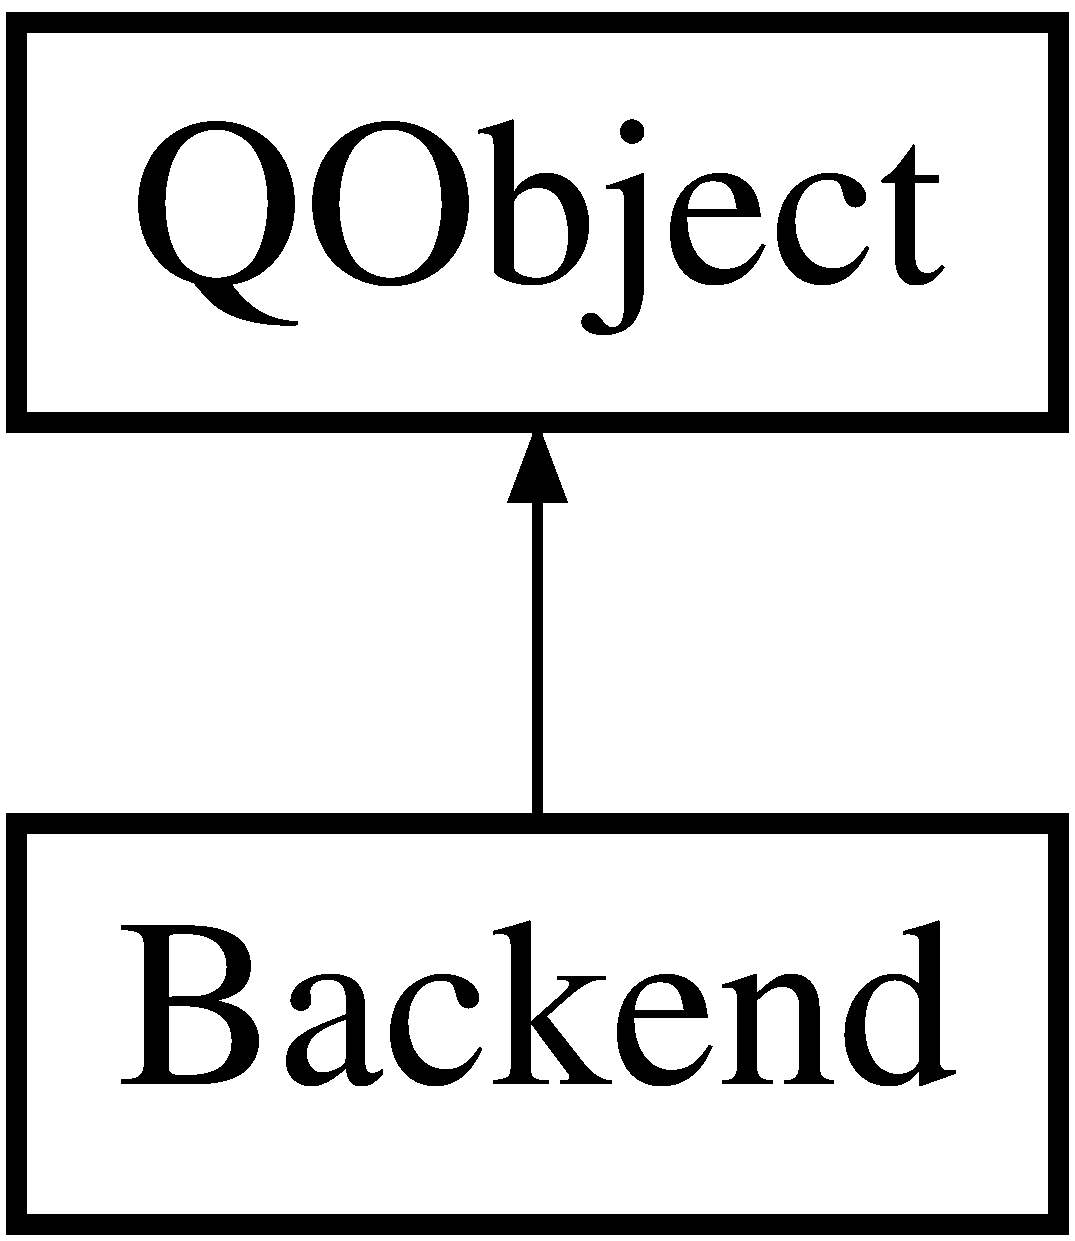
\includegraphics[height=2.000000cm]{classBackend}
\end{center}
\end{figure}
\subsection*{Public Slots}
\begin{DoxyCompactItemize}
\item 
void \hyperlink{classBackend_a0e96629d0e42a7a77ac25d83efe7b71f}{settings\+Window\+Requested} (\hyperlink{classInstances_1_1IInstance}{I\+Instance} $\ast$)
\begin{DoxyCompactList}\small\item\em \hyperlink{classBackend_a0e96629d0e42a7a77ac25d83efe7b71f}{Backend\+::settings\+Window\+Requested}. \end{DoxyCompactList}\item 
void \hyperlink{classBackend_a4208d788a7fc7ab5fea1e0ea5c349c99}{open\+Help} (\hyperlink{classInstances_1_1IInstance}{I\+Instance} $\ast$)
\begin{DoxyCompactList}\small\item\em \hyperlink{classBackend_a4208d788a7fc7ab5fea1e0ea5c349c99}{Backend\+::open\+Help}. \end{DoxyCompactList}\item 
void \hyperlink{classBackend_a502fcffad9e9435cdc43b7027df6b5a2}{instance\+Closing} (\hyperlink{classInstances_1_1IInstance}{I\+Instance} $\ast$)
\begin{DoxyCompactList}\small\item\em \hyperlink{classBackend_a502fcffad9e9435cdc43b7027df6b5a2}{Backend\+::instance\+Closing}. \end{DoxyCompactList}\item 
void \hyperlink{classBackend_af6c0389fd5ae6d4be1cdf4aa4bcbe2e9}{instance\+Destroyed} (Q\+Object $\ast$)
\begin{DoxyCompactList}\small\item\em \hyperlink{classBackend_af6c0389fd5ae6d4be1cdf4aa4bcbe2e9}{Backend\+::instance\+Destroyed}. \end{DoxyCompactList}\item 
void \hyperlink{classBackend_a18b602a36f6984e5494524be87d8e375}{instance\+Run\+Code} (\hyperlink{classInstances_1_1IInstance}{I\+Instance} $\ast$)
\begin{DoxyCompactList}\small\item\em \hyperlink{classBackend_a18b602a36f6984e5494524be87d8e375}{Backend\+::instance\+Run\+Code}. \end{DoxyCompactList}\item 
void \hyperlink{classBackend_a4baaa487c95ef37472f0ec0aa7b9e682}{instance\+Stop\+Code} (\hyperlink{classInstances_1_1IInstance}{I\+Instance} $\ast$)
\begin{DoxyCompactList}\small\item\em \hyperlink{classBackend_a4baaa487c95ef37472f0ec0aa7b9e682}{Backend\+::instance\+Stop\+Code}. \end{DoxyCompactList}\item 
void \hyperlink{classBackend_a76805ab500231fb990481d14a6e92fa6}{instance\+Changed\+Setting} (\hyperlink{classInstances_1_1IInstance}{I\+Instance} $\ast$, const Q\+String \&key, const Q\+Variant \&value)
\begin{DoxyCompactList}\small\item\em \hyperlink{classBackend_a76805ab500231fb990481d14a6e92fa6}{Backend\+::instance\+Changed\+Setting}. \end{DoxyCompactList}\item 
void \hyperlink{classBackend_a59f35222ca04fc4b47bfcebf1d00e43c}{instance\+Request\+Setting} (\hyperlink{classInstances_1_1IInstance}{I\+Instance} $\ast$, const Q\+String \&key, Q\+Variant \&value)
\begin{DoxyCompactList}\small\item\em \hyperlink{classBackend_a59f35222ca04fc4b47bfcebf1d00e43c}{Backend\+::instance\+Request\+Setting}. \end{DoxyCompactList}\item 
void \hyperlink{classBackend_a05a0cec3dde03eaac9d4007d9d43e69e}{instance\+Changed\+Settings} (\hyperlink{classInstances_1_1IInstance}{I\+Instance} $\ast$, const Q\+Hash$<$ Q\+String, Q\+Variant $>$ \&)
\begin{DoxyCompactList}\small\item\em \hyperlink{classBackend_a05a0cec3dde03eaac9d4007d9d43e69e}{Backend\+::instance\+Changed\+Settings}. \end{DoxyCompactList}\item 
void \hyperlink{classBackend_ab300ebcb08269780d5aca31d4e2e7f96}{instance\+Request\+Settings} (\hyperlink{classInstances_1_1IInstance}{I\+Instance} $\ast$, Q\+Hash$<$ Q\+String, Q\+Variant $>$ \&)
\begin{DoxyCompactList}\small\item\em \hyperlink{classBackend_ab300ebcb08269780d5aca31d4e2e7f96}{Backend\+::instance\+Request\+Settings}. \end{DoxyCompactList}\item 
void \hyperlink{classBackend_aa0c4137f5da3c1cb512b4c2bd65ebe34}{child\+Said\+Close\+All} ()
\begin{DoxyCompactList}\small\item\em \hyperlink{classBackend_aa0c4137f5da3c1cb512b4c2bd65ebe34}{Backend\+::child\+Said\+Close\+All}. \end{DoxyCompactList}\item 
void \hyperlink{classBackend_a470ae474cf3d91ad5639906bf0786f99}{get\+Execution\+Results} (\hyperlink{classQtSoundThread}{Qt\+Sound\+Thread} $\ast$, Q\+String)
\begin{DoxyCompactList}\small\item\em \hyperlink{classBackend_a470ae474cf3d91ad5639906bf0786f99}{Backend\+::get\+Execution\+Results}. \end{DoxyCompactList}\item 
\hypertarget{classBackend_ac1015a3827ecb51a218bd7407c25e404}{void {\bfseries get\+Execution\+Results} (\hyperlink{classPySoundThread}{Py\+Sound\+Thread} $\ast$, Q\+String, int)}\label{classBackend_ac1015a3827ecb51a218bd7407c25e404}

\item 
\hypertarget{classBackend_a003d57ff15a365ce17c5f9aad70f80cf}{void {\bfseries get\+Execution\+Results} (\hyperlink{classPyLiveThread}{Py\+Live\+Thread} $\ast$, Q\+String, int)}\label{classBackend_a003d57ff15a365ce17c5f9aad70f80cf}

\item 
\hypertarget{classBackend_af71ab9234eada09c515370fe68a2a60c}{void {\bfseries get\+Execution\+Results} (\hyperlink{classGlLiveThread}{Gl\+Live\+Thread} $\ast$, Q\+String)}\label{classBackend_af71ab9234eada09c515370fe68a2a60c}

\item 
\hypertarget{classBackend_ac773069daf1253e45cf1bac598ea07e5}{void {\bfseries get\+Error} (\hyperlink{classGlLiveThread}{Gl\+Live\+Thread} $\ast$, Q\+String, int)}\label{classBackend_ac773069daf1253e45cf1bac598ea07e5}

\end{DoxyCompactItemize}
\subsection*{Signals}
\begin{DoxyCompactItemize}
\item 
\hypertarget{classBackend_a2ac57980d074469c38e7f440010e4902}{void {\bfseries warning\+Signal} (Q\+Widget $\ast$, Q\+String)}\label{classBackend_a2ac57980d074469c38e7f440010e4902}

\item 
\hypertarget{classBackend_a6087c09506cdc2de62e71e07c848f6a4}{void {\bfseries close\+Action} ()}\label{classBackend_a6087c09506cdc2de62e71e07c848f6a4}

\item 
\hypertarget{classBackend_a1442023af58aa9d10895e544612bb148}{void {\bfseries save\+Action} ()}\label{classBackend_a1442023af58aa9d10895e544612bb148}

\item 
\hypertarget{classBackend_ac983ee553561b1fc8f7d6b811c5caefd}{void {\bfseries show\+Results} (const Q\+String \&)}\label{classBackend_ac983ee553561b1fc8f7d6b811c5caefd}

\item 
\hypertarget{classBackend_a9bb0c4a9fc2f93ff78468c60f2d64329}{void {\bfseries child\+Do\+Save\+Settings} ()}\label{classBackend_a9bb0c4a9fc2f93ff78468c60f2d64329}

\end{DoxyCompactItemize}
\subsection*{Public Member Functions}
\begin{DoxyCompactItemize}
\item 
\hyperlink{classBackend_a57e21c0be0119a102f8ae27db6ac3106}{Backend} (Q\+Object $\ast$parent=0)
\begin{DoxyCompactList}\small\item\em \hyperlink{classBackend_a57e21c0be0119a102f8ae27db6ac3106}{Backend\+::\+Backend}. \end{DoxyCompactList}\item 
\hyperlink{classBackend_ad4a4bc528854a918880d5e6b5de05cc6}{$\sim$\+Backend} ()
\begin{DoxyCompactList}\small\item\em \hyperlink{classBackend_ad4a4bc528854a918880d5e6b5de05cc6}{Backend\+::$\sim$\+Backend}. \end{DoxyCompactList}\item 
void \hyperlink{classBackend_af5d23c3090d7b3643ed0df364ddfb70c}{add\+Instance} (\hyperlink{classInstances_1_1IInstance}{I\+Instance} $\ast$, bool=true)
\begin{DoxyCompactList}\small\item\em Backend\+::add\+Child. \end{DoxyCompactList}\item 
\hypertarget{classBackend_af3add13d84efb30e198cd6ce08204696}{void {\bfseries create\+Child} ()}\label{classBackend_af3add13d84efb30e198cd6ce08204696}

\item 
void \hyperlink{classBackend_a85c891e4026d4597adb6462488be3d2e}{child\+Exited} (\hyperlink{classInstances_1_1IInstance}{I\+Instance} $\ast$, Q\+String)
\begin{DoxyCompactList}\small\item\em \hyperlink{classBackend_a85c891e4026d4597adb6462488be3d2e}{Backend\+::child\+Exited}. \end{DoxyCompactList}\item 
bool \hyperlink{classBackend_a648433115e8e2a94e9084628f408465a}{is\+Last} ()
\begin{DoxyCompactList}\small\item\em \hyperlink{classBackend_a648433115e8e2a94e9084628f408465a}{Backend\+::is\+Last}. \end{DoxyCompactList}\item 
bool \hyperlink{classBackend_a390eb82dfe8025c1f31ddacc8a25f801}{remove\+Instance} (\hyperlink{classInstances_1_1IInstance}{I\+Instance} $\ast$, bool=true)
\begin{DoxyCompactList}\small\item\em Backend\+::remove\+Child. \end{DoxyCompactList}\item 
\hypertarget{classBackend_af8ce743855e7241ebf43d2c7527d9a72}{bool {\bfseries remove\+Instance} (int, bool=true)}\label{classBackend_af8ce743855e7241ebf43d2c7527d9a72}

\item 
void \hyperlink{classBackend_afcbcbf35d3678dc95de1acee4a8b4307}{remove\+Settings} (\hyperlink{classInstances_1_1IInstance}{I\+Instance} $\ast$)
\begin{DoxyCompactList}\small\item\em \hyperlink{classBackend_afcbcbf35d3678dc95de1acee4a8b4307}{Backend\+::remove\+Settings}. \end{DoxyCompactList}\item 
\hypertarget{classBackend_a1681e99e726bde1078b2f923344d6c19}{void {\bfseries remove\+Settings} (int)}\label{classBackend_a1681e99e726bde1078b2f923344d6c19}

\item 
\hypertarget{classBackend_a393c2f03c7b2842a2f33af1d37936a8b}{void {\bfseries save\+All\+Settings} ()}\label{classBackend_a393c2f03c7b2842a2f33af1d37936a8b}

\item 
\hypertarget{classBackend_a103ebcb39d6c6857a10975cb8f135f89}{void {\bfseries save\+Settings} (\hyperlink{classInstances_1_1IInstance}{I\+Instance} $\ast$, Q\+String)}\label{classBackend_a103ebcb39d6c6857a10975cb8f135f89}

\item 
Q\+Hash$<$ Q\+String, Q\+Variant $>$ \hyperlink{classBackend_afb078e1c344aef87c53c079411003536}{get\+Settings} (\hyperlink{classInstances_1_1IInstance}{I\+Instance} $\ast$)
\begin{DoxyCompactList}\small\item\em \hyperlink{classBackend_afb078e1c344aef87c53c079411003536}{Backend\+::get\+Settings}. \end{DoxyCompactList}\item 
Q\+Hash$<$ Q\+String, Q\+Variant $>$ \hyperlink{classBackend_a57e1f06d09bb993d693c2287c0f8e525}{get\+Settings} (int id)
\begin{DoxyCompactList}\small\item\em \hyperlink{classBackend_afb078e1c344aef87c53c079411003536}{Backend\+::get\+Settings}. \end{DoxyCompactList}\item 
int \hyperlink{classBackend_a32ac5490f4f303e2a14ffdf3788f347d}{next\+I\+D} ()
\begin{DoxyCompactList}\small\item\em \hyperlink{classBackend_a32ac5490f4f303e2a14ffdf3788f347d}{Backend\+::next\+I\+D}. \end{DoxyCompactList}\item 
Q\+List$<$ int $>$ \hyperlink{classBackend_a2a77d2660fe12daa1d277181efbfb110}{load\+Ids} ()
\begin{DoxyCompactList}\small\item\em \hyperlink{classBackend_a2a77d2660fe12daa1d277181efbfb110}{Backend\+::load\+Ids}. \end{DoxyCompactList}\item 
\hypertarget{classBackend_a49aa08ee70e290fddb85aef0f3fc5c66}{Q\+Variant {\bfseries get\+Setting} (Q\+String key, Q\+Variant default\+Value=Q\+Variant())}\label{classBackend_a49aa08ee70e290fddb85aef0f3fc5c66}

\end{DoxyCompactItemize}
\subsection*{Static Public Member Functions}
\begin{DoxyCompactItemize}
\item 
static Q\+Dir \hyperlink{classBackend_af319360536a63ebdfff12dee5e844eca}{directory\+Of} (const Q\+String \&)
\begin{DoxyCompactList}\small\item\em \hyperlink{classBackend_af319360536a63ebdfff12dee5e844eca}{Backend\+::directory\+Of}. \end{DoxyCompactList}\end{DoxyCompactItemize}


\subsection{Detailed Description}
The \hyperlink{classBackend}{Backend} class. 

The heart and soul of the eidtors functionality. Is connected to all the other parts of the application (through S\+I\+G\+N\+A\+Ls as well as references) and keeps track of all the windows and code evaluation threads that are created and deleted. 

\subsection{Constructor \& Destructor Documentation}
\hypertarget{classBackend_a57e21c0be0119a102f8ae27db6ac3106}{\index{Backend@{Backend}!Backend@{Backend}}
\index{Backend@{Backend}!Backend@{Backend}}
\subsubsection[{Backend}]{\setlength{\rightskip}{0pt plus 5cm}Backend\+::\+Backend (
\begin{DoxyParamCaption}
\item[{Q\+Object $\ast$}]{parent = {\ttfamily 0}}
\end{DoxyParamCaption}
)\hspace{0.3cm}{\ttfamily [explicit]}}}\label{classBackend_a57e21c0be0119a102f8ae27db6ac3106}


\hyperlink{classBackend_a57e21c0be0119a102f8ae27db6ac3106}{Backend\+::\+Backend}. 


\begin{DoxyParams}{Parameters}
{\em parent} & The constructor of the \hyperlink{classBackend}{Backend} class. Initializes the editor window list and the thread list as well as the settings backend. \\
\hline
\end{DoxyParams}


References Settings\+Backend\+::get\+Settings\+For().

\hypertarget{classBackend_ad4a4bc528854a918880d5e6b5de05cc6}{\index{Backend@{Backend}!````~Backend@{$\sim$\+Backend}}
\index{````~Backend@{$\sim$\+Backend}!Backend@{Backend}}
\subsubsection[{$\sim$\+Backend}]{\setlength{\rightskip}{0pt plus 5cm}Backend\+::$\sim$\+Backend (
\begin{DoxyParamCaption}
{}
\end{DoxyParamCaption}
)}}\label{classBackend_ad4a4bc528854a918880d5e6b5de05cc6}


\hyperlink{classBackend_ad4a4bc528854a918880d5e6b5de05cc6}{Backend\+::$\sim$\+Backend}. 

The destructor of the \hyperlink{classBackend}{Backend} class. Eliminates all the threads that were orphaned when all the windows closed. 

\subsection{Member Function Documentation}
\hypertarget{classBackend_af5d23c3090d7b3643ed0df364ddfb70c}{\index{Backend@{Backend}!add\+Instance@{add\+Instance}}
\index{add\+Instance@{add\+Instance}!Backend@{Backend}}
\subsubsection[{add\+Instance}]{\setlength{\rightskip}{0pt plus 5cm}void Backend\+::add\+Instance (
\begin{DoxyParamCaption}
\item[{{\bf I\+Instance} $\ast$}]{instance, }
\item[{bool}]{remove\+Settings = {\ttfamily true}}
\end{DoxyParamCaption}
)}}\label{classBackend_af5d23c3090d7b3643ed0df364ddfb70c}


Backend\+::add\+Child. 


\begin{DoxyParams}{Parameters}
{\em instance} & \\
\hline
{\em remove\+Settings} & Is called by one of the editor window instances; enlists the child and creates an empty thread entry in the list so that the two correlate. \\
\hline
\end{DoxyParams}


References child\+Said\+Close\+All(), get\+Settings(), instance\+Changed\+Setting(), instance\+Changed\+Settings(), instance\+Closing(), instance\+Destroyed(), instance\+Request\+Setting(), instance\+Request\+Settings(), instance\+Run\+Code(), instance\+Stop\+Code(), open\+Help(), Settings\+Backend\+::remove\+Settings(), and settings\+Window\+Requested().



Referenced by Boot\+Loader\+::accept\+Connection().

\hypertarget{classBackend_a85c891e4026d4597adb6462488be3d2e}{\index{Backend@{Backend}!child\+Exited@{child\+Exited}}
\index{child\+Exited@{child\+Exited}!Backend@{Backend}}
\subsubsection[{child\+Exited}]{\setlength{\rightskip}{0pt plus 5cm}void Backend\+::child\+Exited (
\begin{DoxyParamCaption}
\item[{{\bf I\+Instance} $\ast$}]{child, }
\item[{Q\+String}]{file}
\end{DoxyParamCaption}
)}}\label{classBackend_a85c891e4026d4597adb6462488be3d2e}


\hyperlink{classBackend_a85c891e4026d4597adb6462488be3d2e}{Backend\+::child\+Exited}. 


\begin{DoxyParams}{Parameters}
{\em child} & \\
\hline
{\em file} & Is called by one of the editor window instances; when the child reacts to the closed\+Action, it is removed from the list. \\
\hline
\end{DoxyParams}
\hypertarget{classBackend_aa0c4137f5da3c1cb512b4c2bd65ebe34}{\index{Backend@{Backend}!child\+Said\+Close\+All@{child\+Said\+Close\+All}}
\index{child\+Said\+Close\+All@{child\+Said\+Close\+All}!Backend@{Backend}}
\subsubsection[{child\+Said\+Close\+All}]{\setlength{\rightskip}{0pt plus 5cm}void Backend\+::child\+Said\+Close\+All (
\begin{DoxyParamCaption}
{}
\end{DoxyParamCaption}
)\hspace{0.3cm}{\ttfamily [slot]}}}\label{classBackend_aa0c4137f5da3c1cb512b4c2bd65ebe34}


\hyperlink{classBackend_aa0c4137f5da3c1cb512b4c2bd65ebe34}{Backend\+::child\+Said\+Close\+All}. 

Is called by one of the editor window instances; when a user requests to exit the application, this will tell all the children to terminate. 

References instance\+Destroyed(), remove\+Instance(), and Settings\+Backend\+::remove\+Settings().



Referenced by add\+Instance().

\hypertarget{classBackend_af319360536a63ebdfff12dee5e844eca}{\index{Backend@{Backend}!directory\+Of@{directory\+Of}}
\index{directory\+Of@{directory\+Of}!Backend@{Backend}}
\subsubsection[{directory\+Of}]{\setlength{\rightskip}{0pt plus 5cm}Q\+Dir Backend\+::directory\+Of (
\begin{DoxyParamCaption}
\item[{const Q\+String \&}]{subdir}
\end{DoxyParamCaption}
)\hspace{0.3cm}{\ttfamily [static]}}}\label{classBackend_af319360536a63ebdfff12dee5e844eca}


\hyperlink{classBackend_af319360536a63ebdfff12dee5e844eca}{Backend\+::directory\+Of}. 


\begin{DoxyParams}{Parameters}
{\em subdir} & \\
\hline
\end{DoxyParams}
\begin{DoxyReturn}{Returns}
the directory one wants to navigate into
\end{DoxyReturn}
Platform independent wrapper to changing the directory. 

Referenced by open\+Help().

\hypertarget{classBackend_a470ae474cf3d91ad5639906bf0786f99}{\index{Backend@{Backend}!get\+Execution\+Results@{get\+Execution\+Results}}
\index{get\+Execution\+Results@{get\+Execution\+Results}!Backend@{Backend}}
\subsubsection[{get\+Execution\+Results}]{\setlength{\rightskip}{0pt plus 5cm}void Backend\+::get\+Execution\+Results (
\begin{DoxyParamCaption}
\item[{{\bf Qt\+Sound\+Thread} $\ast$}]{thread, }
\item[{Q\+String}]{returned\+Exception}
\end{DoxyParamCaption}
)\hspace{0.3cm}{\ttfamily [slot]}}}\label{classBackend_a470ae474cf3d91ad5639906bf0786f99}


\hyperlink{classBackend_a470ae474cf3d91ad5639906bf0786f99}{Backend\+::get\+Execution\+Results}. 

reacts to the done S\+I\+G\+N\+A\+L by terminating the thread and Q\+\_\+\+E\+M\+I\+Tting a show\+Results S\+I\+G\+N\+A\+L for the Q\+Widgets to display \hypertarget{classBackend_afb078e1c344aef87c53c079411003536}{\index{Backend@{Backend}!get\+Settings@{get\+Settings}}
\index{get\+Settings@{get\+Settings}!Backend@{Backend}}
\subsubsection[{get\+Settings}]{\setlength{\rightskip}{0pt plus 5cm}Q\+Hash$<$ Q\+String, Q\+Variant $>$ Backend\+::get\+Settings (
\begin{DoxyParamCaption}
\item[{{\bf I\+Instance} $\ast$}]{instance}
\end{DoxyParamCaption}
)}}\label{classBackend_afb078e1c344aef87c53c079411003536}


\hyperlink{classBackend_afb078e1c344aef87c53c079411003536}{Backend\+::get\+Settings}. 


\begin{DoxyParams}{Parameters}
{\em instance} & \\
\hline
\end{DoxyParams}
\begin{DoxyReturn}{Returns}
a list of current settings
\end{DoxyReturn}
Gets all settings for a specific window. 

Referenced by add\+Instance().

\hypertarget{classBackend_a57e1f06d09bb993d693c2287c0f8e525}{\index{Backend@{Backend}!get\+Settings@{get\+Settings}}
\index{get\+Settings@{get\+Settings}!Backend@{Backend}}
\subsubsection[{get\+Settings}]{\setlength{\rightskip}{0pt plus 5cm}Q\+Hash$<$ Q\+String, Q\+Variant $>$ Backend\+::get\+Settings (
\begin{DoxyParamCaption}
\item[{int}]{id}
\end{DoxyParamCaption}
)}}\label{classBackend_a57e1f06d09bb993d693c2287c0f8e525}


\hyperlink{classBackend_afb078e1c344aef87c53c079411003536}{Backend\+::get\+Settings}. 


\begin{DoxyParams}{Parameters}
{\em id} & \\
\hline
\end{DoxyParams}
\begin{DoxyReturn}{Returns}
a Q\+Hash of all the settings for an id.
\end{DoxyReturn}
looks up the settings for an editor window child. 

References Settings\+Backend\+::get\+Settings().

\hypertarget{classBackend_a76805ab500231fb990481d14a6e92fa6}{\index{Backend@{Backend}!instance\+Changed\+Setting@{instance\+Changed\+Setting}}
\index{instance\+Changed\+Setting@{instance\+Changed\+Setting}!Backend@{Backend}}
\subsubsection[{instance\+Changed\+Setting}]{\setlength{\rightskip}{0pt plus 5cm}void Backend\+::instance\+Changed\+Setting (
\begin{DoxyParamCaption}
\item[{{\bf I\+Instance} $\ast$}]{instance, }
\item[{const Q\+String \&}]{key, }
\item[{const Q\+Variant \&}]{value}
\end{DoxyParamCaption}
)\hspace{0.3cm}{\ttfamily [slot]}}}\label{classBackend_a76805ab500231fb990481d14a6e92fa6}


\hyperlink{classBackend_a76805ab500231fb990481d14a6e92fa6}{Backend\+::instance\+Changed\+Setting}. 


\begin{DoxyParams}{Parameters}
{\em instance} & \\
\hline
{\em key} & \\
\hline
{\em value} & Reacts to the instance changing settings. Saves the new settings. \\
\hline
\end{DoxyParams}


References Settings\+Backend\+::save\+Settings\+For().



Referenced by add\+Instance().

\hypertarget{classBackend_a05a0cec3dde03eaac9d4007d9d43e69e}{\index{Backend@{Backend}!instance\+Changed\+Settings@{instance\+Changed\+Settings}}
\index{instance\+Changed\+Settings@{instance\+Changed\+Settings}!Backend@{Backend}}
\subsubsection[{instance\+Changed\+Settings}]{\setlength{\rightskip}{0pt plus 5cm}void Backend\+::instance\+Changed\+Settings (
\begin{DoxyParamCaption}
\item[{{\bf I\+Instance} $\ast$}]{instance, }
\item[{const Q\+Hash$<$ Q\+String, Q\+Variant $>$ \&}]{set}
\end{DoxyParamCaption}
)\hspace{0.3cm}{\ttfamily [slot]}}}\label{classBackend_a05a0cec3dde03eaac9d4007d9d43e69e}


\hyperlink{classBackend_a05a0cec3dde03eaac9d4007d9d43e69e}{Backend\+::instance\+Changed\+Settings}. 


\begin{DoxyParams}{Parameters}
{\em instance} & \\
\hline
{\em set} & Reacts to the instance changing its settings(as a set). Saves the new settings. T\+O\+D\+O\+: Needed(overloaded call)? \\
\hline
\end{DoxyParams}


References Settings\+Backend\+::save\+Settings\+For().



Referenced by add\+Instance().

\hypertarget{classBackend_a502fcffad9e9435cdc43b7027df6b5a2}{\index{Backend@{Backend}!instance\+Closing@{instance\+Closing}}
\index{instance\+Closing@{instance\+Closing}!Backend@{Backend}}
\subsubsection[{instance\+Closing}]{\setlength{\rightskip}{0pt plus 5cm}void Backend\+::instance\+Closing (
\begin{DoxyParamCaption}
\item[{{\bf I\+Instance} $\ast$}]{instance}
\end{DoxyParamCaption}
)\hspace{0.3cm}{\ttfamily [slot]}}}\label{classBackend_a502fcffad9e9435cdc43b7027df6b5a2}


\hyperlink{classBackend_a502fcffad9e9435cdc43b7027df6b5a2}{Backend\+::instance\+Closing}. 


\begin{DoxyParams}{Parameters}
{\em instance} & Reacts to the closing signal and calls the \hyperlink{classBackend_a390eb82dfe8025c1f31ddacc8a25f801}{remove\+Instance()} routine. T\+O\+D\+O\+: Needed? \\
\hline
\end{DoxyParams}


References remove\+Instance().



Referenced by add\+Instance().

\hypertarget{classBackend_af6c0389fd5ae6d4be1cdf4aa4bcbe2e9}{\index{Backend@{Backend}!instance\+Destroyed@{instance\+Destroyed}}
\index{instance\+Destroyed@{instance\+Destroyed}!Backend@{Backend}}
\subsubsection[{instance\+Destroyed}]{\setlength{\rightskip}{0pt plus 5cm}void Backend\+::instance\+Destroyed (
\begin{DoxyParamCaption}
\item[{Q\+Object $\ast$}]{instance}
\end{DoxyParamCaption}
)\hspace{0.3cm}{\ttfamily [slot]}}}\label{classBackend_af6c0389fd5ae6d4be1cdf4aa4bcbe2e9}


\hyperlink{classBackend_af6c0389fd5ae6d4be1cdf4aa4bcbe2e9}{Backend\+::instance\+Destroyed}. 


\begin{DoxyParams}{Parameters}
{\em instance} & Reacts to the destroyed signal and removes the instance from the backends' memory. \\
\hline
\end{DoxyParams}


References remove\+Instance().



Referenced by add\+Instance(), and child\+Said\+Close\+All().

\hypertarget{classBackend_a59f35222ca04fc4b47bfcebf1d00e43c}{\index{Backend@{Backend}!instance\+Request\+Setting@{instance\+Request\+Setting}}
\index{instance\+Request\+Setting@{instance\+Request\+Setting}!Backend@{Backend}}
\subsubsection[{instance\+Request\+Setting}]{\setlength{\rightskip}{0pt plus 5cm}void Backend\+::instance\+Request\+Setting (
\begin{DoxyParamCaption}
\item[{{\bf I\+Instance} $\ast$}]{instance, }
\item[{const Q\+String \&}]{key, }
\item[{Q\+Variant \&}]{value}
\end{DoxyParamCaption}
)\hspace{0.3cm}{\ttfamily [slot]}}}\label{classBackend_a59f35222ca04fc4b47bfcebf1d00e43c}


\hyperlink{classBackend_a59f35222ca04fc4b47bfcebf1d00e43c}{Backend\+::instance\+Request\+Setting}. 


\begin{DoxyParams}{Parameters}
{\em instance} & \\
\hline
{\em key} & \\
\hline
{\em value} & Reacts to the instance requesting its settings for a given key. \\
\hline
\end{DoxyParams}


References Settings\+Backend\+::get\+Settings\+For().



Referenced by add\+Instance().

\hypertarget{classBackend_ab300ebcb08269780d5aca31d4e2e7f96}{\index{Backend@{Backend}!instance\+Request\+Settings@{instance\+Request\+Settings}}
\index{instance\+Request\+Settings@{instance\+Request\+Settings}!Backend@{Backend}}
\subsubsection[{instance\+Request\+Settings}]{\setlength{\rightskip}{0pt plus 5cm}void Backend\+::instance\+Request\+Settings (
\begin{DoxyParamCaption}
\item[{{\bf I\+Instance} $\ast$}]{instance, }
\item[{Q\+Hash$<$ Q\+String, Q\+Variant $>$ \&}]{set}
\end{DoxyParamCaption}
)\hspace{0.3cm}{\ttfamily [slot]}}}\label{classBackend_ab300ebcb08269780d5aca31d4e2e7f96}


\hyperlink{classBackend_ab300ebcb08269780d5aca31d4e2e7f96}{Backend\+::instance\+Request\+Settings}. 


\begin{DoxyParams}{Parameters}
{\em instance} & \\
\hline
{\em set} & T\+O\+D\+O\+: Needed(overloaded call)? \\
\hline
\end{DoxyParams}


References Settings\+Backend\+::get\+Settings().



Referenced by add\+Instance().

\hypertarget{classBackend_a18b602a36f6984e5494524be87d8e375}{\index{Backend@{Backend}!instance\+Run\+Code@{instance\+Run\+Code}}
\index{instance\+Run\+Code@{instance\+Run\+Code}!Backend@{Backend}}
\subsubsection[{instance\+Run\+Code}]{\setlength{\rightskip}{0pt plus 5cm}void Backend\+::instance\+Run\+Code (
\begin{DoxyParamCaption}
\item[{{\bf I\+Instance} $\ast$}]{instance}
\end{DoxyParamCaption}
)\hspace{0.3cm}{\ttfamily [slot]}}}\label{classBackend_a18b602a36f6984e5494524be87d8e375}


\hyperlink{classBackend_a18b602a36f6984e5494524be87d8e375}{Backend\+::instance\+Run\+Code}. 

reacts to the run S\+I\+G\+N\+A\+L by running the code(duh) that is in the editor at the moment. 

References Settings\+Backend\+::get\+Settings\+For().



Referenced by add\+Instance().

\hypertarget{classBackend_a4baaa487c95ef37472f0ec0aa7b9e682}{\index{Backend@{Backend}!instance\+Stop\+Code@{instance\+Stop\+Code}}
\index{instance\+Stop\+Code@{instance\+Stop\+Code}!Backend@{Backend}}
\subsubsection[{instance\+Stop\+Code}]{\setlength{\rightskip}{0pt plus 5cm}void Backend\+::instance\+Stop\+Code (
\begin{DoxyParamCaption}
\item[{{\bf I\+Instance} $\ast$}]{instance}
\end{DoxyParamCaption}
)\hspace{0.3cm}{\ttfamily [slot]}}}\label{classBackend_a4baaa487c95ef37472f0ec0aa7b9e682}


\hyperlink{classBackend_a4baaa487c95ef37472f0ec0aa7b9e682}{Backend\+::instance\+Stop\+Code}. 


\begin{DoxyParams}{Parameters}
{\em instance} & Reacts to the stop\+Code signal of an instance. Stops the executing context. \\
\hline
\end{DoxyParams}


Referenced by add\+Instance().

\hypertarget{classBackend_a648433115e8e2a94e9084628f408465a}{\index{Backend@{Backend}!is\+Last@{is\+Last}}
\index{is\+Last@{is\+Last}!Backend@{Backend}}
\subsubsection[{is\+Last}]{\setlength{\rightskip}{0pt plus 5cm}bool Backend\+::is\+Last (
\begin{DoxyParamCaption}
{}
\end{DoxyParamCaption}
)}}\label{classBackend_a648433115e8e2a94e9084628f408465a}


\hyperlink{classBackend_a648433115e8e2a94e9084628f408465a}{Backend\+::is\+Last}. 

\begin{DoxyReturn}{Returns}
true if the child is the last one, false otherwise
\end{DoxyReturn}
checks whether there is only one or no child in the list. \hypertarget{classBackend_a2a77d2660fe12daa1d277181efbfb110}{\index{Backend@{Backend}!load\+Ids@{load\+Ids}}
\index{load\+Ids@{load\+Ids}!Backend@{Backend}}
\subsubsection[{load\+Ids}]{\setlength{\rightskip}{0pt plus 5cm}Q\+List$<$ int $>$ Backend\+::load\+Ids (
\begin{DoxyParamCaption}
{}
\end{DoxyParamCaption}
)}}\label{classBackend_a2a77d2660fe12daa1d277181efbfb110}


\hyperlink{classBackend_a2a77d2660fe12daa1d277181efbfb110}{Backend\+::load\+Ids}. 

\begin{DoxyReturn}{Returns}
A list of used I\+Ds
\end{DoxyReturn}
Return the list of ids for which settings should exist. 

References Settings\+Backend\+::get\+Settings\+For().

\hypertarget{classBackend_a32ac5490f4f303e2a14ffdf3788f347d}{\index{Backend@{Backend}!next\+I\+D@{next\+I\+D}}
\index{next\+I\+D@{next\+I\+D}!Backend@{Backend}}
\subsubsection[{next\+I\+D}]{\setlength{\rightskip}{0pt plus 5cm}int Backend\+::next\+I\+D (
\begin{DoxyParamCaption}
{}
\end{DoxyParamCaption}
)}}\label{classBackend_a32ac5490f4f303e2a14ffdf3788f347d}


\hyperlink{classBackend_a32ac5490f4f303e2a14ffdf3788f347d}{Backend\+::next\+I\+D}. 

\begin{DoxyReturn}{Returns}
Free to use id
\end{DoxyReturn}
Look up the first free I\+D for a new Instance. 

Referenced by Boot\+Loader\+::accept\+Connection().

\hypertarget{classBackend_a4208d788a7fc7ab5fea1e0ea5c349c99}{\index{Backend@{Backend}!open\+Help@{open\+Help}}
\index{open\+Help@{open\+Help}!Backend@{Backend}}
\subsubsection[{open\+Help}]{\setlength{\rightskip}{0pt plus 5cm}void Backend\+::open\+Help (
\begin{DoxyParamCaption}
\item[{{\bf I\+Instance} $\ast$}]{}
\end{DoxyParamCaption}
)\hspace{0.3cm}{\ttfamily [slot]}}}\label{classBackend_a4208d788a7fc7ab5fea1e0ea5c349c99}


\hyperlink{classBackend_a4208d788a7fc7ab5fea1e0ea5c349c99}{Backend\+::open\+Help}. 

Opens a help window in H\+T\+M\+L. 

References directory\+Of().



Referenced by add\+Instance().

\hypertarget{classBackend_a390eb82dfe8025c1f31ddacc8a25f801}{\index{Backend@{Backend}!remove\+Instance@{remove\+Instance}}
\index{remove\+Instance@{remove\+Instance}!Backend@{Backend}}
\subsubsection[{remove\+Instance}]{\setlength{\rightskip}{0pt plus 5cm}bool Backend\+::remove\+Instance (
\begin{DoxyParamCaption}
\item[{{\bf Instances\+::\+I\+Instance} $\ast$}]{instance, }
\item[{bool}]{remove\+Settings = {\ttfamily true}}
\end{DoxyParamCaption}
)}}\label{classBackend_a390eb82dfe8025c1f31ddacc8a25f801}


Backend\+::remove\+Child. 


\begin{DoxyParams}{Parameters}
{\em child} & Is called by one of the editor window instances; removes the child from the list and closes the thread. Removes all the settings that belong to the current child. B\+U\+G\+: When the settings of the next children are updated, the settings window will display the settings of the killed child. This will result in confusion of the user. T\+O\+D\+O\+: Fix bug! \\
\hline
\end{DoxyParams}


Referenced by child\+Said\+Close\+All(), instance\+Closing(), and instance\+Destroyed().

\hypertarget{classBackend_afcbcbf35d3678dc95de1acee4a8b4307}{\index{Backend@{Backend}!remove\+Settings@{remove\+Settings}}
\index{remove\+Settings@{remove\+Settings}!Backend@{Backend}}
\subsubsection[{remove\+Settings}]{\setlength{\rightskip}{0pt plus 5cm}void Backend\+::remove\+Settings (
\begin{DoxyParamCaption}
\item[{{\bf I\+Instance} $\ast$}]{instance}
\end{DoxyParamCaption}
)}}\label{classBackend_afcbcbf35d3678dc95de1acee4a8b4307}


\hyperlink{classBackend_afcbcbf35d3678dc95de1acee4a8b4307}{Backend\+::remove\+Settings}. 


\begin{DoxyParams}{Parameters}
{\em instance} & removes the settings for a specific file. \\
\hline
\end{DoxyParams}


References Settings\+Backend\+::remove\+Settings().

\hypertarget{classBackend_a0e96629d0e42a7a77ac25d83efe7b71f}{\index{Backend@{Backend}!settings\+Window\+Requested@{settings\+Window\+Requested}}
\index{settings\+Window\+Requested@{settings\+Window\+Requested}!Backend@{Backend}}
\subsubsection[{settings\+Window\+Requested}]{\setlength{\rightskip}{0pt plus 5cm}void Backend\+::settings\+Window\+Requested (
\begin{DoxyParamCaption}
\item[{{\bf I\+Instance} $\ast$}]{instance}
\end{DoxyParamCaption}
)\hspace{0.3cm}{\ttfamily [slot]}}}\label{classBackend_a0e96629d0e42a7a77ac25d83efe7b71f}


\hyperlink{classBackend_a0e96629d0e42a7a77ac25d83efe7b71f}{Backend\+::settings\+Window\+Requested}. 


\begin{DoxyParams}{Parameters}
{\em instance} & Creates a settings window instance. \\
\hline
\end{DoxyParams}


Referenced by add\+Instance().



The documentation for this class was generated from the following files\+:\begin{DoxyCompactItemize}
\item 
src/Backend.\+hpp\item 
src/Backend.\+cpp\end{DoxyCompactItemize}

\hypertarget{classBehaviourTab}{\section{Behaviour\+Tab Class Reference}
\label{classBehaviourTab}\index{Behaviour\+Tab@{Behaviour\+Tab}}
}


The \hyperlink{classLayoutTab}{Layout\+Tab} class.  




{\ttfamily \#include $<$Settings\+Tab.\+hpp$>$}

Inheritance diagram for Behaviour\+Tab\+:\begin{figure}[H]
\begin{center}
\leavevmode
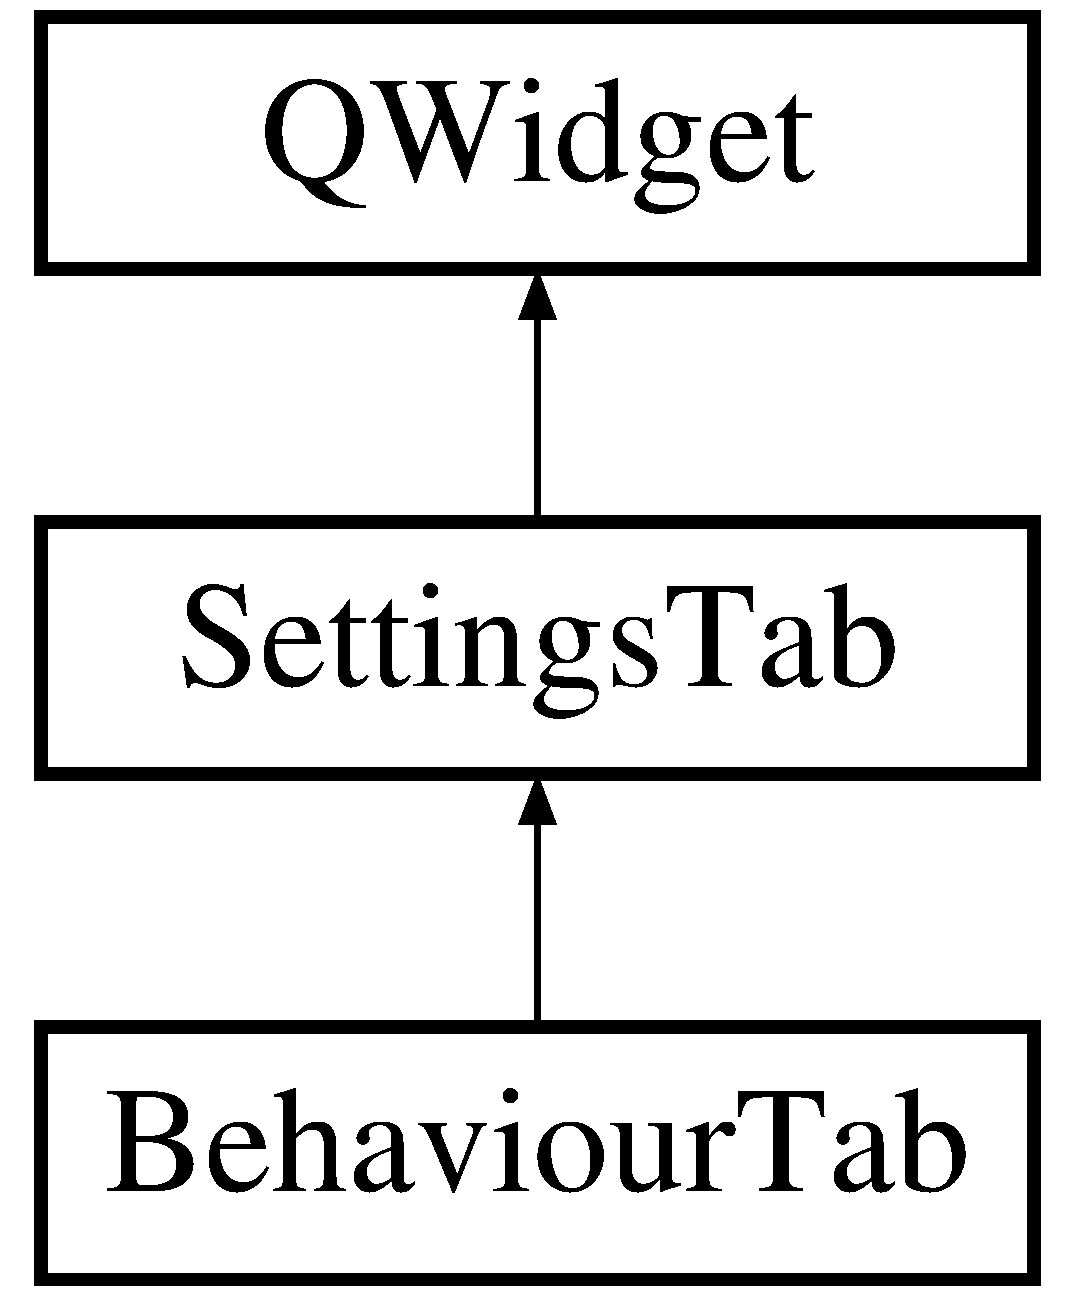
\includegraphics[height=3.000000cm]{classBehaviourTab}
\end{center}
\end{figure}
\subsection*{Signals}
\begin{DoxyCompactItemize}
\item 
\hypertarget{classSettingsTab_ab72744b5433a111f3e79da0ef1d9af74}{void {\bfseries content\+Changed} ()}\label{classSettingsTab_ab72744b5433a111f3e79da0ef1d9af74}

\end{DoxyCompactItemize}
\subsection*{Public Member Functions}
\begin{DoxyCompactItemize}
\item 
\hyperlink{classBehaviourTab_aef517fdf230f2ec647a314f61c435c16}{Behaviour\+Tab} (Q\+Hash$<$ Q\+String, Q\+Variant $>$ $\ast$Settings, Q\+Widget $\ast$parent=0)
\begin{DoxyCompactList}\small\item\em \hyperlink{classBehaviourTab_aef517fdf230f2ec647a314f61c435c16}{Behaviour\+Tab\+::\+Behaviour\+Tab}. \end{DoxyCompactList}\item 
\hyperlink{classBehaviourTab_abe229e738294990a30a9c0b3fde8d482}{$\sim$\+Behaviour\+Tab} ()
\begin{DoxyCompactList}\small\item\em \hyperlink{classBehaviourTab_abe229e738294990a30a9c0b3fde8d482}{Behaviour\+Tab\+::$\sim$\+Behaviour\+Tab}. \end{DoxyCompactList}\end{DoxyCompactItemize}
\subsection*{Protected Attributes}
\begin{DoxyCompactItemize}
\item 
\hypertarget{classSettingsTab_af6d39f524ae1d31aa8655c1957939287}{Q\+Hash$<$ Q\+String, Q\+Variant $>$ $\ast$ {\bfseries settings}}\label{classSettingsTab_af6d39f524ae1d31aa8655c1957939287}

\end{DoxyCompactItemize}


\subsection{Detailed Description}
The \hyperlink{classLayoutTab}{Layout\+Tab} class. 

\begin{DoxyAuthor}{Author}
Veit Heller(s0539501) \& Tobias Brosge(s0539713)
\end{DoxyAuthor}
A subclass of \hyperlink{classSettingsTab}{Settings\+Tab} that implements one of the tabs of the \hyperlink{classSettingsWindow}{Settings\+Window} in which all configurations regarding behaviour can be found. 

\subsection{Constructor \& Destructor Documentation}
\hypertarget{classBehaviourTab_aef517fdf230f2ec647a314f61c435c16}{\index{Behaviour\+Tab@{Behaviour\+Tab}!Behaviour\+Tab@{Behaviour\+Tab}}
\index{Behaviour\+Tab@{Behaviour\+Tab}!Behaviour\+Tab@{Behaviour\+Tab}}
\subsubsection[{Behaviour\+Tab}]{\setlength{\rightskip}{0pt plus 5cm}Behaviour\+Tab\+::\+Behaviour\+Tab (
\begin{DoxyParamCaption}
\item[{Q\+Hash$<$ Q\+String, Q\+Variant $>$ $\ast$}]{Settings, }
\item[{Q\+Widget $\ast$}]{parent = {\ttfamily 0}}
\end{DoxyParamCaption}
)}}\label{classBehaviourTab_aef517fdf230f2ec647a314f61c435c16}


\hyperlink{classBehaviourTab_aef517fdf230f2ec647a314f61c435c16}{Behaviour\+Tab\+::\+Behaviour\+Tab}. 

Construcotr of the \hyperlink{classBehaviourTab}{Behaviour\+Tab} class. Calls add\+Layout(). \hypertarget{classBehaviourTab_abe229e738294990a30a9c0b3fde8d482}{\index{Behaviour\+Tab@{Behaviour\+Tab}!````~Behaviour\+Tab@{$\sim$\+Behaviour\+Tab}}
\index{````~Behaviour\+Tab@{$\sim$\+Behaviour\+Tab}!Behaviour\+Tab@{Behaviour\+Tab}}
\subsubsection[{$\sim$\+Behaviour\+Tab}]{\setlength{\rightskip}{0pt plus 5cm}Behaviour\+Tab\+::$\sim$\+Behaviour\+Tab (
\begin{DoxyParamCaption}
{}
\end{DoxyParamCaption}
)}}\label{classBehaviourTab_abe229e738294990a30a9c0b3fde8d482}


\hyperlink{classBehaviourTab_abe229e738294990a30a9c0b3fde8d482}{Behaviour\+Tab\+::$\sim$\+Behaviour\+Tab}. 

Destructor of the \hyperlink{classBehaviourTab}{Behaviour\+Tab} class. Deletes the G\+U\+I elements. 

The documentation for this class was generated from the following files\+:\begin{DoxyCompactItemize}
\item 
src/Settings\+Tab.\+hpp\item 
src/Settings\+Tab.\+cpp\end{DoxyCompactItemize}

\hypertarget{classBootLoader}{\section{Boot\+Loader Class Reference}
\label{classBootLoader}\index{Boot\+Loader@{Boot\+Loader}}
}


The \hyperlink{classBootLoader}{Boot\+Loader} class.  




{\ttfamily \#include $<$Boot\+Loader.\+hpp$>$}

Inheritance diagram for Boot\+Loader\+:\begin{figure}[H]
\begin{center}
\leavevmode
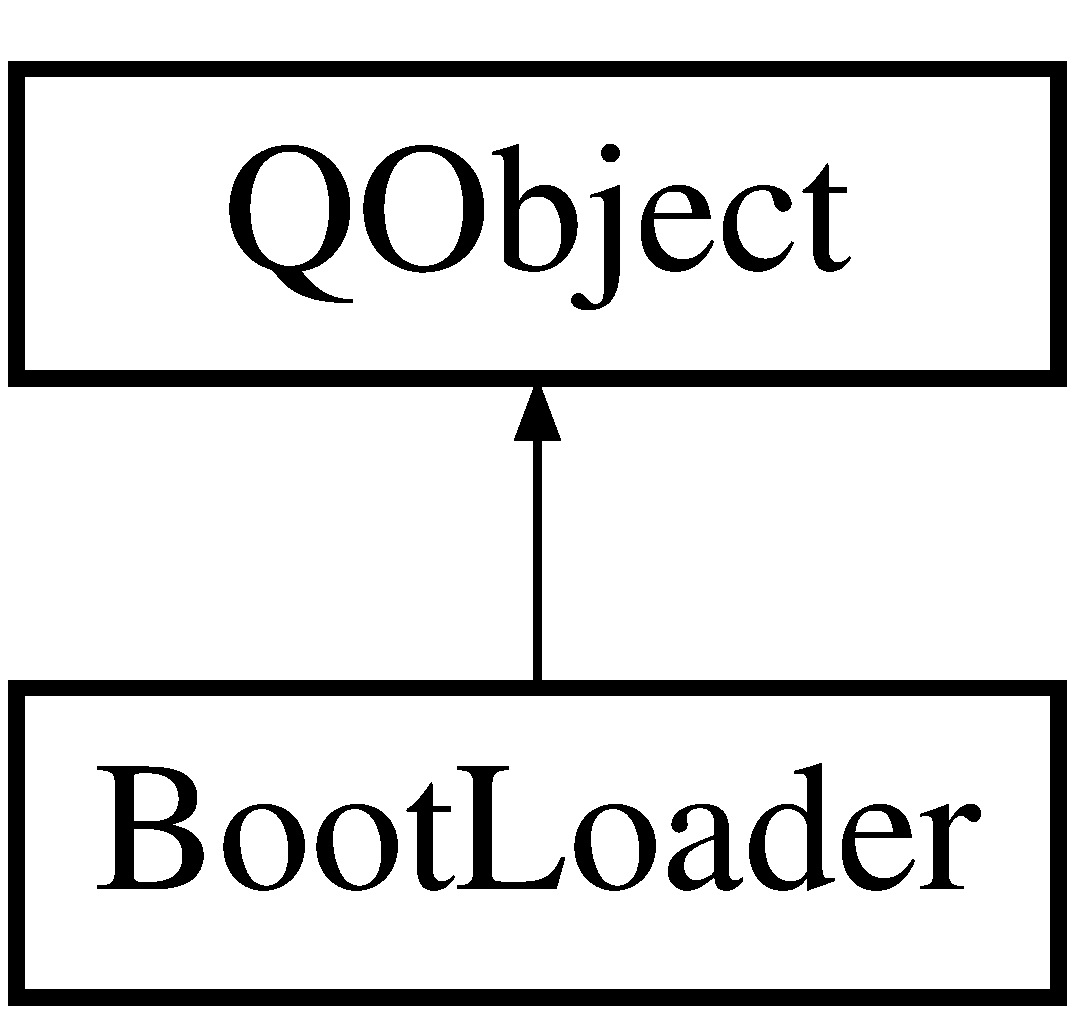
\includegraphics[height=2.000000cm]{classBootLoader}
\end{center}
\end{figure}
\subsection*{Public Slots}
\begin{DoxyCompactItemize}
\item 
void \hyperlink{classBootLoader_a2c367b2058dd21fd7d691fb6ba9fa4af}{accept\+Connection} ()
\begin{DoxyCompactList}\small\item\em \hyperlink{classBootLoader_a2c367b2058dd21fd7d691fb6ba9fa4af}{Boot\+Loader\+::accept\+Connection}. \end{DoxyCompactList}\end{DoxyCompactItemize}
\subsection*{Public Member Functions}
\begin{DoxyCompactItemize}
\item 
\hyperlink{classBootLoader_a086c590fb85e5311fbf3462f59e57bde}{Boot\+Loader} (const Q\+String \&socket\+Name, \hyperlink{classBackend}{Backend} $\ast$parent=0)
\begin{DoxyCompactList}\small\item\em \hyperlink{classBootLoader_a086c590fb85e5311fbf3462f59e57bde}{Boot\+Loader\+::\+Boot\+Loader}. \end{DoxyCompactList}\item 
\hyperlink{classBootLoader_ac290bb9c534fde124cde7c3081ccfb89}{$\sim$\+Boot\+Loader} ()
\begin{DoxyCompactList}\small\item\em \hyperlink{classBootLoader_ac290bb9c534fde124cde7c3081ccfb89}{Boot\+Loader\+::$\sim$\+Boot\+Loader}. \end{DoxyCompactList}\item 
void \hyperlink{classBootLoader_ada1e862287e0cdc87da083f475fbf68b}{start} ()
\begin{DoxyCompactList}\small\item\em \hyperlink{classBootLoader_ada1e862287e0cdc87da083f475fbf68b}{Boot\+Loader\+::start}. \end{DoxyCompactList}\end{DoxyCompactItemize}


\subsection{Detailed Description}
The \hyperlink{classBootLoader}{Boot\+Loader} class. 

A basic server that listens to new instances of the program being started and registering them with the main application. 

\subsection{Constructor \& Destructor Documentation}
\hypertarget{classBootLoader_a086c590fb85e5311fbf3462f59e57bde}{\index{Boot\+Loader@{Boot\+Loader}!Boot\+Loader@{Boot\+Loader}}
\index{Boot\+Loader@{Boot\+Loader}!Boot\+Loader@{Boot\+Loader}}
\subsubsection[{Boot\+Loader}]{\setlength{\rightskip}{0pt plus 5cm}Boot\+Loader\+::\+Boot\+Loader (
\begin{DoxyParamCaption}
\item[{const Q\+String \&}]{socket\+Name, }
\item[{{\bf Backend} $\ast$}]{parent = {\ttfamily 0}}
\end{DoxyParamCaption}
)\hspace{0.3cm}{\ttfamily [explicit]}}}\label{classBootLoader_a086c590fb85e5311fbf3462f59e57bde}


\hyperlink{classBootLoader_a086c590fb85e5311fbf3462f59e57bde}{Boot\+Loader\+::\+Boot\+Loader}. 


\begin{DoxyParams}{Parameters}
{\em socket\+Name} & \\
\hline
{\em parent} & Constructor of the \hyperlink{classBootLoader}{Boot\+Loader} class. instantiates the socket and registers with the parent. \\
\hline
\end{DoxyParams}
\hypertarget{classBootLoader_ac290bb9c534fde124cde7c3081ccfb89}{\index{Boot\+Loader@{Boot\+Loader}!````~Boot\+Loader@{$\sim$\+Boot\+Loader}}
\index{````~Boot\+Loader@{$\sim$\+Boot\+Loader}!Boot\+Loader@{Boot\+Loader}}
\subsubsection[{$\sim$\+Boot\+Loader}]{\setlength{\rightskip}{0pt plus 5cm}Boot\+Loader\+::$\sim$\+Boot\+Loader (
\begin{DoxyParamCaption}
{}
\end{DoxyParamCaption}
)}}\label{classBootLoader_ac290bb9c534fde124cde7c3081ccfb89}


\hyperlink{classBootLoader_ac290bb9c534fde124cde7c3081ccfb89}{Boot\+Loader\+::$\sim$\+Boot\+Loader}. 

Destructor of the Bootloader class. Cleans up the server. 

\subsection{Member Function Documentation}
\hypertarget{classBootLoader_a2c367b2058dd21fd7d691fb6ba9fa4af}{\index{Boot\+Loader@{Boot\+Loader}!accept\+Connection@{accept\+Connection}}
\index{accept\+Connection@{accept\+Connection}!Boot\+Loader@{Boot\+Loader}}
\subsubsection[{accept\+Connection}]{\setlength{\rightskip}{0pt plus 5cm}void Boot\+Loader\+::accept\+Connection (
\begin{DoxyParamCaption}
{}
\end{DoxyParamCaption}
)\hspace{0.3cm}{\ttfamily [slot]}}}\label{classBootLoader_a2c367b2058dd21fd7d691fb6ba9fa4af}


\hyperlink{classBootLoader_a2c367b2058dd21fd7d691fb6ba9fa4af}{Boot\+Loader\+::accept\+Connection}. 

Accepts a connection from a client, registers it with the backend(so it will run in the main app) and kills the original client. 

References Backend\+::add\+Instance(), and Backend\+::next\+I\+D().



Referenced by start().

\hypertarget{classBootLoader_ada1e862287e0cdc87da083f475fbf68b}{\index{Boot\+Loader@{Boot\+Loader}!start@{start}}
\index{start@{start}!Boot\+Loader@{Boot\+Loader}}
\subsubsection[{start}]{\setlength{\rightskip}{0pt plus 5cm}void Boot\+Loader\+::start (
\begin{DoxyParamCaption}
{}
\end{DoxyParamCaption}
)}}\label{classBootLoader_ada1e862287e0cdc87da083f475fbf68b}


\hyperlink{classBootLoader_ada1e862287e0cdc87da083f475fbf68b}{Boot\+Loader\+::start}. 

starts the Boot\+Loader/socket. runs asynchronously. 

References accept\+Connection().



The documentation for this class was generated from the following files\+:\begin{DoxyCompactItemize}
\item 
src/Boot\+Loader.\+hpp\item 
src/Boot\+Loader.\+cpp\end{DoxyCompactItemize}

\hypertarget{classCodeEditor}{\section{Code\+Editor Class Reference}
\label{classCodeEditor}\index{Code\+Editor@{Code\+Editor}}
}


The \hyperlink{classCodeEditor}{Code\+Editor} class.  




{\ttfamily \#include $<$Code\+Editor.\+hpp$>$}

Inheritance diagram for Code\+Editor\+:\begin{figure}[H]
\begin{center}
\leavevmode
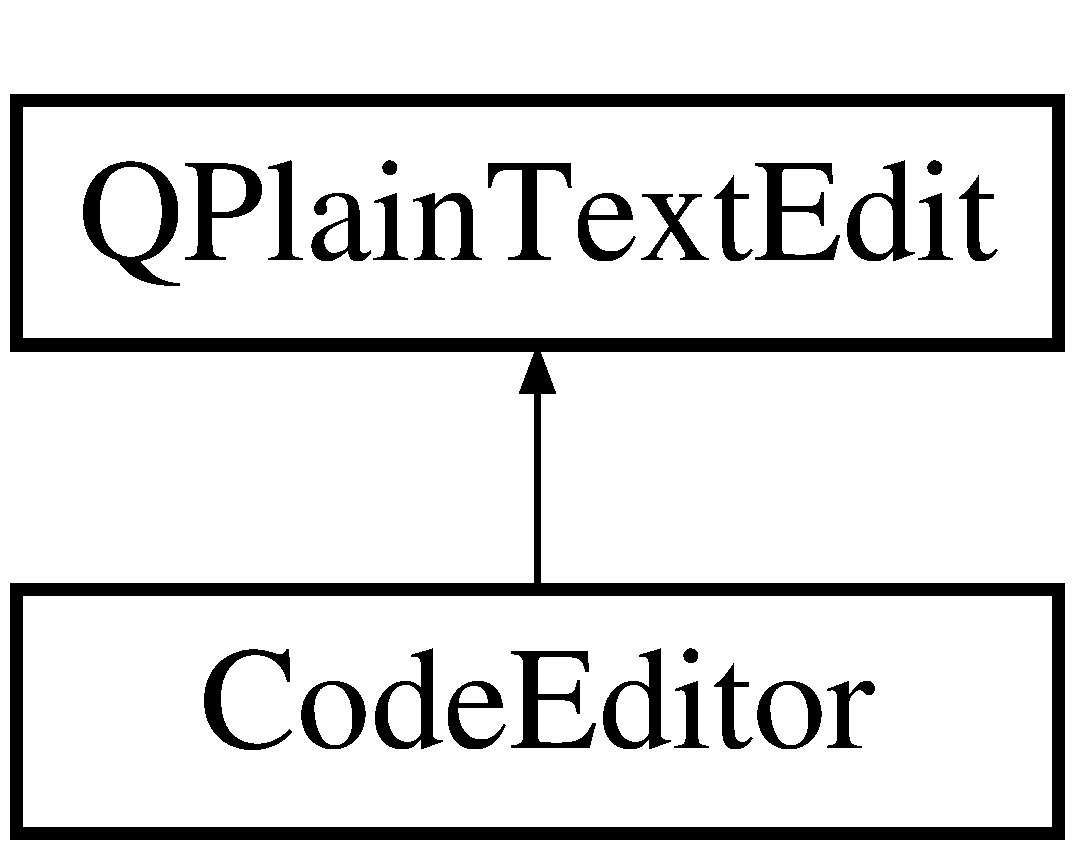
\includegraphics[height=2.000000cm]{classCodeEditor}
\end{center}
\end{figure}
\subsection*{Public Member Functions}
\begin{DoxyCompactItemize}
\item 
\hyperlink{classCodeEditor_a77c9d3d8aad039e7d0b0166737baac51}{Code\+Editor} (Q\+Widget $\ast$parent=0, int file=0)
\begin{DoxyCompactList}\small\item\em \hyperlink{classCodeEditor_a77c9d3d8aad039e7d0b0166737baac51}{Code\+Editor\+::\+Code\+Editor}. \end{DoxyCompactList}\item 
void \hyperlink{classCodeEditor_aaf6208c8c957341c1834cbe38c61d989}{line\+Highlighting\+Paint\+Event} (Q\+Paint\+Event $\ast$event)
\begin{DoxyCompactList}\small\item\em \hyperlink{classCodeEditor_aaf6208c8c957341c1834cbe38c61d989}{Code\+Editor\+::line\+Highlighting\+Paint\+Event}. \end{DoxyCompactList}\item 
int \hyperlink{classCodeEditor_afdce3b62e44a12089cb94a726916e53d}{line\+Highlighting\+Width} ()
\begin{DoxyCompactList}\small\item\em \hyperlink{classCodeEditor_afdce3b62e44a12089cb94a726916e53d}{Code\+Editor\+::line\+Highlighting\+Width}. \end{DoxyCompactList}\item 
void \hyperlink{classCodeEditor_aa2b0ad14f9e7a6a1aecd6b5b4d6b1480}{highlight\+Errored\+Line} (int)
\begin{DoxyCompactList}\small\item\em \hyperlink{classCodeEditor_aa2b0ad14f9e7a6a1aecd6b5b4d6b1480}{Code\+Editor\+::highlight\+Errored\+Line}. \end{DoxyCompactList}\item 
void \hyperlink{classCodeEditor_a3a8b18e7a1b4e00965d64c2816a770a8}{set\+Highlighting} (int highlighting)
\begin{DoxyCompactList}\small\item\em \hyperlink{classCodeEditor_a3a8b18e7a1b4e00965d64c2816a770a8}{Code\+Editor\+::set\+Highlighting}. \end{DoxyCompactList}\end{DoxyCompactItemize}
\subsection*{Protected Member Functions}
\begin{DoxyCompactItemize}
\item 
void \hyperlink{classCodeEditor_a3cf6c205d0cbcb3079811a406aab19be}{resize\+Event} (Q\+Resize\+Event $\ast$event)
\begin{DoxyCompactList}\small\item\em \hyperlink{classCodeEditor_a3cf6c205d0cbcb3079811a406aab19be}{Code\+Editor\+::resize\+Event}. \end{DoxyCompactList}\item 
void \hyperlink{classCodeEditor_aa7addc3f760c1503bf8a2e57bb4b8678}{key\+Press\+Event} (Q\+Key\+Event $\ast$e)
\begin{DoxyCompactList}\small\item\em \hyperlink{classCodeEditor_aa7addc3f760c1503bf8a2e57bb4b8678}{Code\+Editor\+::key\+Press\+Event}. \end{DoxyCompactList}\end{DoxyCompactItemize}


\subsection{Detailed Description}
The \hyperlink{classCodeEditor}{Code\+Editor} class. 

\begin{DoxyAuthor}{Author}
Veit Heller(s0539501) \& Tobias Brosge(s0539713)
\end{DoxyAuthor}
A subclass of Q\+Plain\+Text\+Edit that is optimized for code; with Syntax Highlighting, line numbers and highlighting of the current line. 

\subsection{Constructor \& Destructor Documentation}
\hypertarget{classCodeEditor_a77c9d3d8aad039e7d0b0166737baac51}{\index{Code\+Editor@{Code\+Editor}!Code\+Editor@{Code\+Editor}}
\index{Code\+Editor@{Code\+Editor}!Code\+Editor@{Code\+Editor}}
\subsubsection[{Code\+Editor}]{\setlength{\rightskip}{0pt plus 5cm}Code\+Editor\+::\+Code\+Editor (
\begin{DoxyParamCaption}
\item[{Q\+Widget $\ast$}]{parent = {\ttfamily 0}, }
\item[{int}]{file = {\ttfamily 0}}
\end{DoxyParamCaption}
)}}\label{classCodeEditor_a77c9d3d8aad039e7d0b0166737baac51}


\hyperlink{classCodeEditor_a77c9d3d8aad039e7d0b0166737baac51}{Code\+Editor\+::\+Code\+Editor}. 


\begin{DoxyParams}{Parameters}
{\em parent} & \\
\hline
{\em file} & The constructor of the code editor. Sets up the highlighting of syntax and current line and connects slots and signals. Needs a highlighting file. \\
\hline
\end{DoxyParams}


\subsection{Member Function Documentation}
\hypertarget{classCodeEditor_aa2b0ad14f9e7a6a1aecd6b5b4d6b1480}{\index{Code\+Editor@{Code\+Editor}!highlight\+Errored\+Line@{highlight\+Errored\+Line}}
\index{highlight\+Errored\+Line@{highlight\+Errored\+Line}!Code\+Editor@{Code\+Editor}}
\subsubsection[{highlight\+Errored\+Line}]{\setlength{\rightskip}{0pt plus 5cm}void Code\+Editor\+::highlight\+Errored\+Line (
\begin{DoxyParamCaption}
\item[{int}]{lineno}
\end{DoxyParamCaption}
)}}\label{classCodeEditor_aa2b0ad14f9e7a6a1aecd6b5b4d6b1480}


\hyperlink{classCodeEditor_aa2b0ad14f9e7a6a1aecd6b5b4d6b1480}{Code\+Editor\+::highlight\+Errored\+Line}. 


\begin{DoxyParams}{Parameters}
{\em lineno} & highlights the line given as argument as errored. \\
\hline
\end{DoxyParams}


Referenced by Editor\+Window\+::highlight\+Errored\+Line().

\hypertarget{classCodeEditor_aa7addc3f760c1503bf8a2e57bb4b8678}{\index{Code\+Editor@{Code\+Editor}!key\+Press\+Event@{key\+Press\+Event}}
\index{key\+Press\+Event@{key\+Press\+Event}!Code\+Editor@{Code\+Editor}}
\subsubsection[{key\+Press\+Event}]{\setlength{\rightskip}{0pt plus 5cm}void Code\+Editor\+::key\+Press\+Event (
\begin{DoxyParamCaption}
\item[{Q\+Key\+Event $\ast$}]{e}
\end{DoxyParamCaption}
)\hspace{0.3cm}{\ttfamily [protected]}}}\label{classCodeEditor_aa7addc3f760c1503bf8a2e57bb4b8678}


\hyperlink{classCodeEditor_aa7addc3f760c1503bf8a2e57bb4b8678}{Code\+Editor\+::key\+Press\+Event}. 


\begin{DoxyParams}{Parameters}
{\em e} & intercepts the key\+Press\+Event e so that a tab is rendered as 4 spaces. \\
\hline
\end{DoxyParams}
\hypertarget{classCodeEditor_aaf6208c8c957341c1834cbe38c61d989}{\index{Code\+Editor@{Code\+Editor}!line\+Highlighting\+Paint\+Event@{line\+Highlighting\+Paint\+Event}}
\index{line\+Highlighting\+Paint\+Event@{line\+Highlighting\+Paint\+Event}!Code\+Editor@{Code\+Editor}}
\subsubsection[{line\+Highlighting\+Paint\+Event}]{\setlength{\rightskip}{0pt plus 5cm}void Code\+Editor\+::line\+Highlighting\+Paint\+Event (
\begin{DoxyParamCaption}
\item[{Q\+Paint\+Event $\ast$}]{event}
\end{DoxyParamCaption}
)}}\label{classCodeEditor_aaf6208c8c957341c1834cbe38c61d989}


\hyperlink{classCodeEditor_aaf6208c8c957341c1834cbe38c61d989}{Code\+Editor\+::line\+Highlighting\+Paint\+Event}. 


\begin{DoxyParams}{Parameters}
{\em event} & updates the line highlighting whenever scrolling happens; invoked from update\+Line\+Highlighting(). \\
\hline
\end{DoxyParams}
\hypertarget{classCodeEditor_afdce3b62e44a12089cb94a726916e53d}{\index{Code\+Editor@{Code\+Editor}!line\+Highlighting\+Width@{line\+Highlighting\+Width}}
\index{line\+Highlighting\+Width@{line\+Highlighting\+Width}!Code\+Editor@{Code\+Editor}}
\subsubsection[{line\+Highlighting\+Width}]{\setlength{\rightskip}{0pt plus 5cm}int Code\+Editor\+::line\+Highlighting\+Width (
\begin{DoxyParamCaption}
{}
\end{DoxyParamCaption}
)}}\label{classCodeEditor_afdce3b62e44a12089cb94a726916e53d}


\hyperlink{classCodeEditor_afdce3b62e44a12089cb94a726916e53d}{Code\+Editor\+::line\+Highlighting\+Width}. 

\begin{DoxyReturn}{Returns}
the width of the line to be highlighted
\end{DoxyReturn}
Helper function that computes the width of the line that is to be highlighted. 

Referenced by resize\+Event().

\hypertarget{classCodeEditor_a3cf6c205d0cbcb3079811a406aab19be}{\index{Code\+Editor@{Code\+Editor}!resize\+Event@{resize\+Event}}
\index{resize\+Event@{resize\+Event}!Code\+Editor@{Code\+Editor}}
\subsubsection[{resize\+Event}]{\setlength{\rightskip}{0pt plus 5cm}void Code\+Editor\+::resize\+Event (
\begin{DoxyParamCaption}
\item[{Q\+Resize\+Event $\ast$}]{e}
\end{DoxyParamCaption}
)\hspace{0.3cm}{\ttfamily [protected]}}}\label{classCodeEditor_a3cf6c205d0cbcb3079811a406aab19be}


\hyperlink{classCodeEditor_a3cf6c205d0cbcb3079811a406aab19be}{Code\+Editor\+::resize\+Event}. 


\begin{DoxyParams}{Parameters}
{\em e} & catches the resize signal and customizes the update(\+S\+L\+O\+T) \\
\hline
\end{DoxyParams}


References line\+Highlighting\+Width().

\hypertarget{classCodeEditor_a3a8b18e7a1b4e00965d64c2816a770a8}{\index{Code\+Editor@{Code\+Editor}!set\+Highlighting@{set\+Highlighting}}
\index{set\+Highlighting@{set\+Highlighting}!Code\+Editor@{Code\+Editor}}
\subsubsection[{set\+Highlighting}]{\setlength{\rightskip}{0pt plus 5cm}void Code\+Editor\+::set\+Highlighting (
\begin{DoxyParamCaption}
\item[{int}]{highlighting}
\end{DoxyParamCaption}
)}}\label{classCodeEditor_a3a8b18e7a1b4e00965d64c2816a770a8}


\hyperlink{classCodeEditor_a3a8b18e7a1b4e00965d64c2816a770a8}{Code\+Editor\+::set\+Highlighting}. 


\begin{DoxyParams}{Parameters}
{\em highlighting} & Tells the syntax highlighter to change highlighting by using a code where 0 and 3 stand for Python, 1 stands for Qt and 2 stands for G\+L\+S\+L. \\
\hline
\end{DoxyParams}


References Code\+Highlighter\+::setup\+Highlighting().



The documentation for this class was generated from the following files\+:\begin{DoxyCompactItemize}
\item 
src/Code\+Editor.\+hpp\item 
src/Code\+Editor.\+cpp\end{DoxyCompactItemize}

\hypertarget{classCodeHighlighter}{\section{Code\+Highlighter Class Reference}
\label{classCodeHighlighter}\index{Code\+Highlighter@{Code\+Highlighter}}
}


The \hyperlink{classCodeHighlighter}{Code\+Highlighter} class.  




{\ttfamily \#include $<$Code\+Highlighter.\+hpp$>$}

Inheritance diagram for Code\+Highlighter\+:\begin{figure}[H]
\begin{center}
\leavevmode
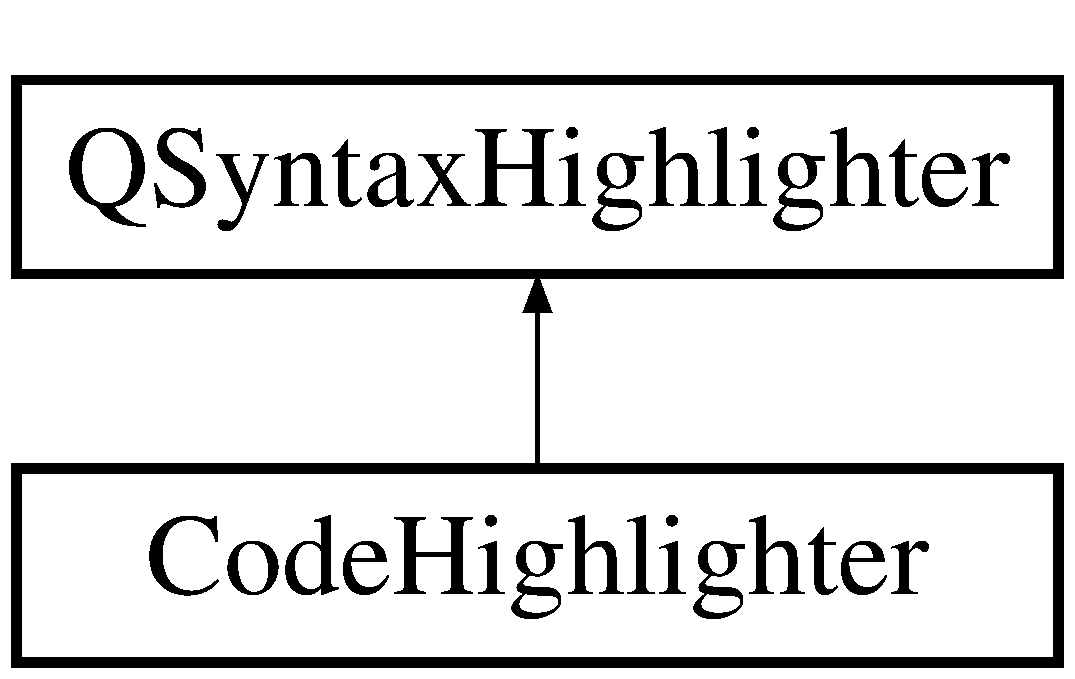
\includegraphics[height=2.000000cm]{classCodeHighlighter}
\end{center}
\end{figure}
\subsection*{Public Member Functions}
\begin{DoxyCompactItemize}
\item 
\hyperlink{classCodeHighlighter_aefbf2c4ec8b87c39aac8b4caf516765b}{Code\+Highlighter} (Q\+Text\+Document $\ast$parent=0, int file=0)
\begin{DoxyCompactList}\small\item\em \hyperlink{classCodeHighlighter_aefbf2c4ec8b87c39aac8b4caf516765b}{Code\+Highlighter\+::\+Code\+Highlighter}. \end{DoxyCompactList}\item 
bool \hyperlink{classCodeHighlighter_a61d21b1d88b955403a5d1e3601a22353}{setup\+Highlighting} (int file)
\begin{DoxyCompactList}\small\item\em \hyperlink{classCodeHighlighter_a61d21b1d88b955403a5d1e3601a22353}{Code\+Highlighter\+::setup\+Highlighting}. \end{DoxyCompactList}\item 
\hypertarget{classCodeHighlighter_a77d779445aeca5953113634e982ffac8}{int {\bfseries get\+Highlighting} ()}\label{classCodeHighlighter_a77d779445aeca5953113634e982ffac8}

\end{DoxyCompactItemize}
\subsection*{Protected Member Functions}
\begin{DoxyCompactItemize}
\item 
void \hyperlink{classCodeHighlighter_a38e1190233f89b655e84aaef864b2e76}{highlight\+Block} (const Q\+String \&text)
\begin{DoxyCompactList}\small\item\em \hyperlink{classCodeHighlighter_a38e1190233f89b655e84aaef864b2e76}{Code\+Highlighter\+::highlight\+Block}. \end{DoxyCompactList}\end{DoxyCompactItemize}


\subsection{Detailed Description}
The \hyperlink{classCodeHighlighter}{Code\+Highlighter} class. 

\begin{DoxyAuthor}{Author}
Veit Heller(s0539501) \& Tobias Brosge(s0539713)
\end{DoxyAuthor}
A subclass of Q\+Syntax\+Highlighter that implements Syntax Highlighting(duh!) for the Code Editor class. 

\subsection{Constructor \& Destructor Documentation}
\hypertarget{classCodeHighlighter_aefbf2c4ec8b87c39aac8b4caf516765b}{\index{Code\+Highlighter@{Code\+Highlighter}!Code\+Highlighter@{Code\+Highlighter}}
\index{Code\+Highlighter@{Code\+Highlighter}!Code\+Highlighter@{Code\+Highlighter}}
\subsubsection[{Code\+Highlighter}]{\setlength{\rightskip}{0pt plus 5cm}Code\+Highlighter\+::\+Code\+Highlighter (
\begin{DoxyParamCaption}
\item[{Q\+Text\+Document $\ast$}]{parent = {\ttfamily 0}, }
\item[{int}]{file = {\ttfamily 0}}
\end{DoxyParamCaption}
)}}\label{classCodeHighlighter_aefbf2c4ec8b87c39aac8b4caf516765b}


\hyperlink{classCodeHighlighter_aefbf2c4ec8b87c39aac8b4caf516765b}{Code\+Highlighter\+::\+Code\+Highlighter}. 


\begin{DoxyParams}{Parameters}
{\em parent} & \\
\hline
{\em file} & The constructor of the syntax highlighter. Needs a highlighting file. \\
\hline
\end{DoxyParams}


References setup\+Highlighting().



\subsection{Member Function Documentation}
\hypertarget{classCodeHighlighter_a38e1190233f89b655e84aaef864b2e76}{\index{Code\+Highlighter@{Code\+Highlighter}!highlight\+Block@{highlight\+Block}}
\index{highlight\+Block@{highlight\+Block}!Code\+Highlighter@{Code\+Highlighter}}
\subsubsection[{highlight\+Block}]{\setlength{\rightskip}{0pt plus 5cm}void Code\+Highlighter\+::highlight\+Block (
\begin{DoxyParamCaption}
\item[{const Q\+String \&}]{text}
\end{DoxyParamCaption}
)\hspace{0.3cm}{\ttfamily [protected]}}}\label{classCodeHighlighter_a38e1190233f89b655e84aaef864b2e76}


\hyperlink{classCodeHighlighter_a38e1190233f89b655e84aaef864b2e76}{Code\+Highlighter\+::highlight\+Block}. 


\begin{DoxyParams}{Parameters}
{\em text} & Highlights blocks(duh) by evaluating the regexes created in the constructor. T\+O\+D\+O\+: Code and time complexity are suboptimal. Is there a better way? \\
\hline
\end{DoxyParams}
\hypertarget{classCodeHighlighter_a61d21b1d88b955403a5d1e3601a22353}{\index{Code\+Highlighter@{Code\+Highlighter}!setup\+Highlighting@{setup\+Highlighting}}
\index{setup\+Highlighting@{setup\+Highlighting}!Code\+Highlighter@{Code\+Highlighter}}
\subsubsection[{setup\+Highlighting}]{\setlength{\rightskip}{0pt plus 5cm}bool Code\+Highlighter\+::setup\+Highlighting (
\begin{DoxyParamCaption}
\item[{int}]{file}
\end{DoxyParamCaption}
)}}\label{classCodeHighlighter_a61d21b1d88b955403a5d1e3601a22353}


\hyperlink{classCodeHighlighter_a61d21b1d88b955403a5d1e3601a22353}{Code\+Highlighter\+::setup\+Highlighting}. 


\begin{DoxyParams}{Parameters}
{\em file} & Sets up the highlighting rules. T\+O\+D\+O\+: Make it more flexible -\/ File format? T\+O\+D\+O\+: Highlight bracket-\/pairs T\+O\+D\+O\+: Build quot-\/pairs ( \char`\"{}bla \char`\"{} bla \char`\"{} bla \char`\"{} -\/$>$ all is highlighted) T\+O\+D\+O\+: don't let the multi line comment trust preview format (see function highlight\+Block(...) ) \\
\hline
\end{DoxyParams}


Referenced by Code\+Highlighter(), and Code\+Editor\+::set\+Highlighting().



The documentation for this class was generated from the following files\+:\begin{DoxyCompactItemize}
\item 
src/Code\+Highlighter.\+hpp\item 
src/Code\+Highlighter.\+cpp\end{DoxyCompactItemize}

\hypertarget{classEditorWindow}{\section{Editor\+Window Class Reference}
\label{classEditorWindow}\index{Editor\+Window@{Editor\+Window}}
}


The \hyperlink{classEditorWindow}{Editor\+Window} class.  




{\ttfamily \#include $<$Editor\+Window.\+hpp$>$}

Inheritance diagram for Editor\+Window\+:\begin{figure}[H]
\begin{center}
\leavevmode
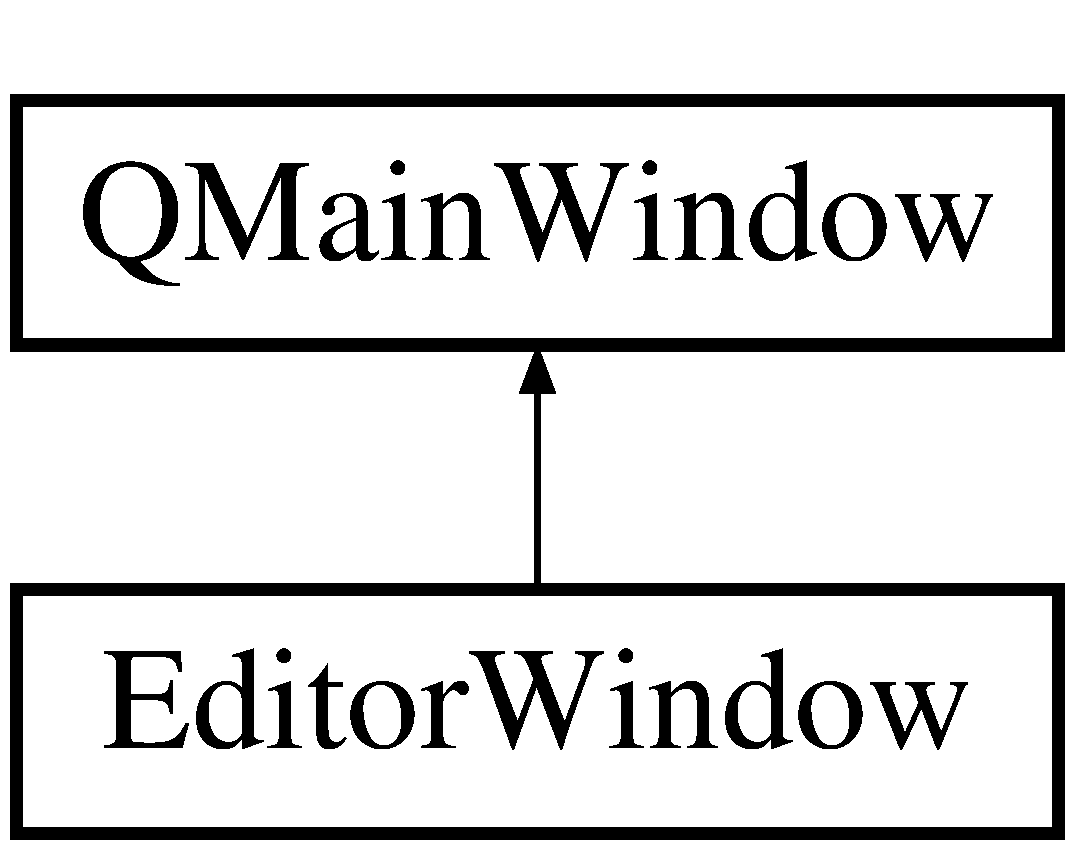
\includegraphics[height=2.000000cm]{classEditorWindow}
\end{center}
\end{figure}
\subsection*{Signals}
\begin{DoxyCompactItemize}
\item 
\hypertarget{classEditorWindow_ab5059ac20da670e1c2bb3e7e6e498aa1}{void {\bfseries closing} (\hyperlink{classEditorWindow}{Editor\+Window} $\ast$)}\label{classEditorWindow_ab5059ac20da670e1c2bb3e7e6e498aa1}

\item 
\hypertarget{classEditorWindow_a8e82f25b8aaa98fdcbd80ffbf4f2f01c}{void {\bfseries close\+All} (\hyperlink{classEditorWindow}{Editor\+Window} $\ast$)}\label{classEditorWindow_a8e82f25b8aaa98fdcbd80ffbf4f2f01c}

\item 
\hypertarget{classEditorWindow_a5a18c4334a66f2152f814690f27423c7}{void {\bfseries open\+Settings} (\hyperlink{classEditorWindow}{Editor\+Window} $\ast$)}\label{classEditorWindow_a5a18c4334a66f2152f814690f27423c7}

\item 
\hypertarget{classEditorWindow_a12b01e035aef46c087d4fa972748b4c9}{void {\bfseries open\+Help} (\hyperlink{classEditorWindow}{Editor\+Window} $\ast$)}\label{classEditorWindow_a12b01e035aef46c087d4fa972748b4c9}

\item 
\hypertarget{classEditorWindow_a099b128c5e948867df18babd7c6b14ca}{void {\bfseries run\+Code} (\hyperlink{classEditorWindow}{Editor\+Window} $\ast$)}\label{classEditorWindow_a099b128c5e948867df18babd7c6b14ca}

\item 
\hypertarget{classEditorWindow_af4ca2e0be1bb3098a8c94473c753d9c2}{void {\bfseries stop\+Code} (\hyperlink{classEditorWindow}{Editor\+Window} $\ast$)}\label{classEditorWindow_af4ca2e0be1bb3098a8c94473c753d9c2}

\item 
\hypertarget{classEditorWindow_a3927cefb23e1026ca7362c99da5f144c}{void {\bfseries title\+Changed} (\hyperlink{classEditorWindow}{Editor\+Window} $\ast$)}\label{classEditorWindow_a3927cefb23e1026ca7362c99da5f144c}

\item 
\hypertarget{classEditorWindow_a512fc6a54509b75d26cdd3b13eae03eb}{void {\bfseries changed\+Setting} (\hyperlink{classEditorWindow}{Editor\+Window} $\ast$, const Q\+String \&, const Q\+Variant \&)}\label{classEditorWindow_a512fc6a54509b75d26cdd3b13eae03eb}

\item 
\hypertarget{classEditorWindow_a7ae350466d88e3d4aeadb5926217809a}{void {\bfseries changed\+Settings} (\hyperlink{classEditorWindow}{Editor\+Window} $\ast$, const Q\+Hash$<$ Q\+String, Q\+Variant $>$ \&)}\label{classEditorWindow_a7ae350466d88e3d4aeadb5926217809a}

\end{DoxyCompactItemize}
\subsection*{Public Member Functions}
\begin{DoxyCompactItemize}
\item 
\hyperlink{classEditorWindow_a6917407d81bd85ebc2af2f3915f62d56}{Editor\+Window} (const Q\+Hash$<$ Q\+String, Q\+Variant $>$ \&settings, Q\+Widget $\ast$parent=0)
\begin{DoxyCompactList}\small\item\em \hyperlink{classEditorWindow_a6917407d81bd85ebc2af2f3915f62d56}{Editor\+Window\+::\+Editor\+Window}. \end{DoxyCompactList}\item 
\hyperlink{classEditorWindow_a7dd5c84136960d8ba831b04993811cf3}{$\sim$\+Editor\+Window} ()
\begin{DoxyCompactList}\small\item\em \hyperlink{classEditorWindow_a7dd5c84136960d8ba831b04993811cf3}{Editor\+Window\+::$\sim$\+Editor\+Window}. \end{DoxyCompactList}\item 
void \hyperlink{classEditorWindow_a0ad1d080a548df7eb21ce05c50775e70}{show\+Results} (const Q\+String \&)
\begin{DoxyCompactList}\small\item\em \hyperlink{classEditorWindow_a0ad1d080a548df7eb21ce05c50775e70}{Editor\+Window\+::show\+Results}. \end{DoxyCompactList}\item 
void \hyperlink{classEditorWindow_ac40c7db381c4aa179667cc3803503880}{warning\+Display} (const Q\+String \&)
\begin{DoxyCompactList}\small\item\em \hyperlink{classEditorWindow_ac40c7db381c4aa179667cc3803503880}{Editor\+Window\+::warning\+Display}. \end{DoxyCompactList}\item 
void \hyperlink{classEditorWindow_af965f642e397d238c963df15e8561694}{highlight\+Errored\+Line} (int)
\begin{DoxyCompactList}\small\item\em \hyperlink{classEditorWindow_af965f642e397d238c963df15e8561694}{Editor\+Window\+::highlight\+Errored\+Line}. \end{DoxyCompactList}\item 
void \hyperlink{classEditorWindow_a03cc1e6ae0c550c6f5fff486eaf6b508}{code\+Stopped} ()
\begin{DoxyCompactList}\small\item\em \hyperlink{classEditorWindow_a03cc1e6ae0c550c6f5fff486eaf6b508}{Editor\+Window\+::code\+Stopped}. \end{DoxyCompactList}\item 
Q\+String \hyperlink{classEditorWindow_a4f42ffd31afc2a5e312f49048eab82ad}{get\+Source\+Code} () const 
\begin{DoxyCompactList}\small\item\em \hyperlink{classEditorWindow_a4f42ffd31afc2a5e312f49048eab82ad}{Editor\+Window\+::get\+Source\+Code}. \end{DoxyCompactList}\item 
Q\+String \hyperlink{classEditorWindow_a73910f42d7ffc26999f2d985fdc78686}{get\+Title} () const 
\begin{DoxyCompactList}\small\item\em \hyperlink{classEditorWindow_a73910f42d7ffc26999f2d985fdc78686}{Editor\+Window\+::get\+Title}. \end{DoxyCompactList}\end{DoxyCompactItemize}
\subsection*{Protected Member Functions}
\begin{DoxyCompactItemize}
\item 
virtual void \hyperlink{classEditorWindow_a70f0ac46ae9cd0362e1c4b80322c5fd6}{close\+Event} (Q\+Close\+Event $\ast$)
\begin{DoxyCompactList}\small\item\em \hyperlink{classEditorWindow_a70f0ac46ae9cd0362e1c4b80322c5fd6}{Editor\+Window\+::close\+Event}. \end{DoxyCompactList}\end{DoxyCompactItemize}


\subsection{Detailed Description}
The \hyperlink{classEditorWindow}{Editor\+Window} class. 

\begin{DoxyAuthor}{Author}
Veit Heller(s0539501) \& Tobias Brosge(s0539713)
\end{DoxyAuthor}
A subclass of Q\+Main\+Window that makes the \hyperlink{classCodeEditor}{Code\+Editor} more interactive by implementing save/load and open/close features. 

\subsection{Constructor \& Destructor Documentation}
\hypertarget{classEditorWindow_a6917407d81bd85ebc2af2f3915f62d56}{\index{Editor\+Window@{Editor\+Window}!Editor\+Window@{Editor\+Window}}
\index{Editor\+Window@{Editor\+Window}!Editor\+Window@{Editor\+Window}}
\subsubsection[{Editor\+Window}]{\setlength{\rightskip}{0pt plus 5cm}Editor\+Window\+::\+Editor\+Window (
\begin{DoxyParamCaption}
\item[{const Q\+Hash$<$ Q\+String, Q\+Variant $>$ \&}]{settings, }
\item[{Q\+Widget $\ast$}]{parent = {\ttfamily 0}}
\end{DoxyParamCaption}
)}}\label{classEditorWindow_a6917407d81bd85ebc2af2f3915f62d56}


\hyperlink{classEditorWindow_a6917407d81bd85ebc2af2f3915f62d56}{Editor\+Window\+::\+Editor\+Window}. 

The constructor of the \hyperlink{classEditorWindow}{Editor\+Window} class. Sets up the whole U\+I around the Editor, including slots and signals. Also loads the settings and loads the file that was last displayed when closing the editor. Also, it deals with platform-\/specific displaying quirks. \hypertarget{classEditorWindow_a7dd5c84136960d8ba831b04993811cf3}{\index{Editor\+Window@{Editor\+Window}!````~Editor\+Window@{$\sim$\+Editor\+Window}}
\index{````~Editor\+Window@{$\sim$\+Editor\+Window}!Editor\+Window@{Editor\+Window}}
\subsubsection[{$\sim$\+Editor\+Window}]{\setlength{\rightskip}{0pt plus 5cm}Editor\+Window\+::$\sim$\+Editor\+Window (
\begin{DoxyParamCaption}
{}
\end{DoxyParamCaption}
)}}\label{classEditorWindow_a7dd5c84136960d8ba831b04993811cf3}


\hyperlink{classEditorWindow_a7dd5c84136960d8ba831b04993811cf3}{Editor\+Window\+::$\sim$\+Editor\+Window}. 

Destructor of the \hyperlink{classEditorWindow}{Editor\+Window} class. Deletes all the G\+U\+I elements. 

\subsection{Member Function Documentation}
\hypertarget{classEditorWindow_a70f0ac46ae9cd0362e1c4b80322c5fd6}{\index{Editor\+Window@{Editor\+Window}!close\+Event@{close\+Event}}
\index{close\+Event@{close\+Event}!Editor\+Window@{Editor\+Window}}
\subsubsection[{close\+Event}]{\setlength{\rightskip}{0pt plus 5cm}void Editor\+Window\+::close\+Event (
\begin{DoxyParamCaption}
\item[{Q\+Close\+Event $\ast$}]{event}
\end{DoxyParamCaption}
)\hspace{0.3cm}{\ttfamily [protected]}, {\ttfamily [virtual]}}}\label{classEditorWindow_a70f0ac46ae9cd0362e1c4b80322c5fd6}


\hyperlink{classEditorWindow_a70f0ac46ae9cd0362e1c4b80322c5fd6}{Editor\+Window\+::close\+Event}. 


\begin{DoxyParams}{Parameters}
{\em event} & reacts to the close signal; saves the current preferences if wanted and exits(\+S\+L\+O\+T). \\
\hline
\end{DoxyParams}
\hypertarget{classEditorWindow_a03cc1e6ae0c550c6f5fff486eaf6b508}{\index{Editor\+Window@{Editor\+Window}!code\+Stopped@{code\+Stopped}}
\index{code\+Stopped@{code\+Stopped}!Editor\+Window@{Editor\+Window}}
\subsubsection[{code\+Stopped}]{\setlength{\rightskip}{0pt plus 5cm}void Editor\+Window\+::code\+Stopped (
\begin{DoxyParamCaption}
{}
\end{DoxyParamCaption}
)}}\label{classEditorWindow_a03cc1e6ae0c550c6f5fff486eaf6b508}


\hyperlink{classEditorWindow_a03cc1e6ae0c550c6f5fff486eaf6b508}{Editor\+Window\+::code\+Stopped}. 

Sets the icon back to normal. 

Referenced by Instances\+::\+Window\+Instance\+::code\+Stopped().

\hypertarget{classEditorWindow_a4f42ffd31afc2a5e312f49048eab82ad}{\index{Editor\+Window@{Editor\+Window}!get\+Source\+Code@{get\+Source\+Code}}
\index{get\+Source\+Code@{get\+Source\+Code}!Editor\+Window@{Editor\+Window}}
\subsubsection[{get\+Source\+Code}]{\setlength{\rightskip}{0pt plus 5cm}Q\+String Editor\+Window\+::get\+Source\+Code (
\begin{DoxyParamCaption}
{}
\end{DoxyParamCaption}
) const}}\label{classEditorWindow_a4f42ffd31afc2a5e312f49048eab82ad}


\hyperlink{classEditorWindow_a4f42ffd31afc2a5e312f49048eab82ad}{Editor\+Window\+::get\+Source\+Code}. 

\begin{DoxyReturn}{Returns}
plain text in editor
\end{DoxyReturn}
returns code in editor. 

Referenced by Instances\+::\+Window\+Instance\+::source\+Code().

\hypertarget{classEditorWindow_a73910f42d7ffc26999f2d985fdc78686}{\index{Editor\+Window@{Editor\+Window}!get\+Title@{get\+Title}}
\index{get\+Title@{get\+Title}!Editor\+Window@{Editor\+Window}}
\subsubsection[{get\+Title}]{\setlength{\rightskip}{0pt plus 5cm}Q\+String Editor\+Window\+::get\+Title (
\begin{DoxyParamCaption}
{}
\end{DoxyParamCaption}
) const}}\label{classEditorWindow_a73910f42d7ffc26999f2d985fdc78686}


\hyperlink{classEditorWindow_a73910f42d7ffc26999f2d985fdc78686}{Editor\+Window\+::get\+Title}. 

\begin{DoxyReturn}{Returns}
current file name as string.
\end{DoxyReturn}
returns current file name. 

Referenced by Instances\+::\+Window\+Instance\+::title().

\hypertarget{classEditorWindow_af965f642e397d238c963df15e8561694}{\index{Editor\+Window@{Editor\+Window}!highlight\+Errored\+Line@{highlight\+Errored\+Line}}
\index{highlight\+Errored\+Line@{highlight\+Errored\+Line}!Editor\+Window@{Editor\+Window}}
\subsubsection[{highlight\+Errored\+Line}]{\setlength{\rightskip}{0pt plus 5cm}void Editor\+Window\+::highlight\+Errored\+Line (
\begin{DoxyParamCaption}
\item[{int}]{lineno}
\end{DoxyParamCaption}
)}}\label{classEditorWindow_af965f642e397d238c963df15e8561694}


\hyperlink{classEditorWindow_af965f642e397d238c963df15e8561694}{Editor\+Window\+::highlight\+Errored\+Line}. 


\begin{DoxyParams}{Parameters}
{\em lineno} & Highlights a given line in red. Signifies an error in that line. \\
\hline
\end{DoxyParams}


References Code\+Editor\+::highlight\+Errored\+Line().



Referenced by Instances\+::\+Window\+Instance\+::highlight\+Errored\+Line().

\hypertarget{classEditorWindow_a0ad1d080a548df7eb21ce05c50775e70}{\index{Editor\+Window@{Editor\+Window}!show\+Results@{show\+Results}}
\index{show\+Results@{show\+Results}!Editor\+Window@{Editor\+Window}}
\subsubsection[{show\+Results}]{\setlength{\rightskip}{0pt plus 5cm}void Editor\+Window\+::show\+Results (
\begin{DoxyParamCaption}
\item[{const Q\+String \&}]{returned\+Value}
\end{DoxyParamCaption}
)}}\label{classEditorWindow_a0ad1d080a548df7eb21ce05c50775e70}


\hyperlink{classEditorWindow_a0ad1d080a548df7eb21ce05c50775e70}{Editor\+Window\+::show\+Results}. 


\begin{DoxyParams}{Parameters}
{\em returned\+Value} & Is called after the execution of the interpreter thread has finished. Shows its return code or an exception traceback. \\
\hline
\end{DoxyParams}


Referenced by Instances\+::\+Window\+Instance\+::report\+Warning().

\hypertarget{classEditorWindow_ac40c7db381c4aa179667cc3803503880}{\index{Editor\+Window@{Editor\+Window}!warning\+Display@{warning\+Display}}
\index{warning\+Display@{warning\+Display}!Editor\+Window@{Editor\+Window}}
\subsubsection[{warning\+Display}]{\setlength{\rightskip}{0pt plus 5cm}void Editor\+Window\+::warning\+Display (
\begin{DoxyParamCaption}
\item[{const Q\+String \&}]{message}
\end{DoxyParamCaption}
)}}\label{classEditorWindow_ac40c7db381c4aa179667cc3803503880}


\hyperlink{classEditorWindow_ac40c7db381c4aa179667cc3803503880}{Editor\+Window\+::warning\+Display}. 


\begin{DoxyParams}{Parameters}
{\em message} & Displays a warning box containing message. \\
\hline
\end{DoxyParams}


Referenced by Instances\+::\+Window\+Instance\+::report\+Error().



The documentation for this class was generated from the following files\+:\begin{DoxyCompactItemize}
\item 
src/Editor\+Window.\+hpp\item 
src/Editor\+Window.\+cpp\end{DoxyCompactItemize}

\hypertarget{classGlLiveThread}{\section{Gl\+Live\+Thread Class Reference}
\label{classGlLiveThread}\index{Gl\+Live\+Thread@{Gl\+Live\+Thread}}
}
Inheritance diagram for Gl\+Live\+Thread\+:\begin{figure}[H]
\begin{center}
\leavevmode
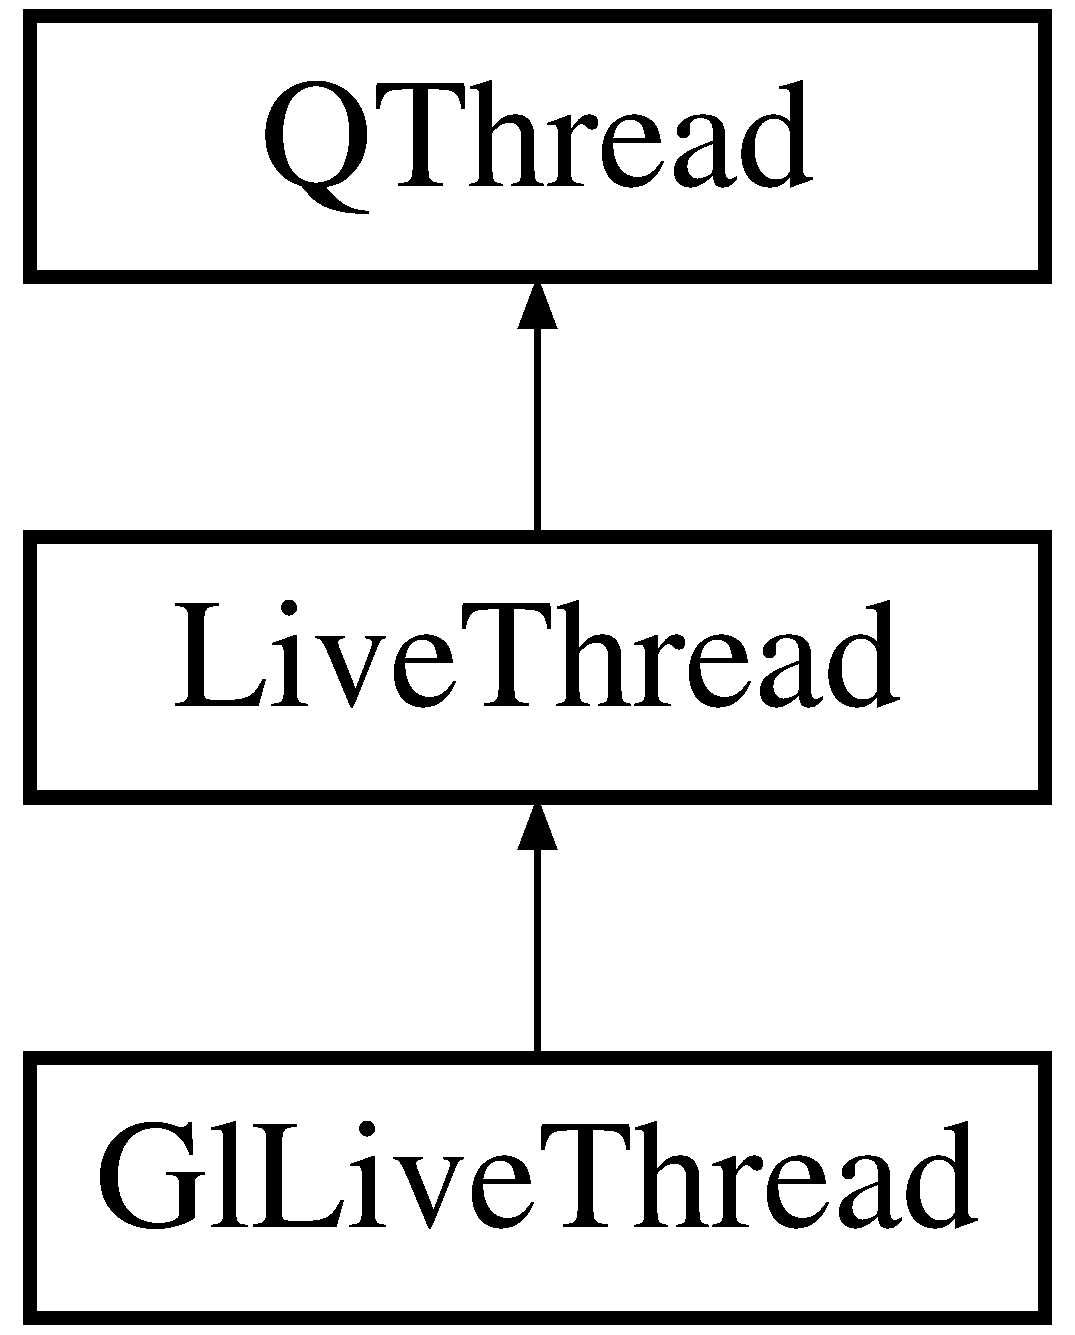
\includegraphics[height=3.000000cm]{classGlLiveThread}
\end{center}
\end{figure}
\subsection*{Public Slots}
\begin{DoxyCompactItemize}
\item 
\hypertarget{classGlLiveThread_af6fd5e5395e5a08d44b7d666209c36a3}{void {\bfseries done\+Signal\+Received} (Q\+String exception)}\label{classGlLiveThread_af6fd5e5395e5a08d44b7d666209c36a3}

\item 
\hypertarget{classGlLiveThread_a070e3978c7bcf1121e6343f6dcf54847}{void {\bfseries errored\+Received} (Q\+String error, int lineno)}\label{classGlLiveThread_a070e3978c7bcf1121e6343f6dcf54847}

\end{DoxyCompactItemize}
\subsection*{Signals}
\begin{DoxyCompactItemize}
\item 
\hypertarget{classGlLiveThread_aaf79277230ec2aae08bad4db48c2614c}{void {\bfseries done\+Signal} (\hyperlink{classGlLiveThread}{Gl\+Live\+Thread} $\ast$, Q\+String)}\label{classGlLiveThread_aaf79277230ec2aae08bad4db48c2614c}

\item 
\hypertarget{classGlLiveThread_ad8563a7fcd4dc42d1dcf7a85b087d40e}{void {\bfseries error\+Signal} (\hyperlink{classGlLiveThread}{Gl\+Live\+Thread} $\ast$, Q\+String, int)}\label{classGlLiveThread_ad8563a7fcd4dc42d1dcf7a85b087d40e}

\end{DoxyCompactItemize}
\subsection*{Public Member Functions}
\begin{DoxyCompactItemize}
\item 
\hypertarget{classGlLiveThread_ae45231a4678f6368d071c43c787a3ca6}{{\bfseries Gl\+Live\+Thread} (const long identity, Q\+Object $\ast$parent=0)}\label{classGlLiveThread_ae45231a4678f6368d071c43c787a3ca6}

\item 
\hypertarget{classGlLiveThread_a54e22421d315b42b4712557d2930e3f9}{void {\bfseries run} () Q\+\_\+\+D\+E\+C\+L\+\_\+\+O\+V\+E\+R\+R\+I\+D\+E}\label{classGlLiveThread_a54e22421d315b42b4712557d2930e3f9}

\item 
\hypertarget{classGlLiveThread_a8aa094ecb107803bf9e0ab25ab5b9336}{void {\bfseries initialize} (const Q\+String \&title, const Q\+String \&instructions)}\label{classGlLiveThread_a8aa094ecb107803bf9e0ab25ab5b9336}

\item 
\hypertarget{classGlLiveThread_acae31626259ea26aad1c09ebb907d18e}{bool {\bfseries update\+Code} (const Q\+String \&filename, const Q\+String \&code)}\label{classGlLiveThread_acae31626259ea26aad1c09ebb907d18e}

\end{DoxyCompactItemize}
\subsection*{Public Attributes}
\begin{DoxyCompactItemize}
\item 
\hypertarget{classLiveThread_a5cfdefd7574fb1f34bbe1d21b5e3c1d8}{const long {\bfseries I\+D}}\label{classLiveThread_a5cfdefd7574fb1f34bbe1d21b5e3c1d8}

\end{DoxyCompactItemize}


The documentation for this class was generated from the following file\+:\begin{DoxyCompactItemize}
\item 
src/Live\+Thread.\+hpp\end{DoxyCompactItemize}

\hypertarget{classInstances_1_1IInstance}{\section{Instances\+:\+:I\+Instance Class Reference}
\label{classInstances_1_1IInstance}\index{Instances\+::\+I\+Instance@{Instances\+::\+I\+Instance}}
}


The \hyperlink{classInstances_1_1IInstance}{I\+Instance} class.  




{\ttfamily \#include $<$I\+Instance.\+hpp$>$}

Inheritance diagram for Instances\+:\+:I\+Instance\+:\begin{figure}[H]
\begin{center}
\leavevmode
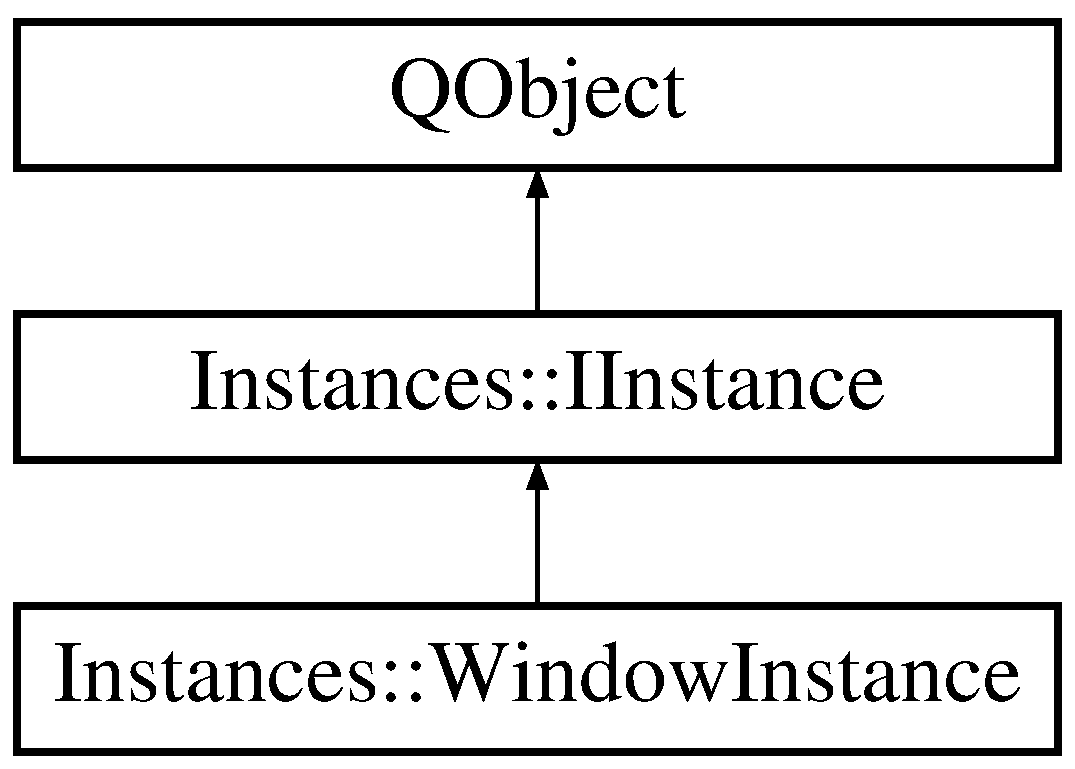
\includegraphics[height=3.000000cm]{classInstances_1_1IInstance}
\end{center}
\end{figure}
\subsection*{Signals}
\begin{DoxyCompactItemize}
\item 
\hypertarget{classInstances_1_1IInstance_aa1981041a376e4c14ebca95df76cb041}{void {\bfseries run\+Code} (\hyperlink{classInstances_1_1IInstance}{I\+Instance} $\ast$)}\label{classInstances_1_1IInstance_aa1981041a376e4c14ebca95df76cb041}

\item 
\hypertarget{classInstances_1_1IInstance_aa2de904201702d2da2fd8fe9776fcfa5}{void {\bfseries stop\+Code} (\hyperlink{classInstances_1_1IInstance}{I\+Instance} $\ast$)}\label{classInstances_1_1IInstance_aa2de904201702d2da2fd8fe9776fcfa5}

\item 
\hypertarget{classInstances_1_1IInstance_acf3c3769af5448b3093e42b73e01c7e6}{void {\bfseries closing} (\hyperlink{classInstances_1_1IInstance}{I\+Instance} $\ast$)}\label{classInstances_1_1IInstance_acf3c3769af5448b3093e42b73e01c7e6}

\item 
\hypertarget{classInstances_1_1IInstance_a6f3b9855e287de954554c631bd7c0a8b}{void {\bfseries close\+All} ()}\label{classInstances_1_1IInstance_a6f3b9855e287de954554c631bd7c0a8b}

\item 
\hypertarget{classInstances_1_1IInstance_aea2d89deb68d4ba6d5833e03ff6a48dc}{void {\bfseries open\+Help} (\hyperlink{classInstances_1_1IInstance}{I\+Instance} $\ast$)}\label{classInstances_1_1IInstance_aea2d89deb68d4ba6d5833e03ff6a48dc}

\item 
\hypertarget{classInstances_1_1IInstance_a1864f99f3c54f539980c3e1a2ab2164d}{void {\bfseries open\+Settings} (\hyperlink{classInstances_1_1IInstance}{I\+Instance} $\ast$)}\label{classInstances_1_1IInstance_a1864f99f3c54f539980c3e1a2ab2164d}

\item 
\hypertarget{classInstances_1_1IInstance_a9ecdadd405b81e04a2b052b30efd6b9f}{void {\bfseries change\+Setting} (\hyperlink{classInstances_1_1IInstance}{I\+Instance} $\ast$, const Q\+String \&key, Q\+Variant value)}\label{classInstances_1_1IInstance_a9ecdadd405b81e04a2b052b30efd6b9f}

\item 
\hypertarget{classInstances_1_1IInstance_a4efdf11046ad14aaa6422dfe6eca761d}{void {\bfseries change\+Settings} (\hyperlink{classInstances_1_1IInstance}{I\+Instance} $\ast$, const Q\+Hash$<$ Q\+String, Q\+Variant $>$ \&)}\label{classInstances_1_1IInstance_a4efdf11046ad14aaa6422dfe6eca761d}

\item 
\hypertarget{classInstances_1_1IInstance_ab5dc40987e611bdc3036d59cf077d0e6}{void {\bfseries get\+Setting} (\hyperlink{classInstances_1_1IInstance}{I\+Instance} $\ast$, const Q\+String \&key, Q\+Variant \&value)}\label{classInstances_1_1IInstance_ab5dc40987e611bdc3036d59cf077d0e6}

\item 
\hypertarget{classInstances_1_1IInstance_a71691d22518c4f60f557c39c44de35b8}{void {\bfseries get\+Settings} (\hyperlink{classInstances_1_1IInstance}{I\+Instance} $\ast$, Q\+Hash$<$ Q\+String, Q\+Variant $>$ \&settings)}\label{classInstances_1_1IInstance_a71691d22518c4f60f557c39c44de35b8}

\end{DoxyCompactItemize}
\subsection*{Public Member Functions}
\begin{DoxyCompactItemize}
\item 
\hypertarget{classInstances_1_1IInstance_aa0e6667c2b463f94edb26976f9fe0e56}{{\bfseries I\+Instance} (int id, Q\+Object $\ast$parent=0)}\label{classInstances_1_1IInstance_aa0e6667c2b463f94edb26976f9fe0e56}

\item 
\hypertarget{classInstances_1_1IInstance_ab45b5dcb803b7fc3de490a76ff359583}{virtual bool {\bfseries close} ()=0}\label{classInstances_1_1IInstance_ab45b5dcb803b7fc3de490a76ff359583}

\item 
\hypertarget{classInstances_1_1IInstance_abea7dafb6274a84bbbc58d07d8bc4072}{virtual void {\bfseries report\+Error} (const Q\+String \&)=0}\label{classInstances_1_1IInstance_abea7dafb6274a84bbbc58d07d8bc4072}

\item 
\hypertarget{classInstances_1_1IInstance_a1eab02bfd1b9acc33172ec95d2861c57}{virtual void {\bfseries report\+Warning} (const Q\+String \&)=0}\label{classInstances_1_1IInstance_a1eab02bfd1b9acc33172ec95d2861c57}

\item 
\hypertarget{classInstances_1_1IInstance_a12f7c89db4f39042b6e19594a54f5587}{virtual void {\bfseries code\+Stopped} ()=0}\label{classInstances_1_1IInstance_a12f7c89db4f39042b6e19594a54f5587}

\item 
\hypertarget{classInstances_1_1IInstance_a8cee5564d63579bcd7b878b7feaed411}{virtual void {\bfseries highlight\+Errored\+Line} (int)=0}\label{classInstances_1_1IInstance_a8cee5564d63579bcd7b878b7feaed411}

\item 
\hypertarget{classInstances_1_1IInstance_a637a26491b9efe024370716d5d295484}{virtual Q\+String {\bfseries source\+Code} () const =0}\label{classInstances_1_1IInstance_a637a26491b9efe024370716d5d295484}

\item 
\hypertarget{classInstances_1_1IInstance_ac13fdb953dda08184f7b9dcab7d0c259}{virtual Q\+String {\bfseries title} () const =0}\label{classInstances_1_1IInstance_ac13fdb953dda08184f7b9dcab7d0c259}

\end{DoxyCompactItemize}
\subsection*{Public Attributes}
\begin{DoxyCompactItemize}
\item 
\hypertarget{classInstances_1_1IInstance_a215b003cb2f0986801fa911533794b14}{const int {\bfseries I\+D}}\label{classInstances_1_1IInstance_a215b003cb2f0986801fa911533794b14}

\end{DoxyCompactItemize}
\subsection*{Protected Member Functions}
\begin{DoxyCompactItemize}
\item 
\hypertarget{classInstances_1_1IInstance_ae508b083261f920a73cf1e72b3e39b60}{\hyperlink{classInstances_1_1IInstance}{I\+Instance} \& {\bfseries operator=} (const \hyperlink{classInstances_1_1IInstance}{I\+Instance} \&rhs)}\label{classInstances_1_1IInstance_ae508b083261f920a73cf1e72b3e39b60}

\item 
\hypertarget{classInstances_1_1IInstance_ae8adfd07ed05a7d1b49d364dd2bd3259}{\hyperlink{classInstances_1_1IInstance}{I\+Instance} \& {\bfseries operator=} (\hyperlink{classInstances_1_1IInstance}{I\+Instance} \&\&rhs)}\label{classInstances_1_1IInstance_ae8adfd07ed05a7d1b49d364dd2bd3259}

\end{DoxyCompactItemize}


\subsection{Detailed Description}
The \hyperlink{classInstances_1_1IInstance}{I\+Instance} class. 

Abstract baseclass from which all instances are derived that are managed by the backend. 

The documentation for this class was generated from the following file\+:\begin{DoxyCompactItemize}
\item 
src/\+Instances/I\+Instance.\+hpp\end{DoxyCompactItemize}

\hypertarget{classLayoutTab}{\section{Layout\+Tab Class Reference}
\label{classLayoutTab}\index{Layout\+Tab@{Layout\+Tab}}
}


The \hyperlink{classLayoutTab}{Layout\+Tab} class.  




{\ttfamily \#include $<$Settings\+Tab.\+hpp$>$}

Inheritance diagram for Layout\+Tab\+:\begin{figure}[H]
\begin{center}
\leavevmode
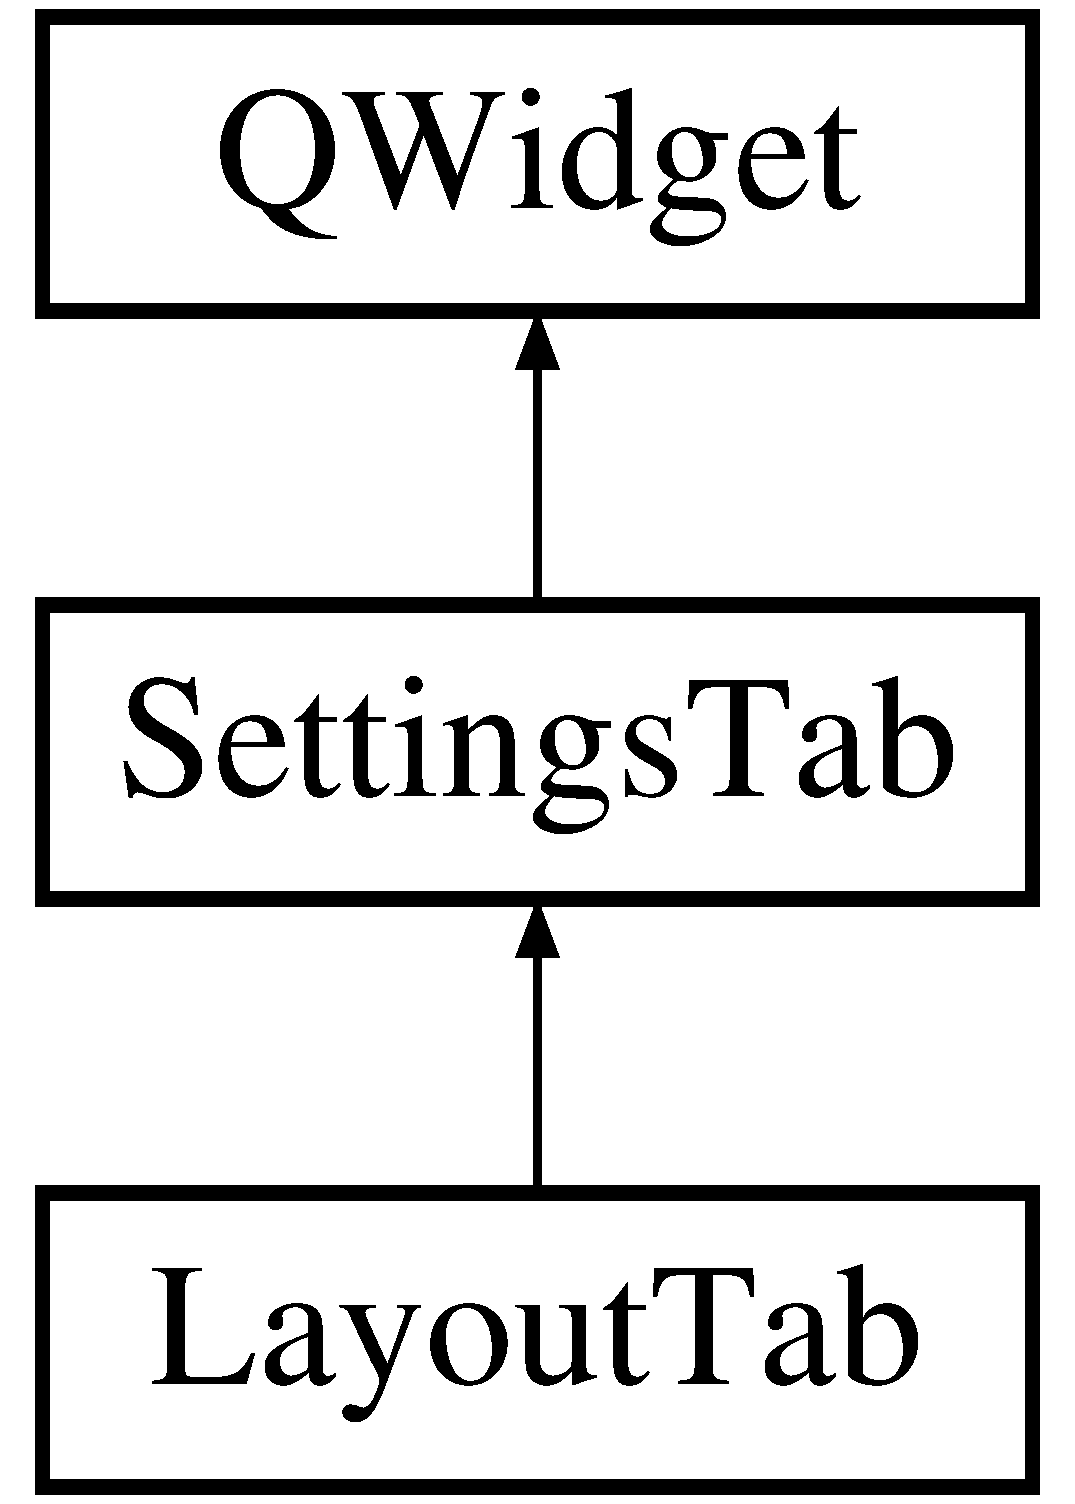
\includegraphics[height=3.000000cm]{classLayoutTab}
\end{center}
\end{figure}
\subsection*{Signals}
\begin{DoxyCompactItemize}
\item 
\hypertarget{classSettingsTab_ab72744b5433a111f3e79da0ef1d9af74}{void {\bfseries content\+Changed} ()}\label{classSettingsTab_ab72744b5433a111f3e79da0ef1d9af74}

\end{DoxyCompactItemize}
\subsection*{Public Member Functions}
\begin{DoxyCompactItemize}
\item 
\hyperlink{classLayoutTab_ad7be4bcefe1444229216a91166d592dc}{Layout\+Tab} (Q\+Hash$<$ Q\+String, Q\+Variant $>$ $\ast$Settings, Q\+Widget $\ast$parent=0)
\begin{DoxyCompactList}\small\item\em \hyperlink{classLayoutTab_ad7be4bcefe1444229216a91166d592dc}{Layout\+Tab\+::\+Layout\+Tab}. \end{DoxyCompactList}\item 
\hyperlink{classLayoutTab_a9801cd1febbd7ce47aa9f0a5863596e9}{$\sim$\+Layout\+Tab} ()
\begin{DoxyCompactList}\small\item\em \hyperlink{classLayoutTab_a9801cd1febbd7ce47aa9f0a5863596e9}{Layout\+Tab\+::$\sim$\+Layout\+Tab}. \end{DoxyCompactList}\end{DoxyCompactItemize}
\subsection*{Protected Attributes}
\begin{DoxyCompactItemize}
\item 
\hypertarget{classSettingsTab_af6d39f524ae1d31aa8655c1957939287}{Q\+Hash$<$ Q\+String, Q\+Variant $>$ $\ast$ {\bfseries settings}}\label{classSettingsTab_af6d39f524ae1d31aa8655c1957939287}

\end{DoxyCompactItemize}


\subsection{Detailed Description}
The \hyperlink{classLayoutTab}{Layout\+Tab} class. 

\begin{DoxyAuthor}{Author}
Veit Heller(s0539501) \& Tobias Brosge(s0539713)
\end{DoxyAuthor}
A subclass of \hyperlink{classSettingsTab}{Settings\+Tab} that implements one of the tabs of the \hyperlink{classSettingsWindow}{Settings\+Window} in which all configurations regarding layout can be found. 

\subsection{Constructor \& Destructor Documentation}
\hypertarget{classLayoutTab_ad7be4bcefe1444229216a91166d592dc}{\index{Layout\+Tab@{Layout\+Tab}!Layout\+Tab@{Layout\+Tab}}
\index{Layout\+Tab@{Layout\+Tab}!Layout\+Tab@{Layout\+Tab}}
\subsubsection[{Layout\+Tab}]{\setlength{\rightskip}{0pt plus 5cm}Layout\+Tab\+::\+Layout\+Tab (
\begin{DoxyParamCaption}
\item[{Q\+Hash$<$ Q\+String, Q\+Variant $>$ $\ast$}]{Settings, }
\item[{Q\+Widget $\ast$}]{parent = {\ttfamily 0}}
\end{DoxyParamCaption}
)}}\label{classLayoutTab_ad7be4bcefe1444229216a91166d592dc}


\hyperlink{classLayoutTab_ad7be4bcefe1444229216a91166d592dc}{Layout\+Tab\+::\+Layout\+Tab}. 

Constructor of the \hyperlink{classLayoutTab}{Layout\+Tab} class. Calls the add\+Layout member function. \hypertarget{classLayoutTab_a9801cd1febbd7ce47aa9f0a5863596e9}{\index{Layout\+Tab@{Layout\+Tab}!````~Layout\+Tab@{$\sim$\+Layout\+Tab}}
\index{````~Layout\+Tab@{$\sim$\+Layout\+Tab}!Layout\+Tab@{Layout\+Tab}}
\subsubsection[{$\sim$\+Layout\+Tab}]{\setlength{\rightskip}{0pt plus 5cm}Layout\+Tab\+::$\sim$\+Layout\+Tab (
\begin{DoxyParamCaption}
{}
\end{DoxyParamCaption}
)}}\label{classLayoutTab_a9801cd1febbd7ce47aa9f0a5863596e9}


\hyperlink{classLayoutTab_a9801cd1febbd7ce47aa9f0a5863596e9}{Layout\+Tab\+::$\sim$\+Layout\+Tab}. 

Destructor of the \hyperlink{classLayoutTab}{Layout\+Tab} class. Deletes the G\+U\+I elements. 

The documentation for this class was generated from the following files\+:\begin{DoxyCompactItemize}
\item 
src/Settings\+Tab.\+hpp\item 
src/Settings\+Tab.\+cpp\end{DoxyCompactItemize}

\hypertarget{classLineHighlighting}{\section{Line\+Highlighting Class Reference}
\label{classLineHighlighting}\index{Line\+Highlighting@{Line\+Highlighting}}
}


The \hyperlink{classLineHighlighting}{Line\+Highlighting} helper class.  




{\ttfamily \#include $<$Code\+Editor.\+hpp$>$}

Inheritance diagram for Line\+Highlighting\+:\begin{figure}[H]
\begin{center}
\leavevmode
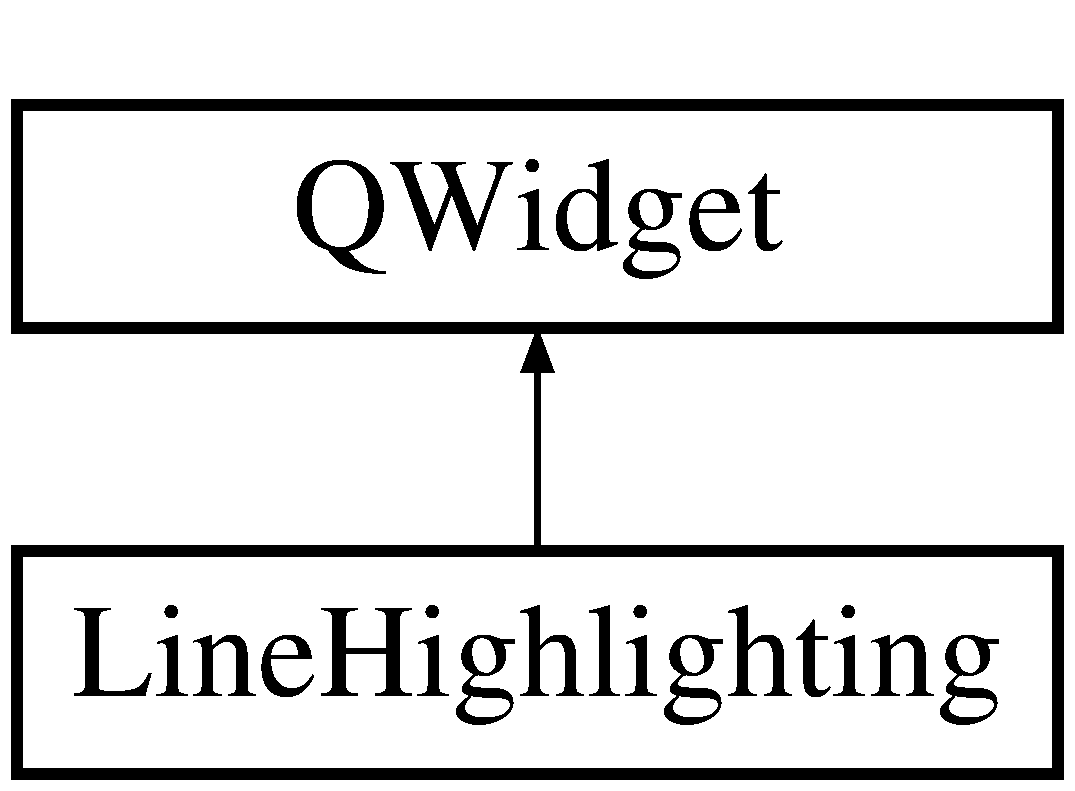
\includegraphics[height=2.000000cm]{classLineHighlighting}
\end{center}
\end{figure}
\subsection*{Public Member Functions}
\begin{DoxyCompactItemize}
\item 
\hypertarget{classLineHighlighting_ae54cb1a71e7aff9e91fe41a642b674a6}{{\bfseries Line\+Highlighting} (\hyperlink{classCodeEditor}{Code\+Editor} $\ast$editor)}\label{classLineHighlighting_ae54cb1a71e7aff9e91fe41a642b674a6}

\item 
\hypertarget{classLineHighlighting_a125e4c4fb6f09b82ef1617ed9d6c936a}{virtual Q\+Size {\bfseries size\+Hint} () const }\label{classLineHighlighting_a125e4c4fb6f09b82ef1617ed9d6c936a}

\end{DoxyCompactItemize}
\subsection*{Protected Member Functions}
\begin{DoxyCompactItemize}
\item 
\hypertarget{classLineHighlighting_a14c16b62a7220a72288dc68b0b3ce42c}{virtual void {\bfseries paint\+Event} (Q\+Paint\+Event $\ast$event)}\label{classLineHighlighting_a14c16b62a7220a72288dc68b0b3ce42c}

\end{DoxyCompactItemize}


\subsection{Detailed Description}
The \hyperlink{classLineHighlighting}{Line\+Highlighting} helper class. 

\begin{DoxyAuthor}{Author}
Veit Heller(s0539501) \& Tobias Brosge(s0539713)
\end{DoxyAuthor}
A helping subclass of Q\+Widget for the code\+Editor that is responsible for highlighting the current line. 

The documentation for this class was generated from the following file\+:\begin{DoxyCompactItemize}
\item 
src/Code\+Editor.\+hpp\end{DoxyCompactItemize}

\hypertarget{classLiveThread}{\section{Live\+Thread Class Reference}
\label{classLiveThread}\index{Live\+Thread@{Live\+Thread}}
}


The \hyperlink{classLiveThread}{Live\+Thread} class.  




{\ttfamily \#include $<$Live\+Thread.\+hpp$>$}

Inheritance diagram for Live\+Thread\+:\begin{figure}[H]
\begin{center}
\leavevmode
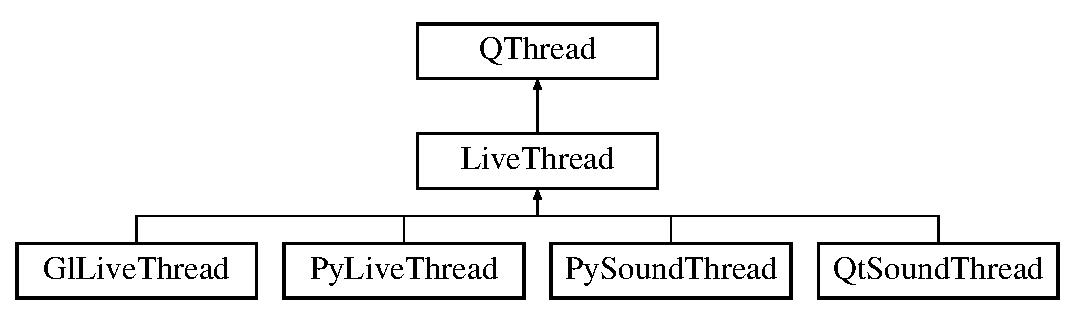
\includegraphics[height=3.000000cm]{classLiveThread}
\end{center}
\end{figure}
\subsection*{Public Member Functions}
\begin{DoxyCompactItemize}
\item 
\hypertarget{classLiveThread_ae6d3dbf7a848c4c45c6792f7b6dd0ba1}{{\bfseries Live\+Thread} (const long identity, Q\+Object $\ast$parent=0)}\label{classLiveThread_ae6d3dbf7a848c4c45c6792f7b6dd0ba1}

\item 
\hypertarget{classLiveThread_ac3fa286fc1a4cd6482f66b490301431d}{virtual void {\bfseries run} ()=0}\label{classLiveThread_ac3fa286fc1a4cd6482f66b490301431d}

\item 
\hypertarget{classLiveThread_a7057545ae0d705fa19368d8c8e064bc8}{virtual void {\bfseries initialize} (const Q\+String \&title, const Q\+String \&instructions)=0}\label{classLiveThread_a7057545ae0d705fa19368d8c8e064bc8}

\item 
\hypertarget{classLiveThread_a03674124c426aa2f40a0e704100a5ae6}{virtual bool {\bfseries update\+Code} (const Q\+String \&title, const Q\+String \&instructions)=0}\label{classLiveThread_a03674124c426aa2f40a0e704100a5ae6}

\end{DoxyCompactItemize}
\subsection*{Public Attributes}
\begin{DoxyCompactItemize}
\item 
\hypertarget{classLiveThread_a5cfdefd7574fb1f34bbe1d21b5e3c1d8}{const long {\bfseries I\+D}}\label{classLiveThread_a5cfdefd7574fb1f34bbe1d21b5e3c1d8}

\end{DoxyCompactItemize}


\subsection{Detailed Description}
The \hyperlink{classLiveThread}{Live\+Thread} class. 

A subclass of Q\+Thread that is optimized for running the interpreters we need. 

The documentation for this class was generated from the following file\+:\begin{DoxyCompactItemize}
\item 
src/Live\+Thread.\+hpp\end{DoxyCompactItemize}

\hypertarget{classPyLiveInterpreter}{\section{Py\+Live\+Interpreter Class Reference}
\label{classPyLiveInterpreter}\index{Py\+Live\+Interpreter@{Py\+Live\+Interpreter}}
}


The \hyperlink{classPyLiveInterpreter}{Py\+Live\+Interpreter} class.  




{\ttfamily \#include $<$Py\+Live\+Interpreter.\+hpp$>$}

Inheritance diagram for Py\+Live\+Interpreter\+:\begin{figure}[H]
\begin{center}
\leavevmode
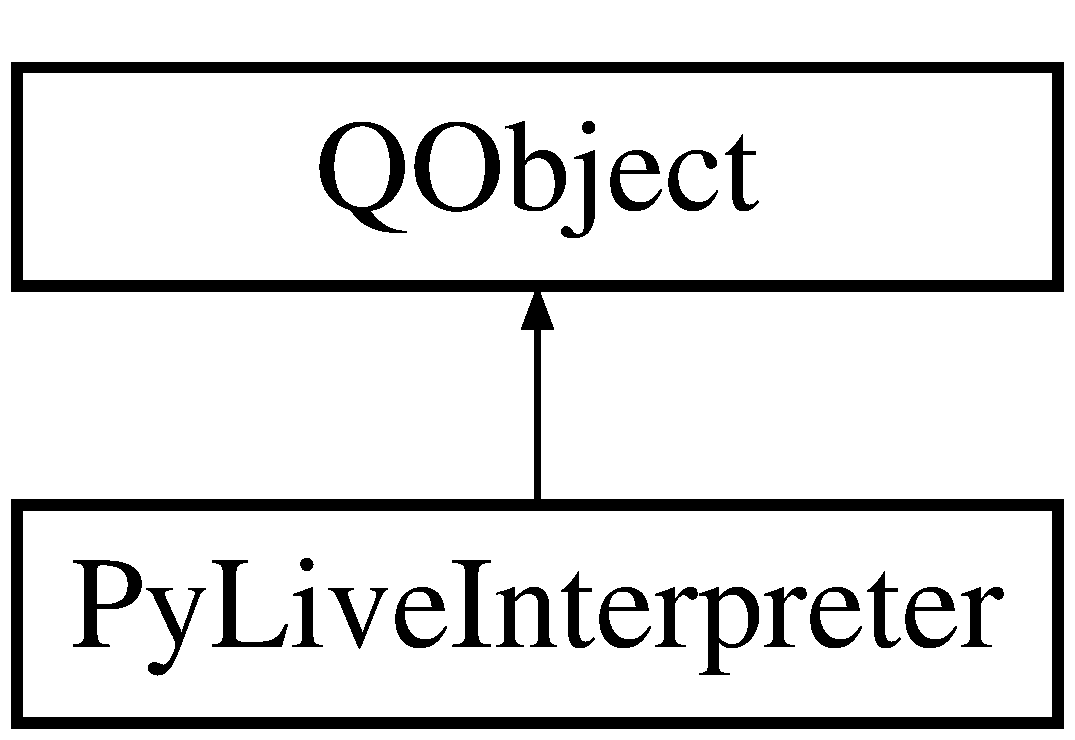
\includegraphics[height=2.000000cm]{classPyLiveInterpreter}
\end{center}
\end{figure}
\subsection*{Signals}
\begin{DoxyCompactItemize}
\item 
\hypertarget{classPyLiveInterpreter_a4571972ede3e0fb04f6eaf1720acae5c}{void {\bfseries done\+Signal} (Q\+String, int)}\label{classPyLiveInterpreter_a4571972ede3e0fb04f6eaf1720acae5c}

\end{DoxyCompactItemize}
\subsection*{Public Member Functions}
\begin{DoxyCompactItemize}
\item 
\hyperlink{classPyLiveInterpreter_a1781393242e987a75f549d59531db321}{Py\+Live\+Interpreter} (char $\ast$, char $\ast$)
\begin{DoxyCompactList}\small\item\em \hyperlink{classPyLiveInterpreter_a1781393242e987a75f549d59531db321}{Py\+Live\+Interpreter\+::\+Py\+Live\+Interpreter}. \end{DoxyCompactList}\item 
void \hyperlink{classPyLiveInterpreter_a8570e8a6c3726d450fd2fb5f74a86461}{run} ()
\begin{DoxyCompactList}\small\item\em \hyperlink{classPyLiveInterpreter_a8570e8a6c3726d450fd2fb5f74a86461}{Py\+Live\+Interpreter\+::run}. \end{DoxyCompactList}\item 
bool \hyperlink{classPyLiveInterpreter_ab02b4ef045b07140fae048295ef336b8}{update\+Code} (Q\+String, Q\+String)
\begin{DoxyCompactList}\small\item\em \hyperlink{classPyLiveInterpreter_ab02b4ef045b07140fae048295ef336b8}{Py\+Live\+Interpreter\+::update\+Code}. \end{DoxyCompactList}\item 
\hyperlink{classPyLiveInterpreter_a400b3e1ed26b84937c7e8738191942e0}{$\sim$\+Py\+Live\+Interpreter} ()
\begin{DoxyCompactList}\small\item\em \hyperlink{classPyLiveInterpreter_a400b3e1ed26b84937c7e8738191942e0}{Py\+Live\+Interpreter\+::$\sim$\+Py\+Live\+Interpreter}. \end{DoxyCompactList}\end{DoxyCompactItemize}


\subsection{Detailed Description}
The \hyperlink{classPyLiveInterpreter}{Py\+Live\+Interpreter} class. 

A subclass of Q\+Thread that implements an environment for python coding while keeping the main codeeditor thread clean by dispatching. 

\subsection{Constructor \& Destructor Documentation}
\hypertarget{classPyLiveInterpreter_a1781393242e987a75f549d59531db321}{\index{Py\+Live\+Interpreter@{Py\+Live\+Interpreter}!Py\+Live\+Interpreter@{Py\+Live\+Interpreter}}
\index{Py\+Live\+Interpreter@{Py\+Live\+Interpreter}!Py\+Live\+Interpreter@{Py\+Live\+Interpreter}}
\subsubsection[{Py\+Live\+Interpreter}]{\setlength{\rightskip}{0pt plus 5cm}Py\+Live\+Interpreter\+::\+Py\+Live\+Interpreter (
\begin{DoxyParamCaption}
\item[{char $\ast$}]{prog\+Name, }
\item[{char $\ast$}]{py\+Instructions}
\end{DoxyParamCaption}
)}}\label{classPyLiveInterpreter_a1781393242e987a75f549d59531db321}


\hyperlink{classPyLiveInterpreter_a1781393242e987a75f549d59531db321}{Py\+Live\+Interpreter\+::\+Py\+Live\+Interpreter}. 


\begin{DoxyParams}{Parameters}
{\em prog\+Name} & \\
\hline
{\em py\+Instructions} & The constructor of the Py\+Live\+Interpreterclass. Sets up the python interpreter, the instructions with which it will be fed, the class variables and the break shortcut. \\
\hline
\end{DoxyParams}
\hypertarget{classPyLiveInterpreter_a400b3e1ed26b84937c7e8738191942e0}{\index{Py\+Live\+Interpreter@{Py\+Live\+Interpreter}!````~Py\+Live\+Interpreter@{$\sim$\+Py\+Live\+Interpreter}}
\index{````~Py\+Live\+Interpreter@{$\sim$\+Py\+Live\+Interpreter}!Py\+Live\+Interpreter@{Py\+Live\+Interpreter}}
\subsubsection[{$\sim$\+Py\+Live\+Interpreter}]{\setlength{\rightskip}{0pt plus 5cm}Py\+Live\+Interpreter\+::$\sim$\+Py\+Live\+Interpreter (
\begin{DoxyParamCaption}
{}
\end{DoxyParamCaption}
)}}\label{classPyLiveInterpreter_a400b3e1ed26b84937c7e8738191942e0}


\hyperlink{classPyLiveInterpreter_a400b3e1ed26b84937c7e8738191942e0}{Py\+Live\+Interpreter\+::$\sim$\+Py\+Live\+Interpreter}. 

The destructor of the \hyperlink{classPyLiveInterpreter}{Py\+Live\+Interpreter} class. Kills the python interpreter. 

\subsection{Member Function Documentation}
\hypertarget{classPyLiveInterpreter_a8570e8a6c3726d450fd2fb5f74a86461}{\index{Py\+Live\+Interpreter@{Py\+Live\+Interpreter}!run@{run}}
\index{run@{run}!Py\+Live\+Interpreter@{Py\+Live\+Interpreter}}
\subsubsection[{run}]{\setlength{\rightskip}{0pt plus 5cm}void Py\+Live\+Interpreter\+::run (
\begin{DoxyParamCaption}
{}
\end{DoxyParamCaption}
)}}\label{classPyLiveInterpreter_a8570e8a6c3726d450fd2fb5f74a86461}


\hyperlink{classPyLiveInterpreter_a8570e8a6c3726d450fd2fb5f74a86461}{Py\+Live\+Interpreter\+::run}. 

The main loop. Calls the user code executing method and Q\+\_\+\+E\+M\+I\+Ts a signal when it's done. \hypertarget{classPyLiveInterpreter_ab02b4ef045b07140fae048295ef336b8}{\index{Py\+Live\+Interpreter@{Py\+Live\+Interpreter}!update\+Code@{update\+Code}}
\index{update\+Code@{update\+Code}!Py\+Live\+Interpreter@{Py\+Live\+Interpreter}}
\subsubsection[{update\+Code}]{\setlength{\rightskip}{0pt plus 5cm}bool Py\+Live\+Interpreter\+::update\+Code (
\begin{DoxyParamCaption}
\item[{Q\+String}]{filename, }
\item[{Q\+String}]{instructions}
\end{DoxyParamCaption}
)}}\label{classPyLiveInterpreter_ab02b4ef045b07140fae048295ef336b8}


\hyperlink{classPyLiveInterpreter_ab02b4ef045b07140fae048295ef336b8}{Py\+Live\+Interpreter\+::update\+Code}. 


\begin{DoxyParams}{Parameters}
{\em filename} & \\
\hline
{\em instructions} & \\
\hline
\end{DoxyParams}
\begin{DoxyReturn}{Returns}
true if the name of the program could be changed, false otherwise
\end{DoxyReturn}
Updates the code of the currently running Python interpreter. 

The documentation for this class was generated from the following files\+:\begin{DoxyCompactItemize}
\item 
src/Py\+Live\+Interpreter.\+hpp\item 
src/Py\+Live\+Interpreter.\+cpp\end{DoxyCompactItemize}

\hypertarget{classPyLiveThread}{\section{Py\+Live\+Thread Class Reference}
\label{classPyLiveThread}\index{Py\+Live\+Thread@{Py\+Live\+Thread}}
}
Inheritance diagram for Py\+Live\+Thread\+:\begin{figure}[H]
\begin{center}
\leavevmode
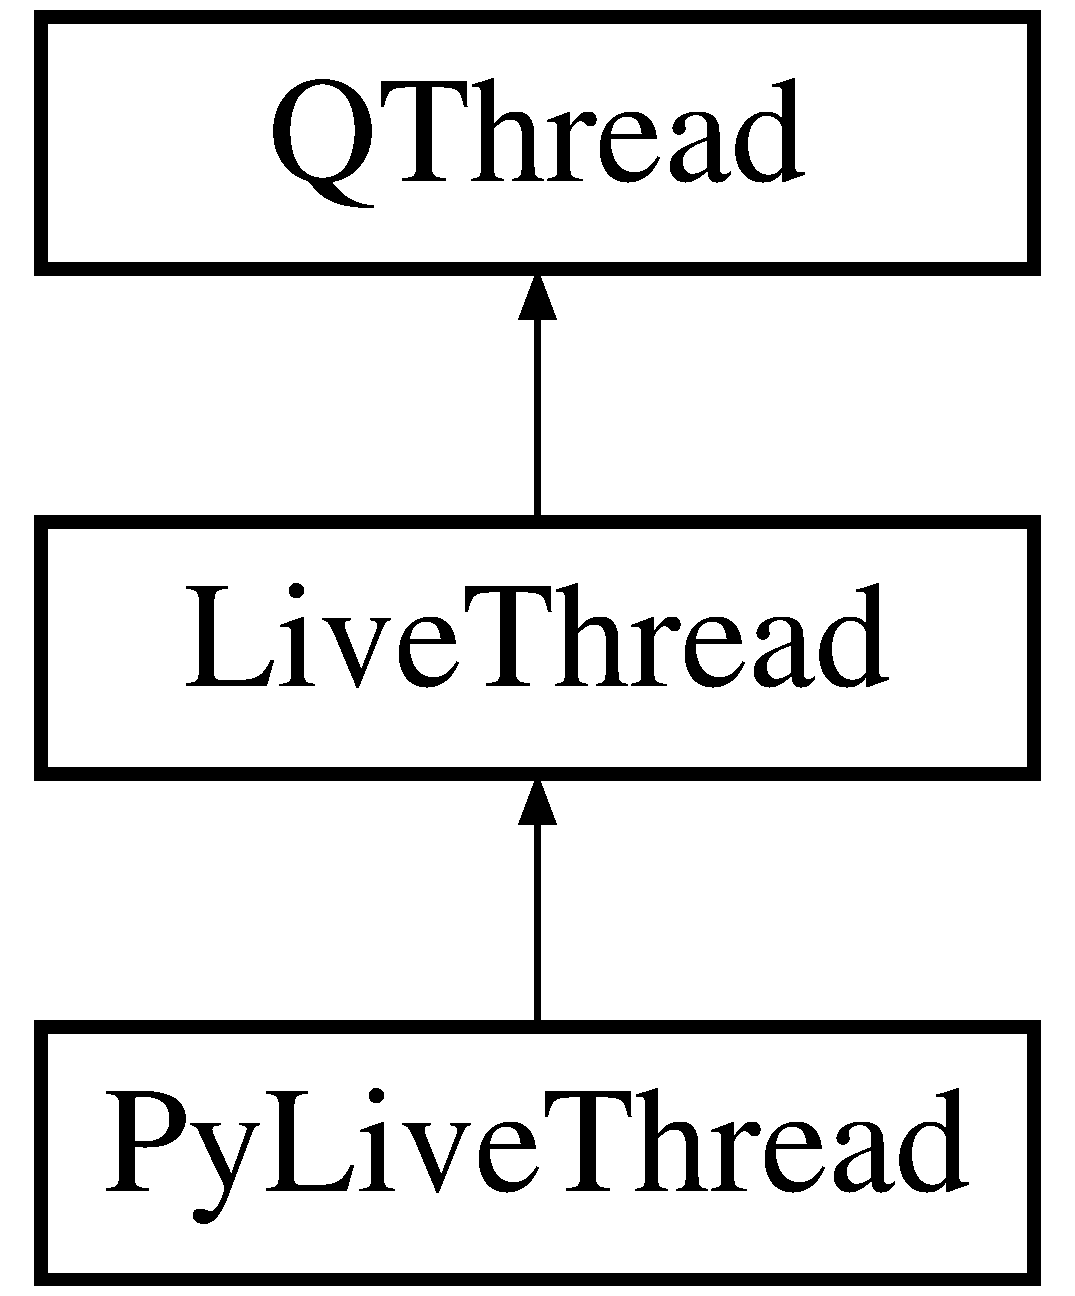
\includegraphics[height=3.000000cm]{classPyLiveThread}
\end{center}
\end{figure}
\subsection*{Public Slots}
\begin{DoxyCompactItemize}
\item 
\hypertarget{classPyLiveThread_a8f112d05d5eae7a756f3e60e4fe777b0}{void {\bfseries done\+Signal\+Received} (Q\+String exception, int lineno)}\label{classPyLiveThread_a8f112d05d5eae7a756f3e60e4fe777b0}

\end{DoxyCompactItemize}
\subsection*{Signals}
\begin{DoxyCompactItemize}
\item 
\hypertarget{classPyLiveThread_a2f8fffefb6729d062f6c03d716435c67}{void {\bfseries done\+Signal} (\hyperlink{classPyLiveThread}{Py\+Live\+Thread} $\ast$, Q\+String, int)}\label{classPyLiveThread_a2f8fffefb6729d062f6c03d716435c67}

\end{DoxyCompactItemize}
\subsection*{Public Member Functions}
\begin{DoxyCompactItemize}
\item 
\hypertarget{classPyLiveThread_a1a20ad7d1594c37d9651e2971f5df803}{{\bfseries Py\+Live\+Thread} (const long identity, Q\+Object $\ast$parent=0)}\label{classPyLiveThread_a1a20ad7d1594c37d9651e2971f5df803}

\item 
\hypertarget{classPyLiveThread_a03bd9e5eba5ede6530221307e432bef1}{void {\bfseries run} () Q\+\_\+\+D\+E\+C\+L\+\_\+\+O\+V\+E\+R\+R\+I\+D\+E}\label{classPyLiveThread_a03bd9e5eba5ede6530221307e432bef1}

\item 
\hypertarget{classPyLiveThread_ad4f6dcdcab25b029c311bed78fa5fd92}{void {\bfseries initialize} (const Q\+String \&title, const Q\+String \&instructions)}\label{classPyLiveThread_ad4f6dcdcab25b029c311bed78fa5fd92}

\item 
\hypertarget{classPyLiveThread_a212b2b893d60e2ff898d1b0661987eef}{bool {\bfseries update\+Code} (const Q\+String \&filename, const Q\+String \&code)}\label{classPyLiveThread_a212b2b893d60e2ff898d1b0661987eef}

\end{DoxyCompactItemize}
\subsection*{Public Attributes}
\begin{DoxyCompactItemize}
\item 
\hypertarget{classLiveThread_a5cfdefd7574fb1f34bbe1d21b5e3c1d8}{const long {\bfseries I\+D}}\label{classLiveThread_a5cfdefd7574fb1f34bbe1d21b5e3c1d8}

\end{DoxyCompactItemize}


The documentation for this class was generated from the following file\+:\begin{DoxyCompactItemize}
\item 
src/Live\+Thread.\+hpp\end{DoxyCompactItemize}

\hypertarget{classPySoundGenerator}{\section{Py\+Sound\+Generator Class Reference}
\label{classPySoundGenerator}\index{Py\+Sound\+Generator@{Py\+Sound\+Generator}}
}


The \hyperlink{classPySoundGenerator}{Py\+Sound\+Generator} class.  




{\ttfamily \#include $<$Py\+Sound\+Generator.\+hpp$>$}

Inheritance diagram for Py\+Sound\+Generator\+:\begin{figure}[H]
\begin{center}
\leavevmode
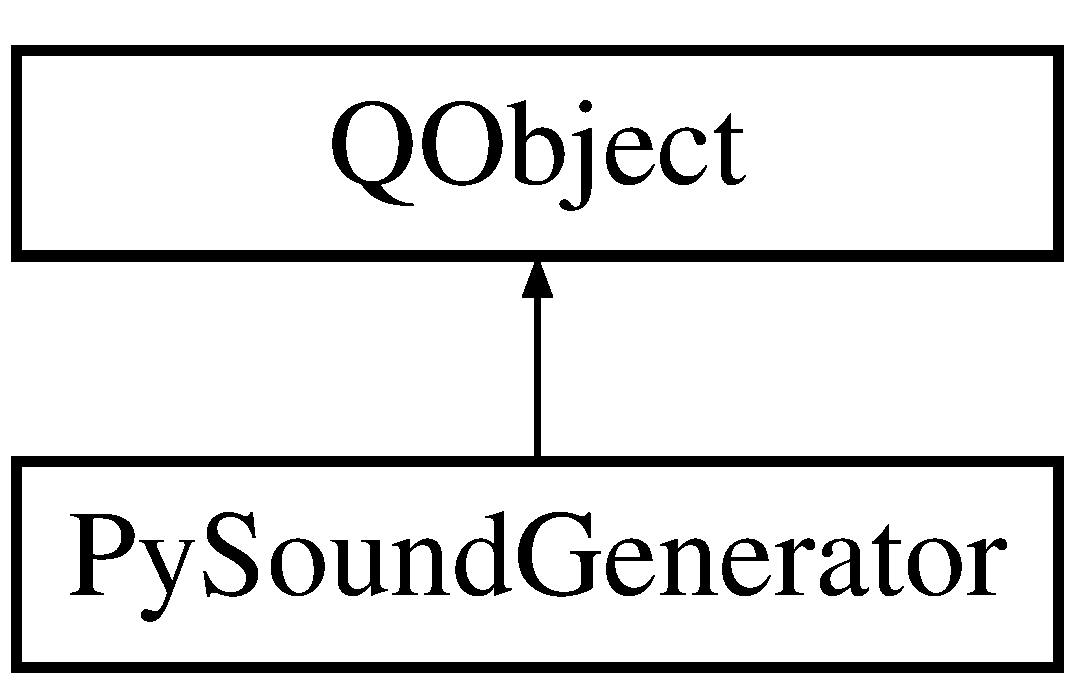
\includegraphics[height=2.000000cm]{classPySoundGenerator}
\end{center}
\end{figure}
\subsection*{Signals}
\begin{DoxyCompactItemize}
\item 
\hypertarget{classPySoundGenerator_a65289c7a550fec38c31c98771a626935}{void {\bfseries done\+Signal} (Q\+String, int)}\label{classPySoundGenerator_a65289c7a550fec38c31c98771a626935}

\end{DoxyCompactItemize}
\subsection*{Public Member Functions}
\begin{DoxyCompactItemize}
\item 
\hyperlink{classPySoundGenerator_a6a39079f1420a4160c9556ca25f136dc}{Py\+Sound\+Generator} (char $\ast$, char $\ast$)
\begin{DoxyCompactList}\small\item\em \hyperlink{classPySoundGenerator_a6a39079f1420a4160c9556ca25f136dc}{Py\+Sound\+Generator\+::\+Py\+Sound\+Generator}. \end{DoxyCompactList}\item 
void \hyperlink{classPySoundGenerator_acfd10c83de4bff94c8a46710d918a7e9}{run} ()
\begin{DoxyCompactList}\small\item\em \hyperlink{classPySoundGenerator_acfd10c83de4bff94c8a46710d918a7e9}{Py\+Sound\+Generator\+::run}. \end{DoxyCompactList}\item 
bool \hyperlink{classPySoundGenerator_a1e45078f4f0b740c849d0c927fa929f1}{update\+Code} (Q\+String, Q\+String)
\begin{DoxyCompactList}\small\item\em \hyperlink{classPySoundGenerator_a1e45078f4f0b740c849d0c927fa929f1}{Py\+Sound\+Generator\+::update\+Code}. \end{DoxyCompactList}\item 
\hyperlink{classPySoundGenerator_aeff90baafa85e12589195ce8206426bf}{$\sim$\+Py\+Sound\+Generator} ()
\begin{DoxyCompactList}\small\item\em \hyperlink{classPySoundGenerator_aeff90baafa85e12589195ce8206426bf}{Py\+Sound\+Generator\+::$\sim$\+Py\+Sound\+Generator}. \end{DoxyCompactList}\end{DoxyCompactItemize}


\subsection{Detailed Description}
The \hyperlink{classPySoundGenerator}{Py\+Sound\+Generator} class. 

\begin{DoxyAuthor}{Author}
Veit Heller(s0539501) \& Tobias Brosge(s0539713)
\end{DoxyAuthor}
A subclass of Q\+Thread that implements an environment for sound live coding while keeping the main codeeditor thread clean by dispatching. Python-\/based. 

\subsection{Constructor \& Destructor Documentation}
\hypertarget{classPySoundGenerator_a6a39079f1420a4160c9556ca25f136dc}{\index{Py\+Sound\+Generator@{Py\+Sound\+Generator}!Py\+Sound\+Generator@{Py\+Sound\+Generator}}
\index{Py\+Sound\+Generator@{Py\+Sound\+Generator}!Py\+Sound\+Generator@{Py\+Sound\+Generator}}
\subsubsection[{Py\+Sound\+Generator}]{\setlength{\rightskip}{0pt plus 5cm}Py\+Sound\+Generator\+::\+Py\+Sound\+Generator (
\begin{DoxyParamCaption}
\item[{char $\ast$}]{prog\+Name, }
\item[{char $\ast$}]{py\+Instructions}
\end{DoxyParamCaption}
)}}\label{classPySoundGenerator_a6a39079f1420a4160c9556ca25f136dc}


\hyperlink{classPySoundGenerator_a6a39079f1420a4160c9556ca25f136dc}{Py\+Sound\+Generator\+::\+Py\+Sound\+Generator}. 


\begin{DoxyParams}{Parameters}
{\em prog\+Name} & \\
\hline
{\em py\+Instructions} & The constructor of the Py\+Sound\+Generatorclass. Sets up the python interpreter, the instructions with which it will be fed, the class variables and the break shortcut. \\
\hline
\end{DoxyParams}
\hypertarget{classPySoundGenerator_aeff90baafa85e12589195ce8206426bf}{\index{Py\+Sound\+Generator@{Py\+Sound\+Generator}!````~Py\+Sound\+Generator@{$\sim$\+Py\+Sound\+Generator}}
\index{````~Py\+Sound\+Generator@{$\sim$\+Py\+Sound\+Generator}!Py\+Sound\+Generator@{Py\+Sound\+Generator}}
\subsubsection[{$\sim$\+Py\+Sound\+Generator}]{\setlength{\rightskip}{0pt plus 5cm}Py\+Sound\+Generator\+::$\sim$\+Py\+Sound\+Generator (
\begin{DoxyParamCaption}
{}
\end{DoxyParamCaption}
)}}\label{classPySoundGenerator_aeff90baafa85e12589195ce8206426bf}


\hyperlink{classPySoundGenerator_aeff90baafa85e12589195ce8206426bf}{Py\+Sound\+Generator\+::$\sim$\+Py\+Sound\+Generator}. 

The destructor of the \hyperlink{classPySoundGenerator}{Py\+Sound\+Generator} class. Kills the python interpreter. 

\subsection{Member Function Documentation}
\hypertarget{classPySoundGenerator_acfd10c83de4bff94c8a46710d918a7e9}{\index{Py\+Sound\+Generator@{Py\+Sound\+Generator}!run@{run}}
\index{run@{run}!Py\+Sound\+Generator@{Py\+Sound\+Generator}}
\subsubsection[{run}]{\setlength{\rightskip}{0pt plus 5cm}void Py\+Sound\+Generator\+::run (
\begin{DoxyParamCaption}
{}
\end{DoxyParamCaption}
)}}\label{classPySoundGenerator_acfd10c83de4bff94c8a46710d918a7e9}


\hyperlink{classPySoundGenerator_acfd10c83de4bff94c8a46710d918a7e9}{Py\+Sound\+Generator\+::run}. 

The main loop. Calls the user code executing method and Q\+\_\+\+E\+M\+I\+Ts a signal when it's done. \hypertarget{classPySoundGenerator_a1e45078f4f0b740c849d0c927fa929f1}{\index{Py\+Sound\+Generator@{Py\+Sound\+Generator}!update\+Code@{update\+Code}}
\index{update\+Code@{update\+Code}!Py\+Sound\+Generator@{Py\+Sound\+Generator}}
\subsubsection[{update\+Code}]{\setlength{\rightskip}{0pt plus 5cm}bool Py\+Sound\+Generator\+::update\+Code (
\begin{DoxyParamCaption}
\item[{Q\+String}]{filename, }
\item[{Q\+String}]{instructions}
\end{DoxyParamCaption}
)}}\label{classPySoundGenerator_a1e45078f4f0b740c849d0c927fa929f1}


\hyperlink{classPySoundGenerator_a1e45078f4f0b740c849d0c927fa929f1}{Py\+Sound\+Generator\+::update\+Code}. 


\begin{DoxyParams}{Parameters}
{\em filename} & \\
\hline
{\em instructions} & \\
\hline
\end{DoxyParams}
\begin{DoxyReturn}{Returns}
true if the name of the program could be changed, false otherwise
\end{DoxyReturn}
Updates the code of the currently running Python interpreter. 

The documentation for this class was generated from the following files\+:\begin{DoxyCompactItemize}
\item 
src/Py\+Sound\+Generator.\+hpp\item 
src/Py\+Sound\+Generator.\+cpp\end{DoxyCompactItemize}

\hypertarget{classPySoundThread}{\section{Py\+Sound\+Thread Class Reference}
\label{classPySoundThread}\index{Py\+Sound\+Thread@{Py\+Sound\+Thread}}
}
Inheritance diagram for Py\+Sound\+Thread\+:\begin{figure}[H]
\begin{center}
\leavevmode
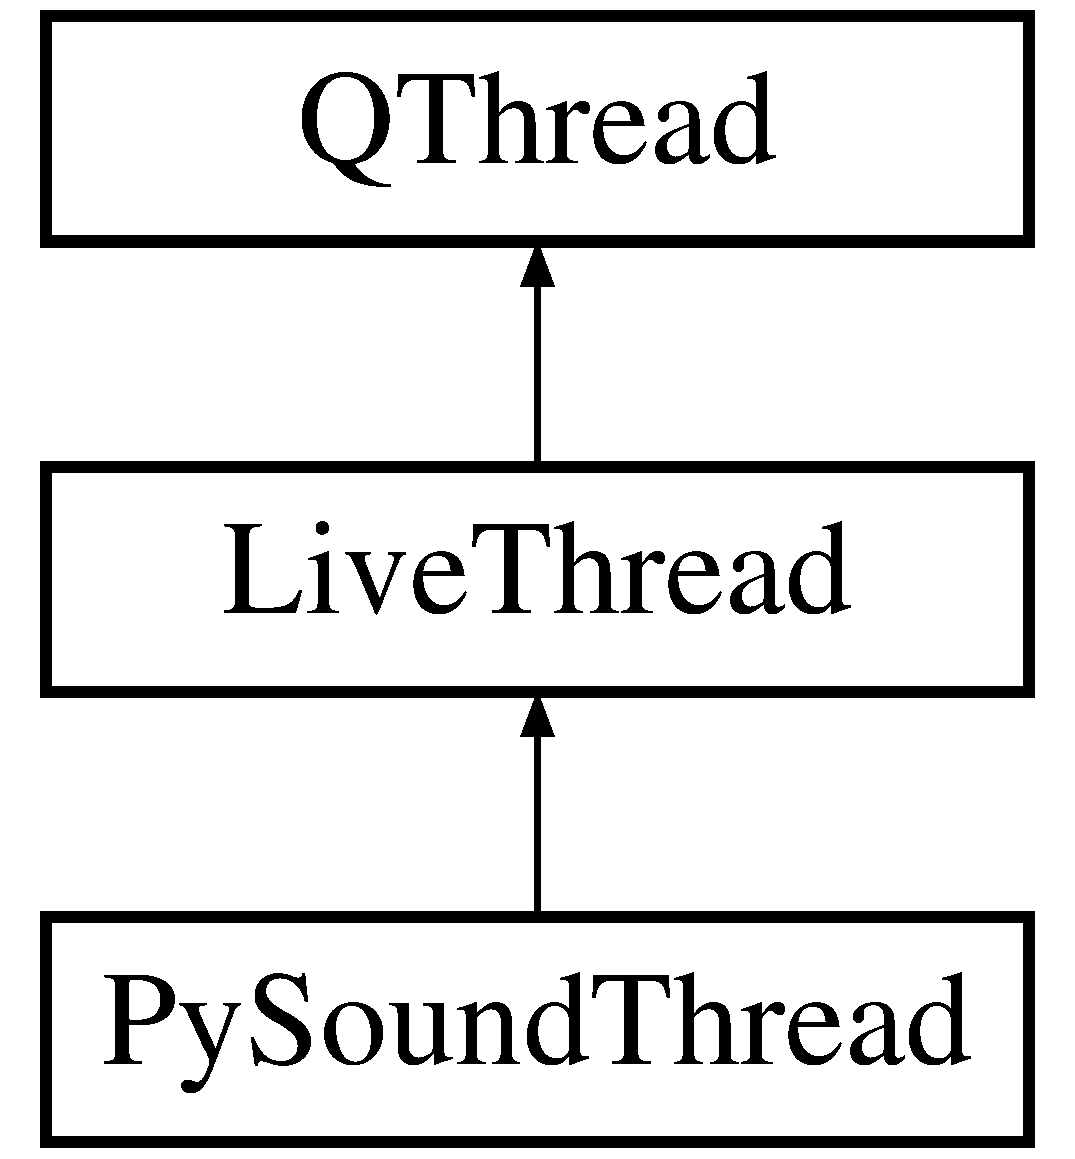
\includegraphics[height=3.000000cm]{classPySoundThread}
\end{center}
\end{figure}
\subsection*{Public Slots}
\begin{DoxyCompactItemize}
\item 
\hypertarget{classPySoundThread_ab840a95275e20cb439369b63612c59cd}{void {\bfseries done\+Signal\+Received} (Q\+String exception, int lineno)}\label{classPySoundThread_ab840a95275e20cb439369b63612c59cd}

\end{DoxyCompactItemize}
\subsection*{Signals}
\begin{DoxyCompactItemize}
\item 
\hypertarget{classPySoundThread_abe6c1331f19a2e74ab586058a1d7f539}{void {\bfseries done\+Signal} (\hyperlink{classPySoundThread}{Py\+Sound\+Thread} $\ast$, Q\+String, int)}\label{classPySoundThread_abe6c1331f19a2e74ab586058a1d7f539}

\end{DoxyCompactItemize}
\subsection*{Public Member Functions}
\begin{DoxyCompactItemize}
\item 
\hypertarget{classPySoundThread_a6243cc4a5d70c97513a1f1e7683347a8}{{\bfseries Py\+Sound\+Thread} (const long identity, Q\+Object $\ast$parent=0)}\label{classPySoundThread_a6243cc4a5d70c97513a1f1e7683347a8}

\item 
\hypertarget{classPySoundThread_afc271219d486efb5557ece0bd5052121}{void {\bfseries run} () Q\+\_\+\+D\+E\+C\+L\+\_\+\+O\+V\+E\+R\+R\+I\+D\+E}\label{classPySoundThread_afc271219d486efb5557ece0bd5052121}

\item 
\hypertarget{classPySoundThread_aa219cc232ef741f992a2ef7ad4a16f88}{void {\bfseries initialize} (const Q\+String \&, const Q\+String \&)}\label{classPySoundThread_aa219cc232ef741f992a2ef7ad4a16f88}

\item 
\hypertarget{classPySoundThread_a90c17718086b36592bc16d005d651390}{bool {\bfseries update\+Code} (const Q\+String \&, const Q\+String \&)}\label{classPySoundThread_a90c17718086b36592bc16d005d651390}

\end{DoxyCompactItemize}
\subsection*{Public Attributes}
\begin{DoxyCompactItemize}
\item 
\hypertarget{classLiveThread_a5cfdefd7574fb1f34bbe1d21b5e3c1d8}{const long {\bfseries I\+D}}\label{classLiveThread_a5cfdefd7574fb1f34bbe1d21b5e3c1d8}

\end{DoxyCompactItemize}


The documentation for this class was generated from the following file\+:\begin{DoxyCompactItemize}
\item 
src/Live\+Thread.\+hpp\end{DoxyCompactItemize}

\hypertarget{classQtSoundThread}{\section{Qt\+Sound\+Thread Class Reference}
\label{classQtSoundThread}\index{Qt\+Sound\+Thread@{Qt\+Sound\+Thread}}
}
Inheritance diagram for Qt\+Sound\+Thread\+:\begin{figure}[H]
\begin{center}
\leavevmode
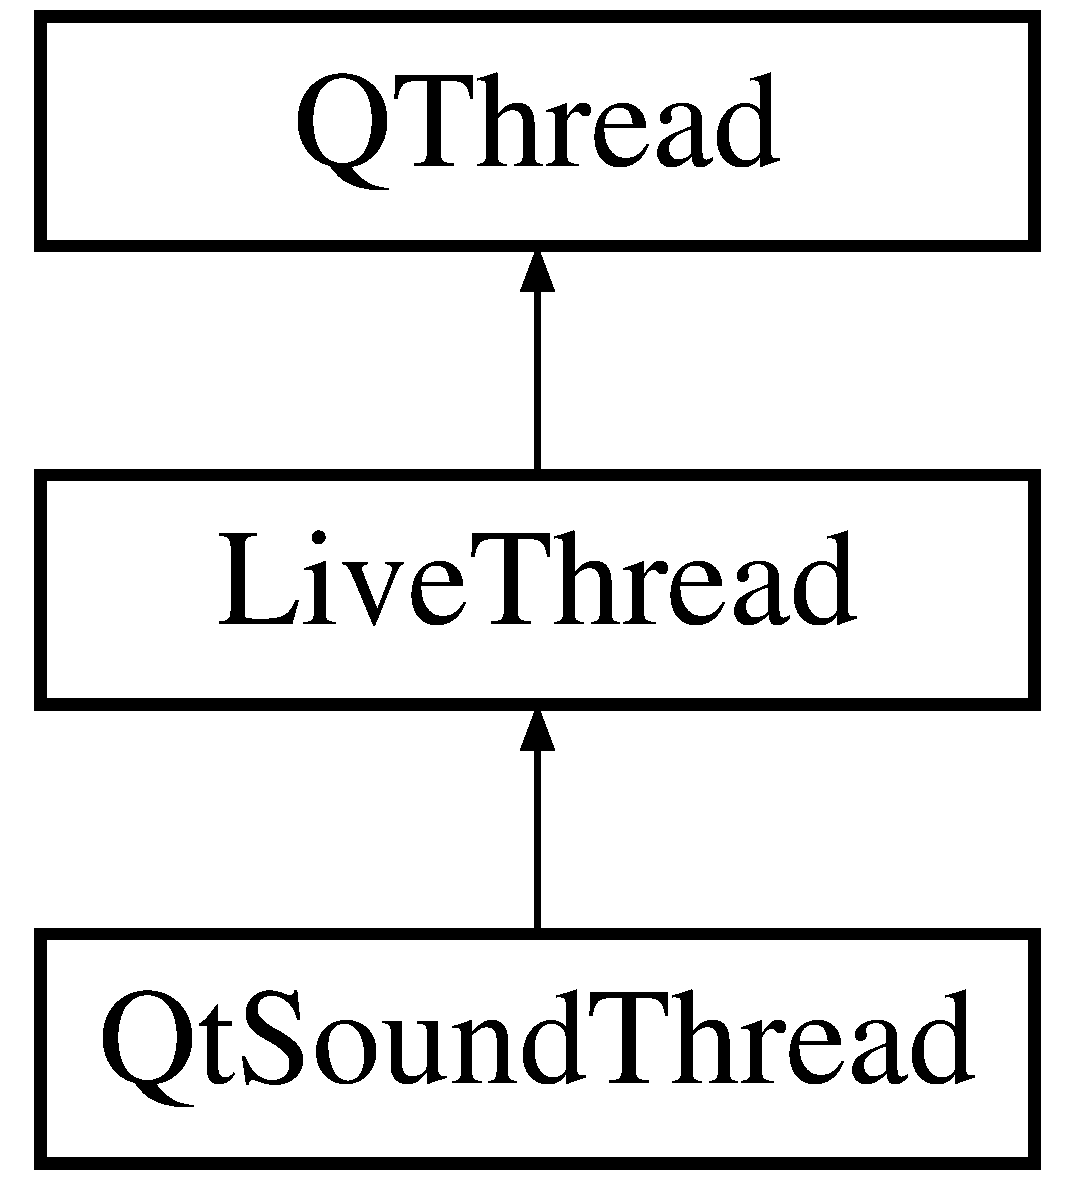
\includegraphics[height=3.000000cm]{classQtSoundThread}
\end{center}
\end{figure}
\subsection*{Public Slots}
\begin{DoxyCompactItemize}
\item 
\hypertarget{classQtSoundThread_a57899ed97f7d2d1d5dcc4fa49dd5ff7e}{void {\bfseries done\+Signal\+Received} (Q\+String exception)}\label{classQtSoundThread_a57899ed97f7d2d1d5dcc4fa49dd5ff7e}

\end{DoxyCompactItemize}
\subsection*{Signals}
\begin{DoxyCompactItemize}
\item 
\hypertarget{classQtSoundThread_af32283e8f2e3482e98796880715e779e}{void {\bfseries done\+Signal} (\hyperlink{classQtSoundThread}{Qt\+Sound\+Thread} $\ast$, Q\+String)}\label{classQtSoundThread_af32283e8f2e3482e98796880715e779e}

\end{DoxyCompactItemize}
\subsection*{Public Member Functions}
\begin{DoxyCompactItemize}
\item 
\hypertarget{classQtSoundThread_a2e0d96a054274862e8bb308042a2fc51}{{\bfseries Qt\+Sound\+Thread} (const long identity, Q\+Object $\ast$parent=0)}\label{classQtSoundThread_a2e0d96a054274862e8bb308042a2fc51}

\item 
\hypertarget{classQtSoundThread_a75d05a2b1b7229d30e259efc44ab591e}{void {\bfseries run} () Q\+\_\+\+D\+E\+C\+L\+\_\+\+O\+V\+E\+R\+R\+I\+D\+E}\label{classQtSoundThread_a75d05a2b1b7229d30e259efc44ab591e}

\item 
\hypertarget{classQtSoundThread_a1833428896d2db8c41410a7cb55b5246}{void {\bfseries initialize} (const Q\+String \&filename, const Q\+String \&instructions)}\label{classQtSoundThread_a1833428896d2db8c41410a7cb55b5246}

\item 
\hypertarget{classQtSoundThread_a3a682c0fe88abfa08d01e24951ce8089}{bool {\bfseries update\+Code} (const Q\+String \&filename, const Q\+String \&code)}\label{classQtSoundThread_a3a682c0fe88abfa08d01e24951ce8089}

\end{DoxyCompactItemize}
\subsection*{Public Attributes}
\begin{DoxyCompactItemize}
\item 
\hypertarget{classLiveThread_a5cfdefd7574fb1f34bbe1d21b5e3c1d8}{const long {\bfseries I\+D}}\label{classLiveThread_a5cfdefd7574fb1f34bbe1d21b5e3c1d8}

\end{DoxyCompactItemize}


The documentation for this class was generated from the following file\+:\begin{DoxyCompactItemize}
\item 
src/Live\+Thread.\+hpp\end{DoxyCompactItemize}

\hypertarget{classRenderer}{\section{Renderer Class Reference}
\label{classRenderer}\index{Renderer@{Renderer}}
}


The \hyperlink{classRenderer}{Renderer} class.  




{\ttfamily \#include $<$Renderer.\+hpp$>$}

Inheritance diagram for Renderer\+:\begin{figure}[H]
\begin{center}
\leavevmode
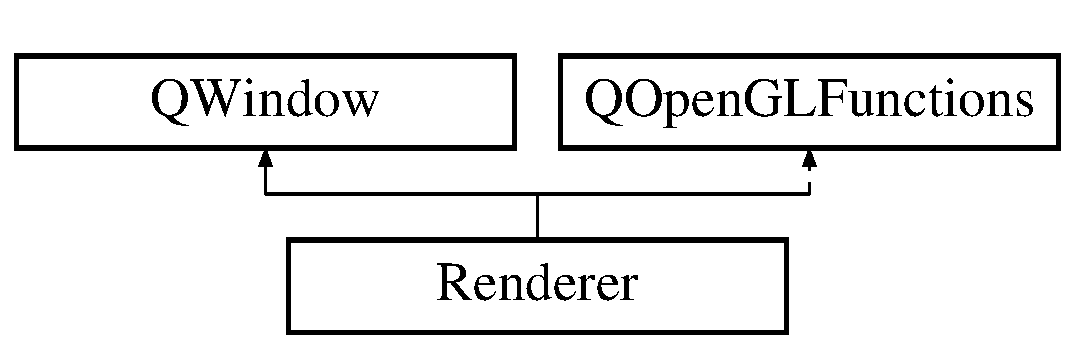
\includegraphics[height=2.000000cm]{classRenderer}
\end{center}
\end{figure}
\subsection*{Public Slots}
\begin{DoxyCompactItemize}
\item 
void \hyperlink{classRenderer_aff000964f75549d4f0089b0d7f914d4e}{render\+Now} ()
\begin{DoxyCompactList}\small\item\em \hyperlink{classRenderer_aff000964f75549d4f0089b0d7f914d4e}{Renderer\+::render\+Now}. \end{DoxyCompactList}\item 
void \hyperlink{classRenderer_a7a56362ec6a3e9e17f217668152a7252}{render\+Later} ()
\begin{DoxyCompactList}\small\item\em \hyperlink{classRenderer_a7a56362ec6a3e9e17f217668152a7252}{Renderer\+::render\+Later}. \end{DoxyCompactList}\item 
bool \hyperlink{classRenderer_ada11b323b6e47935245a4ffc3c2f34eb}{update\+Code} (const Q\+String \&, const Q\+String \&)
\begin{DoxyCompactList}\small\item\em \hyperlink{classRenderer_ada11b323b6e47935245a4ffc3c2f34eb}{Renderer\+::update\+Code}. \end{DoxyCompactList}\item 
void \hyperlink{classRenderer_a941e09f5b257fcf3a90e0a19b61096b4}{update\+Audio\+Data} (Q\+Byte\+Array)
\begin{DoxyCompactList}\small\item\em \hyperlink{classRenderer_a941e09f5b257fcf3a90e0a19b61096b4}{Renderer\+::update\+Audio\+Data}. \end{DoxyCompactList}\item 
void \hyperlink{classRenderer_acf65d29d7d1a3062a3d4bdb9e028fb23}{on\+Message\+Logged} (Q\+Open\+G\+L\+Debug\+Message message)
\begin{DoxyCompactList}\small\item\em \hyperlink{classRenderer_acf65d29d7d1a3062a3d4bdb9e028fb23}{Renderer\+::on\+Message\+Logged}. \end{DoxyCompactList}\end{DoxyCompactItemize}
\subsection*{Signals}
\begin{DoxyCompactItemize}
\item 
\hypertarget{classRenderer_a14700ec0055b02afe599c38fbb9fcaaf}{void {\bfseries done\+Signal} (Q\+String)}\label{classRenderer_a14700ec0055b02afe599c38fbb9fcaaf}

\item 
\hypertarget{classRenderer_a20f6d728a4c5edb06dcadef1b77e5ad4}{void {\bfseries errored} (Q\+String, int)}\label{classRenderer_a20f6d728a4c5edb06dcadef1b77e5ad4}

\end{DoxyCompactItemize}
\subsection*{Public Member Functions}
\begin{DoxyCompactItemize}
\item 
\hyperlink{classRenderer_a2d643cc466801828fb8ed0648ef72f4e}{Renderer} (Q\+Window $\ast$parent=0)
\begin{DoxyCompactList}\small\item\em \hyperlink{classRenderer_a2d643cc466801828fb8ed0648ef72f4e}{Renderer\+::\+Renderer}. \end{DoxyCompactList}\item 
\hyperlink{classRenderer_adbcd6b6f408774611cb936f9a781f00d}{Renderer} (const Q\+String \&, const Q\+String \&, Q\+Window $\ast$parent=0)
\begin{DoxyCompactList}\small\item\em \hyperlink{classRenderer_a2d643cc466801828fb8ed0648ef72f4e}{Renderer\+::\+Renderer}. \end{DoxyCompactList}\item 
\hyperlink{classRenderer_afeee408862d5bd6255a6882d47e6d5cd}{$\sim$\+Renderer} ()
\begin{DoxyCompactList}\small\item\em \hyperlink{classRenderer_afeee408862d5bd6255a6882d47e6d5cd}{Renderer\+::$\sim$\+Renderer}. \end{DoxyCompactList}\end{DoxyCompactItemize}
\subsection*{Protected Member Functions}
\begin{DoxyCompactItemize}
\item 
virtual bool \hyperlink{classRenderer_aa08452b84c6b687b62650322e8a05ec2}{event} (Q\+Event $\ast$)
\begin{DoxyCompactList}\small\item\em \hyperlink{classRenderer_aa08452b84c6b687b62650322e8a05ec2}{Renderer\+::event}. \end{DoxyCompactList}\item 
virtual void \hyperlink{classRenderer_a58526fa539582364b1e233d917a1d7f0}{expose\+Event} (Q\+Expose\+Event $\ast$)
\begin{DoxyCompactList}\small\item\em \hyperlink{classRenderer_a58526fa539582364b1e233d917a1d7f0}{Renderer\+::expose\+Event}. \end{DoxyCompactList}\end{DoxyCompactItemize}


\subsection{Detailed Description}
The \hyperlink{classRenderer}{Renderer} class. 

A subclass of Q\+Window and Q\+O\+Pen\+G\+L\+Functions that implements a G\+L\+S\+L fragment shader renderer. 

\subsection{Constructor \& Destructor Documentation}
\hypertarget{classRenderer_a2d643cc466801828fb8ed0648ef72f4e}{\index{Renderer@{Renderer}!Renderer@{Renderer}}
\index{Renderer@{Renderer}!Renderer@{Renderer}}
\subsubsection[{Renderer}]{\setlength{\rightskip}{0pt plus 5cm}Renderer\+::\+Renderer (
\begin{DoxyParamCaption}
\item[{Q\+Window $\ast$}]{parent = {\ttfamily 0}}
\end{DoxyParamCaption}
)\hspace{0.3cm}{\ttfamily [explicit]}}}\label{classRenderer_a2d643cc466801828fb8ed0648ef72f4e}


\hyperlink{classRenderer_a2d643cc466801828fb8ed0648ef72f4e}{Renderer\+::\+Renderer}. 


\begin{DoxyParams}{Parameters}
{\em parent} & Parent object of the render window\\
\hline
\end{DoxyParams}
Create a new \hyperlink{classRenderer}{Renderer} with default shader \hypertarget{classRenderer_adbcd6b6f408774611cb936f9a781f00d}{\index{Renderer@{Renderer}!Renderer@{Renderer}}
\index{Renderer@{Renderer}!Renderer@{Renderer}}
\subsubsection[{Renderer}]{\setlength{\rightskip}{0pt plus 5cm}Renderer\+::\+Renderer (
\begin{DoxyParamCaption}
\item[{const Q\+String \&}]{filename, }
\item[{const Q\+String \&}]{instructions, }
\item[{Q\+Window $\ast$}]{parent = {\ttfamily 0}}
\end{DoxyParamCaption}
)\hspace{0.3cm}{\ttfamily [explicit]}}}\label{classRenderer_adbcd6b6f408774611cb936f9a781f00d}


\hyperlink{classRenderer_a2d643cc466801828fb8ed0648ef72f4e}{Renderer\+::\+Renderer}. 


\begin{DoxyParams}{Parameters}
{\em filename} & Name that should shown in the title \\
\hline
{\em instructions} & Shader code for execution \\
\hline
{\em parent} & Parent object of the render window\\
\hline
\end{DoxyParams}
Create a new \hyperlink{classRenderer}{Renderer} with given code and set filename as title 

References on\+Message\+Logged(), and update\+Audio\+Data().

\hypertarget{classRenderer_afeee408862d5bd6255a6882d47e6d5cd}{\index{Renderer@{Renderer}!````~Renderer@{$\sim$\+Renderer}}
\index{````~Renderer@{$\sim$\+Renderer}!Renderer@{Renderer}}
\subsubsection[{$\sim$\+Renderer}]{\setlength{\rightskip}{0pt plus 5cm}Renderer\+::$\sim$\+Renderer (
\begin{DoxyParamCaption}
{}
\end{DoxyParamCaption}
)}}\label{classRenderer_afeee408862d5bd6255a6882d47e6d5cd}


\hyperlink{classRenderer_afeee408862d5bd6255a6882d47e6d5cd}{Renderer\+::$\sim$\+Renderer}. 

Free resources 

\subsection{Member Function Documentation}
\hypertarget{classRenderer_aa08452b84c6b687b62650322e8a05ec2}{\index{Renderer@{Renderer}!event@{event}}
\index{event@{event}!Renderer@{Renderer}}
\subsubsection[{event}]{\setlength{\rightskip}{0pt plus 5cm}bool Renderer\+::event (
\begin{DoxyParamCaption}
\item[{Q\+Event $\ast$}]{event}
\end{DoxyParamCaption}
)\hspace{0.3cm}{\ttfamily [protected]}, {\ttfamily [virtual]}}}\label{classRenderer_aa08452b84c6b687b62650322e8a05ec2}


\hyperlink{classRenderer_aa08452b84c6b687b62650322e8a05ec2}{Renderer\+::event}. 


\begin{DoxyParams}{Parameters}
{\em event} & The event that should be proccessed \\
\hline
\end{DoxyParams}
\begin{DoxyReturn}{Returns}
True if the event was successful proccessed, otherwise false
\end{DoxyReturn}
Called if a new event is poped from the event-\/queue to render on update event and Q\+\_\+\+E\+M\+I\+T done\+Signal on close event. 

References render\+Now().

\hypertarget{classRenderer_a58526fa539582364b1e233d917a1d7f0}{\index{Renderer@{Renderer}!expose\+Event@{expose\+Event}}
\index{expose\+Event@{expose\+Event}!Renderer@{Renderer}}
\subsubsection[{expose\+Event}]{\setlength{\rightskip}{0pt plus 5cm}void Renderer\+::expose\+Event (
\begin{DoxyParamCaption}
\item[{Q\+Expose\+Event $\ast$}]{}
\end{DoxyParamCaption}
)\hspace{0.3cm}{\ttfamily [protected]}, {\ttfamily [virtual]}}}\label{classRenderer_a58526fa539582364b1e233d917a1d7f0}


\hyperlink{classRenderer_a58526fa539582364b1e233d917a1d7f0}{Renderer\+::expose\+Event}. 

Called if the window is ready to start rendering 

References render\+Now().

\hypertarget{classRenderer_acf65d29d7d1a3062a3d4bdb9e028fb23}{\index{Renderer@{Renderer}!on\+Message\+Logged@{on\+Message\+Logged}}
\index{on\+Message\+Logged@{on\+Message\+Logged}!Renderer@{Renderer}}
\subsubsection[{on\+Message\+Logged}]{\setlength{\rightskip}{0pt plus 5cm}void Renderer\+::on\+Message\+Logged (
\begin{DoxyParamCaption}
\item[{Q\+Open\+G\+L\+Debug\+Message}]{message}
\end{DoxyParamCaption}
)\hspace{0.3cm}{\ttfamily [slot]}}}\label{classRenderer_acf65d29d7d1a3062a3d4bdb9e028fb23}


\hyperlink{classRenderer_acf65d29d7d1a3062a3d4bdb9e028fb23}{Renderer\+::on\+Message\+Logged}. 


\begin{DoxyParams}{Parameters}
{\em message} & Message text\\
\hline
\end{DoxyParams}
Write the message text in the debug output 

Referenced by Renderer().

\hypertarget{classRenderer_a7a56362ec6a3e9e17f217668152a7252}{\index{Renderer@{Renderer}!render\+Later@{render\+Later}}
\index{render\+Later@{render\+Later}!Renderer@{Renderer}}
\subsubsection[{render\+Later}]{\setlength{\rightskip}{0pt plus 5cm}void Renderer\+::render\+Later (
\begin{DoxyParamCaption}
{}
\end{DoxyParamCaption}
)\hspace{0.3cm}{\ttfamily [slot]}}}\label{classRenderer_a7a56362ec6a3e9e17f217668152a7252}


\hyperlink{classRenderer_a7a56362ec6a3e9e17f217668152a7252}{Renderer\+::render\+Later}. 

Enqueue an update event to event queue 

Referenced by render\+Now().

\hypertarget{classRenderer_aff000964f75549d4f0089b0d7f914d4e}{\index{Renderer@{Renderer}!render\+Now@{render\+Now}}
\index{render\+Now@{render\+Now}!Renderer@{Renderer}}
\subsubsection[{render\+Now}]{\setlength{\rightskip}{0pt plus 5cm}void Renderer\+::render\+Now (
\begin{DoxyParamCaption}
{}
\end{DoxyParamCaption}
)\hspace{0.3cm}{\ttfamily [slot]}}}\label{classRenderer_aff000964f75549d4f0089b0d7f914d4e}


\hyperlink{classRenderer_aff000964f75549d4f0089b0d7f914d4e}{Renderer\+::render\+Now}. 

Use the compiled shader to render on the widget 

References render\+Later().



Referenced by event(), and expose\+Event().

\hypertarget{classRenderer_a941e09f5b257fcf3a90e0a19b61096b4}{\index{Renderer@{Renderer}!update\+Audio\+Data@{update\+Audio\+Data}}
\index{update\+Audio\+Data@{update\+Audio\+Data}!Renderer@{Renderer}}
\subsubsection[{update\+Audio\+Data}]{\setlength{\rightskip}{0pt plus 5cm}void Renderer\+::update\+Audio\+Data (
\begin{DoxyParamCaption}
\item[{Q\+Byte\+Array}]{data}
\end{DoxyParamCaption}
)\hspace{0.3cm}{\ttfamily [slot]}}}\label{classRenderer_a941e09f5b257fcf3a90e0a19b61096b4}


\hyperlink{classRenderer_a941e09f5b257fcf3a90e0a19b61096b4}{Renderer\+::update\+Audio\+Data}. 


\begin{DoxyParams}{Parameters}
{\em data} & New audio data\\
\hline
\end{DoxyParams}
Copy the new sound-\/data to the graphics memory for visualisation 

Referenced by Renderer().

\hypertarget{classRenderer_ada11b323b6e47935245a4ffc3c2f34eb}{\index{Renderer@{Renderer}!update\+Code@{update\+Code}}
\index{update\+Code@{update\+Code}!Renderer@{Renderer}}
\subsubsection[{update\+Code}]{\setlength{\rightskip}{0pt plus 5cm}bool Renderer\+::update\+Code (
\begin{DoxyParamCaption}
\item[{const Q\+String \&}]{filename, }
\item[{const Q\+String \&}]{code}
\end{DoxyParamCaption}
)\hspace{0.3cm}{\ttfamily [slot]}}}\label{classRenderer_ada11b323b6e47935245a4ffc3c2f34eb}


\hyperlink{classRenderer_ada11b323b6e47935245a4ffc3c2f34eb}{Renderer\+::update\+Code}. 


\begin{DoxyParams}{Parameters}
{\em filename} & Text for the title \\
\hline
{\em code} & New shader program code \\
\hline
\end{DoxyParams}
\begin{DoxyReturn}{Returns}
True on success, otherwise false.
\end{DoxyReturn}
Set new title and compile new code for the shader program 

The documentation for this class was generated from the following files\+:\begin{DoxyCompactItemize}
\item 
src/Renderer.\+hpp\item 
src/Renderer.\+cpp\end{DoxyCompactItemize}

\hypertarget{classSettingsBackend}{\section{Settings\+Backend Class Reference}
\label{classSettingsBackend}\index{Settings\+Backend@{Settings\+Backend}}
}


The \hyperlink{classSettingsBackend}{Settings\+Backend} class.  




{\ttfamily \#include $<$Settings\+Backend.\+hpp$>$}

\subsection*{Static Public Member Functions}
\begin{DoxyCompactItemize}
\item 
static Q\+Variant \hyperlink{classSettingsBackend_aa88d1c980c78acfcb67fb3d76e8a9e0f}{get\+Settings\+For} (Q\+String, const Q\+Variant \&)
\begin{DoxyCompactList}\small\item\em \hyperlink{classSettingsBackend_aa88d1c980c78acfcb67fb3d76e8a9e0f}{Settings\+Backend\+::get\+Settings\+For}. \end{DoxyCompactList}\item 
static Q\+Variant \hyperlink{classSettingsBackend_a654a3528f4142036f90c87bdc6637ce5}{get\+Settings\+For} (const Q\+String, const Q\+Variant, const int)
\begin{DoxyCompactList}\small\item\em \hyperlink{classSettingsBackend_aa88d1c980c78acfcb67fb3d76e8a9e0f}{Settings\+Backend\+::get\+Settings\+For}. \end{DoxyCompactList}\item 
static Q\+Hash$<$ Q\+String, Q\+Variant $>$ \hyperlink{classSettingsBackend_a3dbcf97357969ab42f347d8e4e9a9ca4}{get\+Settings} (const int index)
\begin{DoxyCompactList}\small\item\em \hyperlink{classSettingsBackend_a3dbcf97357969ab42f347d8e4e9a9ca4}{Settings\+Backend\+::get\+Settings}. \end{DoxyCompactList}\item 
static void \hyperlink{classSettingsBackend_a674c2b36fbd38622c79c47b3bcb60e68}{add\+Settings} (const Q\+String key, const Q\+Variant value)
\begin{DoxyCompactList}\small\item\em \hyperlink{classSettingsBackend_a674c2b36fbd38622c79c47b3bcb60e68}{Settings\+Backend\+::add\+Settings}. \end{DoxyCompactList}\item 
static void \hyperlink{classSettingsBackend_abaf70fb3c8f7c5e88d5f21b480ceb51d}{save\+Settings\+For} (const int id, const Q\+String \&key, const Q\+Variant \&value)
\begin{DoxyCompactList}\small\item\em Settings\+Backend\+::save\+Settings. \end{DoxyCompactList}\item 
\hypertarget{classSettingsBackend_a9685ad12f32b9f2c14c73bdb47b2b250}{static void {\bfseries save\+Settings\+For} (const int id, const Q\+Hash$<$ Q\+String, Q\+Variant $>$ \&)}\label{classSettingsBackend_a9685ad12f32b9f2c14c73bdb47b2b250}

\item 
static void \hyperlink{classSettingsBackend_ad5a3439570c0a5ee26d8d838c61d3063}{remove\+Settings} (const int)
\begin{DoxyCompactList}\small\item\em \hyperlink{classSettingsBackend_ad5a3439570c0a5ee26d8d838c61d3063}{Settings\+Backend\+::remove\+Settings}. \end{DoxyCompactList}\end{DoxyCompactItemize}


\subsection{Detailed Description}
The \hyperlink{classSettingsBackend}{Settings\+Backend} class. 

A settings backend. Reads from and writes to the platform independent persistent settings. 

\subsection{Member Function Documentation}
\hypertarget{classSettingsBackend_a674c2b36fbd38622c79c47b3bcb60e68}{\index{Settings\+Backend@{Settings\+Backend}!add\+Settings@{add\+Settings}}
\index{add\+Settings@{add\+Settings}!Settings\+Backend@{Settings\+Backend}}
\subsubsection[{add\+Settings}]{\setlength{\rightskip}{0pt plus 5cm}void Settings\+Backend\+::add\+Settings (
\begin{DoxyParamCaption}
\item[{const Q\+String}]{key, }
\item[{const Q\+Variant}]{value}
\end{DoxyParamCaption}
)\hspace{0.3cm}{\ttfamily [static]}}}\label{classSettingsBackend_a674c2b36fbd38622c79c47b3bcb60e68}


\hyperlink{classSettingsBackend_a674c2b36fbd38622c79c47b3bcb60e68}{Settings\+Backend\+::add\+Settings}. 


\begin{DoxyParams}{Parameters}
{\em key} & \\
\hline
{\em value} & Adds an entry to the global settings. \\
\hline
\end{DoxyParams}
\hypertarget{classSettingsBackend_a3dbcf97357969ab42f347d8e4e9a9ca4}{\index{Settings\+Backend@{Settings\+Backend}!get\+Settings@{get\+Settings}}
\index{get\+Settings@{get\+Settings}!Settings\+Backend@{Settings\+Backend}}
\subsubsection[{get\+Settings}]{\setlength{\rightskip}{0pt plus 5cm}Q\+Hash$<$ Q\+String, Q\+Variant $>$ Settings\+Backend\+::get\+Settings (
\begin{DoxyParamCaption}
\item[{const int}]{id}
\end{DoxyParamCaption}
)\hspace{0.3cm}{\ttfamily [static]}}}\label{classSettingsBackend_a3dbcf97357969ab42f347d8e4e9a9ca4}


\hyperlink{classSettingsBackend_a3dbcf97357969ab42f347d8e4e9a9ca4}{Settings\+Backend\+::get\+Settings}. 


\begin{DoxyParams}{Parameters}
{\em id} & \\
\hline
\end{DoxyParams}
\begin{DoxyReturn}{Returns}
the settings as a Q\+Hash
\end{DoxyReturn}
gets the settings for a child window and translates it to a Q\+Hash that is returned. 

Referenced by Backend\+::get\+Settings(), Backend\+::instance\+Request\+Settings(), and Settings\+Window\+::\+Settings\+Window().

\hypertarget{classSettingsBackend_aa88d1c980c78acfcb67fb3d76e8a9e0f}{\index{Settings\+Backend@{Settings\+Backend}!get\+Settings\+For@{get\+Settings\+For}}
\index{get\+Settings\+For@{get\+Settings\+For}!Settings\+Backend@{Settings\+Backend}}
\subsubsection[{get\+Settings\+For}]{\setlength{\rightskip}{0pt plus 5cm}Q\+Variant Settings\+Backend\+::get\+Settings\+For (
\begin{DoxyParamCaption}
\item[{Q\+String}]{key, }
\item[{const Q\+Variant \&}]{default\+Option}
\end{DoxyParamCaption}
)\hspace{0.3cm}{\ttfamily [static]}}}\label{classSettingsBackend_aa88d1c980c78acfcb67fb3d76e8a9e0f}


\hyperlink{classSettingsBackend_aa88d1c980c78acfcb67fb3d76e8a9e0f}{Settings\+Backend\+::get\+Settings\+For}. 


\begin{DoxyParams}{Parameters}
{\em key} & \\
\hline
{\em default\+Option} & \\
\hline
\end{DoxyParams}
\begin{DoxyReturn}{Returns}
the settings requested
\end{DoxyReturn}
Takes a key and a default option. Gets the settings for the key or returns default\+Option. 

Referenced by Backend\+::\+Backend(), Backend\+::instance\+Request\+Setting(), Backend\+::instance\+Run\+Code(), and Backend\+::load\+Ids().

\hypertarget{classSettingsBackend_a654a3528f4142036f90c87bdc6637ce5}{\index{Settings\+Backend@{Settings\+Backend}!get\+Settings\+For@{get\+Settings\+For}}
\index{get\+Settings\+For@{get\+Settings\+For}!Settings\+Backend@{Settings\+Backend}}
\subsubsection[{get\+Settings\+For}]{\setlength{\rightskip}{0pt plus 5cm}Q\+Variant Settings\+Backend\+::get\+Settings\+For (
\begin{DoxyParamCaption}
\item[{const Q\+String}]{key, }
\item[{const Q\+Variant}]{default\+Option, }
\item[{const int}]{id}
\end{DoxyParamCaption}
)\hspace{0.3cm}{\ttfamily [static]}}}\label{classSettingsBackend_a654a3528f4142036f90c87bdc6637ce5}


\hyperlink{classSettingsBackend_aa88d1c980c78acfcb67fb3d76e8a9e0f}{Settings\+Backend\+::get\+Settings\+For}. 


\begin{DoxyParams}{Parameters}
{\em key} & \\
\hline
{\em default\+Option} & \\
\hline
{\em id} & \\
\hline
\end{DoxyParams}
\begin{DoxyReturn}{Returns}
the settings requested
\end{DoxyReturn}
Takes a key, a default option and the index of the requesting child window. Gets the settings for the key or returns default\+Option. \hypertarget{classSettingsBackend_ad5a3439570c0a5ee26d8d838c61d3063}{\index{Settings\+Backend@{Settings\+Backend}!remove\+Settings@{remove\+Settings}}
\index{remove\+Settings@{remove\+Settings}!Settings\+Backend@{Settings\+Backend}}
\subsubsection[{remove\+Settings}]{\setlength{\rightskip}{0pt plus 5cm}void Settings\+Backend\+::remove\+Settings (
\begin{DoxyParamCaption}
\item[{const int}]{id}
\end{DoxyParamCaption}
)\hspace{0.3cm}{\ttfamily [static]}}}\label{classSettingsBackend_ad5a3439570c0a5ee26d8d838c61d3063}


\hyperlink{classSettingsBackend_ad5a3439570c0a5ee26d8d838c61d3063}{Settings\+Backend\+::remove\+Settings}. 


\begin{DoxyParams}{Parameters}
{\em id} & Removes the settings of a child. \\
\hline
\end{DoxyParams}


Referenced by Backend\+::add\+Instance(), Backend\+::child\+Said\+Close\+All(), and Backend\+::remove\+Settings().

\hypertarget{classSettingsBackend_abaf70fb3c8f7c5e88d5f21b480ceb51d}{\index{Settings\+Backend@{Settings\+Backend}!save\+Settings\+For@{save\+Settings\+For}}
\index{save\+Settings\+For@{save\+Settings\+For}!Settings\+Backend@{Settings\+Backend}}
\subsubsection[{save\+Settings\+For}]{\setlength{\rightskip}{0pt plus 5cm}void Settings\+Backend\+::save\+Settings\+For (
\begin{DoxyParamCaption}
\item[{const int}]{id, }
\item[{const Q\+String \&}]{key, }
\item[{const Q\+Variant \&}]{value}
\end{DoxyParamCaption}
)\hspace{0.3cm}{\ttfamily [static]}}}\label{classSettingsBackend_abaf70fb3c8f7c5e88d5f21b480ceb51d}


Settings\+Backend\+::save\+Settings. 


\begin{DoxyParams}{Parameters}
{\em id} & \\
\hline
{\em key} & \\
\hline
{\em value} & Saves the settings of a instance. \\
\hline
\end{DoxyParams}


Referenced by Backend\+::instance\+Changed\+Setting(), and Backend\+::instance\+Changed\+Settings().



The documentation for this class was generated from the following files\+:\begin{DoxyCompactItemize}
\item 
src/Settings\+Backend.\+hpp\item 
src/Settings\+Backend.\+cpp\end{DoxyCompactItemize}

\hypertarget{classSettingsTab}{\section{Settings\+Tab Class Reference}
\label{classSettingsTab}\index{Settings\+Tab@{Settings\+Tab}}
}


The \hyperlink{classSettingsTab}{Settings\+Tab} class.  




{\ttfamily \#include $<$Settings\+Tab.\+hpp$>$}

Inheritance diagram for Settings\+Tab\+:\begin{figure}[H]
\begin{center}
\leavevmode
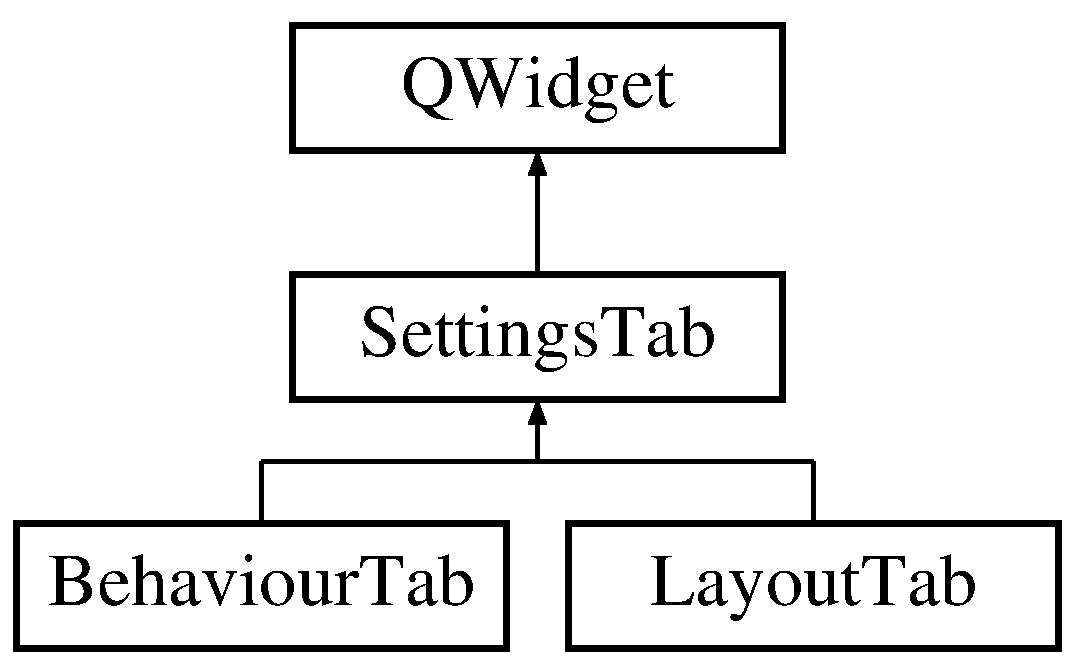
\includegraphics[height=3.000000cm]{classSettingsTab}
\end{center}
\end{figure}
\subsection*{Signals}
\begin{DoxyCompactItemize}
\item 
\hypertarget{classSettingsTab_ab72744b5433a111f3e79da0ef1d9af74}{void {\bfseries content\+Changed} ()}\label{classSettingsTab_ab72744b5433a111f3e79da0ef1d9af74}

\end{DoxyCompactItemize}
\subsection*{Public Member Functions}
\begin{DoxyCompactItemize}
\item 
\hyperlink{classSettingsTab_a8872d7984c5e66776e4d91db5ba761aa}{Settings\+Tab} (Q\+Hash$<$ Q\+String, Q\+Variant $>$ $\ast$Settings, Q\+Widget $\ast$parent=0)
\begin{DoxyCompactList}\small\item\em \hyperlink{classSettingsTab_a8872d7984c5e66776e4d91db5ba761aa}{Settings\+Tab\+::\+Settings\+Tab}. \end{DoxyCompactList}\end{DoxyCompactItemize}
\subsection*{Protected Attributes}
\begin{DoxyCompactItemize}
\item 
\hypertarget{classSettingsTab_af6d39f524ae1d31aa8655c1957939287}{Q\+Hash$<$ Q\+String, Q\+Variant $>$ $\ast$ {\bfseries settings}}\label{classSettingsTab_af6d39f524ae1d31aa8655c1957939287}

\end{DoxyCompactItemize}


\subsection{Detailed Description}
The \hyperlink{classSettingsTab}{Settings\+Tab} class. 

\begin{DoxyAuthor}{Author}
Veit Heller(s0539501) \& Tobias Brosge(s0539713)
\end{DoxyAuthor}
A subclass of Q\+Widget that implements a base class(not abstract) 

\subsection{Constructor \& Destructor Documentation}
\hypertarget{classSettingsTab_a8872d7984c5e66776e4d91db5ba761aa}{\index{Settings\+Tab@{Settings\+Tab}!Settings\+Tab@{Settings\+Tab}}
\index{Settings\+Tab@{Settings\+Tab}!Settings\+Tab@{Settings\+Tab}}
\subsubsection[{Settings\+Tab}]{\setlength{\rightskip}{0pt plus 5cm}Settings\+Tab\+::\+Settings\+Tab (
\begin{DoxyParamCaption}
\item[{Q\+Hash$<$ Q\+String, Q\+Variant $>$ $\ast$}]{Settings, }
\item[{Q\+Widget $\ast$}]{parent = {\ttfamily 0}}
\end{DoxyParamCaption}
)}}\label{classSettingsTab_a8872d7984c5e66776e4d91db5ba761aa}


\hyperlink{classSettingsTab_a8872d7984c5e66776e4d91db5ba761aa}{Settings\+Tab\+::\+Settings\+Tab}. 

The constructor of the \hyperlink{classSettingsTab}{Settings\+Tab} class. Translates the Q\+Settings into a list of strings and integers we can make use of. 

The documentation for this class was generated from the following files\+:\begin{DoxyCompactItemize}
\item 
src/Settings\+Tab.\+hpp\item 
src/Settings\+Tab.\+cpp\end{DoxyCompactItemize}

\hypertarget{classSettingsWindow}{\section{Settings\+Window Class Reference}
\label{classSettingsWindow}\index{Settings\+Window@{Settings\+Window}}
}


The \hyperlink{classSettingsWindow}{Settings\+Window} class.  




{\ttfamily \#include $<$Settings\+Window.\+hpp$>$}

Inheritance diagram for Settings\+Window\+:\begin{figure}[H]
\begin{center}
\leavevmode
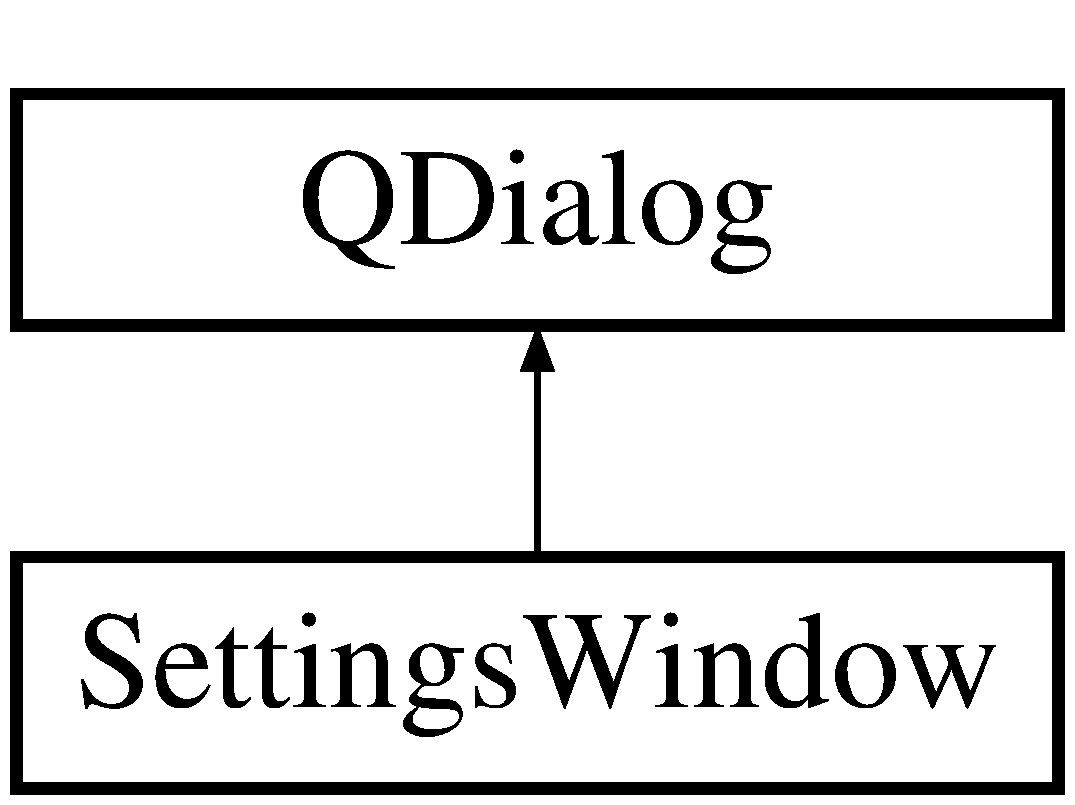
\includegraphics[height=2.000000cm]{classSettingsWindow}
\end{center}
\end{figure}
\subsection*{Public Member Functions}
\begin{DoxyCompactItemize}
\item 
\hyperlink{classSettingsWindow_aac6f02aa8c1e5022faacdf1c17c101d9}{Settings\+Window} (int)
\begin{DoxyCompactList}\small\item\em \hyperlink{classSettingsWindow_aac6f02aa8c1e5022faacdf1c17c101d9}{Settings\+Window\+::\+Settings\+Window}. \end{DoxyCompactList}\item 
\hyperlink{classSettingsWindow_a380a4a1227c28e0b3499175b10cea230}{$\sim$\+Settings\+Window} ()
\begin{DoxyCompactList}\small\item\em \hyperlink{classSettingsWindow_a380a4a1227c28e0b3499175b10cea230}{Settings\+Window\+::$\sim$\+Settings\+Window}. \end{DoxyCompactList}\end{DoxyCompactItemize}


\subsection{Detailed Description}
The \hyperlink{classSettingsWindow}{Settings\+Window} class. 

\begin{DoxyAuthor}{Author}
Veit Heller(s0539501) \& Tobias Brosge(s0539713)
\end{DoxyAuthor}
A subclass of Q\+Dialog that implements a Settings Window in which various configurations regarding behaviour and layout of the editor can be made. 

\subsection{Constructor \& Destructor Documentation}
\hypertarget{classSettingsWindow_aac6f02aa8c1e5022faacdf1c17c101d9}{\index{Settings\+Window@{Settings\+Window}!Settings\+Window@{Settings\+Window}}
\index{Settings\+Window@{Settings\+Window}!Settings\+Window@{Settings\+Window}}
\subsubsection[{Settings\+Window}]{\setlength{\rightskip}{0pt plus 5cm}Settings\+Window\+::\+Settings\+Window (
\begin{DoxyParamCaption}
\item[{int}]{sub\+Dir\+Num}
\end{DoxyParamCaption}
)}}\label{classSettingsWindow_aac6f02aa8c1e5022faacdf1c17c101d9}


\hyperlink{classSettingsWindow_aac6f02aa8c1e5022faacdf1c17c101d9}{Settings\+Window\+::\+Settings\+Window}. 

The constructor of the settings window. Sets up the S\+I\+G\+N\+A\+L\+S, U\+I and the tabs. 

References Settings\+Backend\+::get\+Settings().

\hypertarget{classSettingsWindow_a380a4a1227c28e0b3499175b10cea230}{\index{Settings\+Window@{Settings\+Window}!````~Settings\+Window@{$\sim$\+Settings\+Window}}
\index{````~Settings\+Window@{$\sim$\+Settings\+Window}!Settings\+Window@{Settings\+Window}}
\subsubsection[{$\sim$\+Settings\+Window}]{\setlength{\rightskip}{0pt plus 5cm}Settings\+Window\+::$\sim$\+Settings\+Window (
\begin{DoxyParamCaption}
{}
\end{DoxyParamCaption}
)}}\label{classSettingsWindow_a380a4a1227c28e0b3499175b10cea230}


\hyperlink{classSettingsWindow_a380a4a1227c28e0b3499175b10cea230}{Settings\+Window\+::$\sim$\+Settings\+Window}. 

Destructor of the \hyperlink{classSettingsWindow}{Settings\+Window} class. Cleans up after the window was close. 

The documentation for this class was generated from the following files\+:\begin{DoxyCompactItemize}
\item 
src/Settings\+Window.\+hpp\item 
src/Settings\+Window.\+cpp\end{DoxyCompactItemize}

\hypertarget{classSoundGenerator}{\section{Sound\+Generator Class Reference}
\label{classSoundGenerator}\index{Sound\+Generator@{Sound\+Generator}}
}


The \hyperlink{classSoundGenerator}{Sound\+Generator} class.  




{\ttfamily \#include $<$Sound\+Generator.\+hpp$>$}

Inheritance diagram for Sound\+Generator\+:\begin{figure}[H]
\begin{center}
\leavevmode
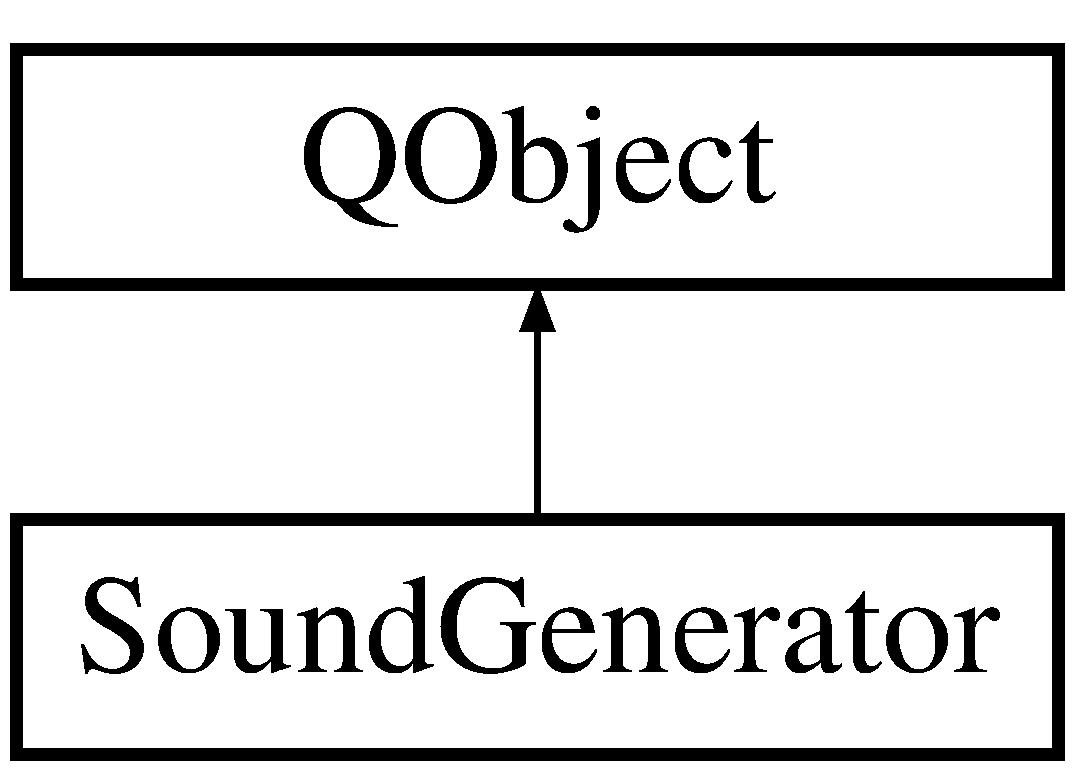
\includegraphics[height=2.000000cm]{classSoundGenerator}
\end{center}
\end{figure}
\subsection*{Signals}
\begin{DoxyCompactItemize}
\item 
\hypertarget{classSoundGenerator_a66f09f54619f0888b925f8181ab3c76a}{void {\bfseries done\+Signal} (Q\+String)}\label{classSoundGenerator_a66f09f54619f0888b925f8181ab3c76a}

\end{DoxyCompactItemize}
\subsection*{Public Member Functions}
\begin{DoxyCompactItemize}
\item 
\hyperlink{classSoundGenerator_a2b80d41c44e091422cdcb6b4e18a2f4e}{Sound\+Generator} (const Q\+String \&, const Q\+String \&)
\begin{DoxyCompactList}\small\item\em \hyperlink{classSoundGenerator_a2b80d41c44e091422cdcb6b4e18a2f4e}{Sound\+Generator\+::\+Sound\+Generator}. \end{DoxyCompactList}\item 
void \hyperlink{classSoundGenerator_acf7c58cd0d9ec25652bfbe9e2e27142f}{run} ()
\begin{DoxyCompactList}\small\item\em \hyperlink{classSoundGenerator_acf7c58cd0d9ec25652bfbe9e2e27142f}{Sound\+Generator\+::run}. \end{DoxyCompactList}\item 
bool \hyperlink{classSoundGenerator_a69366b95a600f0520603a9848c4fc17f}{update\+Code} (const Q\+String \&, const Q\+String \&)
\begin{DoxyCompactList}\small\item\em \hyperlink{classSoundGenerator_a69366b95a600f0520603a9848c4fc17f}{Sound\+Generator\+::update\+Code}. \end{DoxyCompactList}\end{DoxyCompactItemize}


\subsection{Detailed Description}
The \hyperlink{classSoundGenerator}{Sound\+Generator} class. 

\begin{DoxyAuthor}{Author}
Veit Heller(s0539501) \& Tobias Brosge(s0539713)
\end{DoxyAuthor}
A subclass of Q\+Thread that implements an environment for sound live coding while keeping the main codeeditor thread clean by dispatching. Q\+M\+L-\/based. 

\subsection{Constructor \& Destructor Documentation}
\hypertarget{classSoundGenerator_a2b80d41c44e091422cdcb6b4e18a2f4e}{\index{Sound\+Generator@{Sound\+Generator}!Sound\+Generator@{Sound\+Generator}}
\index{Sound\+Generator@{Sound\+Generator}!Sound\+Generator@{Sound\+Generator}}
\subsubsection[{Sound\+Generator}]{\setlength{\rightskip}{0pt plus 5cm}Sound\+Generator\+::\+Sound\+Generator (
\begin{DoxyParamCaption}
\item[{const Q\+String \&}]{prog\+Name, }
\item[{const Q\+String \&}]{qt\+Instructions}
\end{DoxyParamCaption}
)}}\label{classSoundGenerator_a2b80d41c44e091422cdcb6b4e18a2f4e}


\hyperlink{classSoundGenerator_a2b80d41c44e091422cdcb6b4e18a2f4e}{Sound\+Generator\+::\+Sound\+Generator}. 


\begin{DoxyParams}{Parameters}
{\em prog\+Name} & \\
\hline
{\em qt\+Instructions} & Constructor of the \hyperlink{classSoundGenerator}{Sound\+Generator} class. Sets up the Q\+M\+L interpreter, the class variables, the instructions and the break S\+I\+G\+N\+A\+L. \\
\hline
\end{DoxyParams}


\subsection{Member Function Documentation}
\hypertarget{classSoundGenerator_acf7c58cd0d9ec25652bfbe9e2e27142f}{\index{Sound\+Generator@{Sound\+Generator}!run@{run}}
\index{run@{run}!Sound\+Generator@{Sound\+Generator}}
\subsubsection[{run}]{\setlength{\rightskip}{0pt plus 5cm}void Sound\+Generator\+::run (
\begin{DoxyParamCaption}
{}
\end{DoxyParamCaption}
)}}\label{classSoundGenerator_acf7c58cd0d9ec25652bfbe9e2e27142f}


\hyperlink{classSoundGenerator_acf7c58cd0d9ec25652bfbe9e2e27142f}{Sound\+Generator\+::run}. 

the main loop of the thread, running until the user interrupts or the stopflag is set. \hypertarget{classSoundGenerator_a69366b95a600f0520603a9848c4fc17f}{\index{Sound\+Generator@{Sound\+Generator}!update\+Code@{update\+Code}}
\index{update\+Code@{update\+Code}!Sound\+Generator@{Sound\+Generator}}
\subsubsection[{update\+Code}]{\setlength{\rightskip}{0pt plus 5cm}bool Sound\+Generator\+::update\+Code (
\begin{DoxyParamCaption}
\item[{const Q\+String \&}]{filename, }
\item[{const Q\+String \&}]{qt\+Instructions}
\end{DoxyParamCaption}
)}}\label{classSoundGenerator_a69366b95a600f0520603a9848c4fc17f}


\hyperlink{classSoundGenerator_a69366b95a600f0520603a9848c4fc17f}{Sound\+Generator\+::update\+Code}. 


\begin{DoxyParams}{Parameters}
{\em filename} & \\
\hline
{\em qt\+Instructions} & \\
\hline
\end{DoxyParams}
\begin{DoxyReturn}{Returns}
true when name and instructions are valid, false otherwise 
\end{DoxyReturn}


The documentation for this class was generated from the following files\+:\begin{DoxyCompactItemize}
\item 
src/Sound\+Generator.\+hpp\item 
src/Sound\+Generator.\+cpp\end{DoxyCompactItemize}

\hypertarget{classInstances_1_1WindowInstance}{\section{Instances\+:\+:Window\+Instance Class Reference}
\label{classInstances_1_1WindowInstance}\index{Instances\+::\+Window\+Instance@{Instances\+::\+Window\+Instance}}
}


The Windownstance class.  




{\ttfamily \#include $<$Window\+Instance.\+hpp$>$}

Inheritance diagram for Instances\+:\+:Window\+Instance\+:\begin{figure}[H]
\begin{center}
\leavevmode
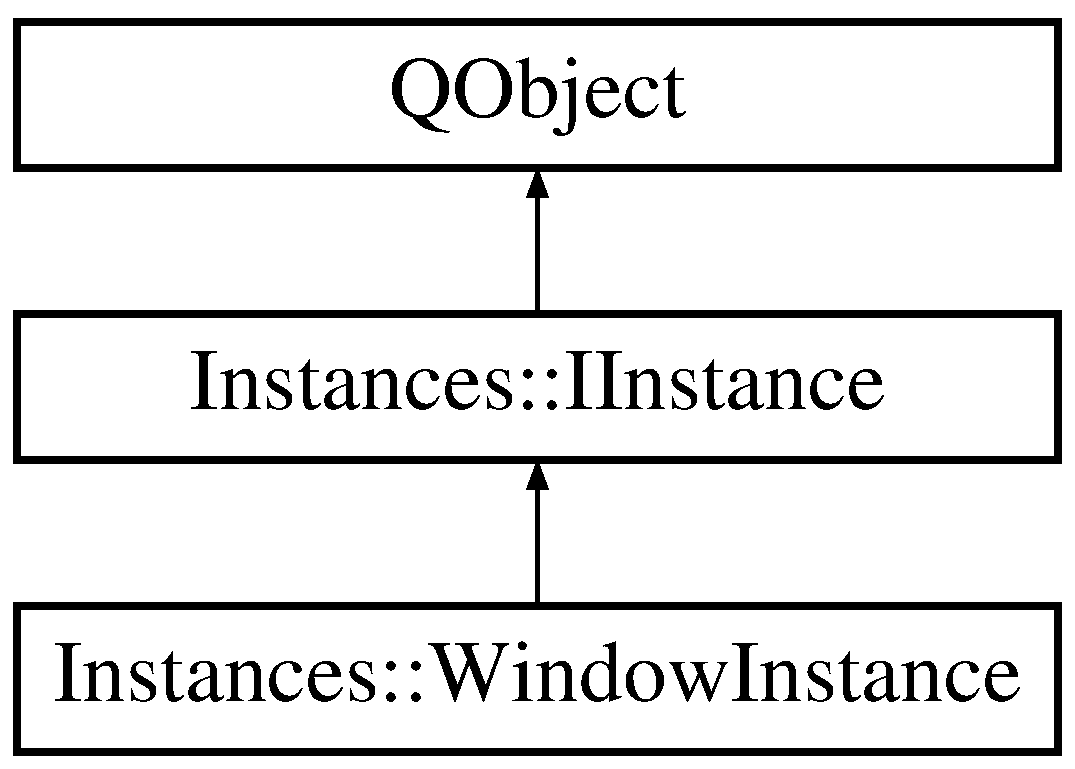
\includegraphics[height=3.000000cm]{classInstances_1_1WindowInstance}
\end{center}
\end{figure}
\subsection*{Public Slots}
\begin{DoxyCompactItemize}
\item 
\hypertarget{classInstances_1_1WindowInstance_a2d5c2c21c6b924bd2e88fafb474c7bd2}{void {\bfseries got\+Destroying} (Q\+Object $\ast$)}\label{classInstances_1_1WindowInstance_a2d5c2c21c6b924bd2e88fafb474c7bd2}

\item 
void \hyperlink{classInstances_1_1WindowInstance_ad6347ebd0f1af6c4b1ae1d843e97ce34}{got\+Closing} (\hyperlink{classEditorWindow}{Editor\+Window} $\ast$)
\begin{DoxyCompactList}\small\item\em \hyperlink{classInstances_1_1WindowInstance_ad6347ebd0f1af6c4b1ae1d843e97ce34}{Window\+Instance\+::got\+Closing}. \end{DoxyCompactList}\item 
void \hyperlink{classInstances_1_1WindowInstance_aed97db1c0bc35d41194c43eca97fa775}{got\+Close\+All} (\hyperlink{classEditorWindow}{Editor\+Window} $\ast$)
\begin{DoxyCompactList}\small\item\em \hyperlink{classInstances_1_1WindowInstance_aed97db1c0bc35d41194c43eca97fa775}{Window\+Instance\+::got\+Close\+All}. \end{DoxyCompactList}\item 
void \hyperlink{classInstances_1_1WindowInstance_ab9b5e2602b584217c2115fca0df87cb3}{got\+Run\+Code} (\hyperlink{classEditorWindow}{Editor\+Window} $\ast$)
\begin{DoxyCompactList}\small\item\em \hyperlink{classInstances_1_1WindowInstance_ab9b5e2602b584217c2115fca0df87cb3}{Window\+Instance\+::got\+Run\+Code}. \end{DoxyCompactList}\item 
void \hyperlink{classInstances_1_1WindowInstance_ab794a3a603f6b6ca75168383b9575524}{got\+Stop\+Code} (\hyperlink{classEditorWindow}{Editor\+Window} $\ast$)
\begin{DoxyCompactList}\small\item\em \hyperlink{classInstances_1_1WindowInstance_ab794a3a603f6b6ca75168383b9575524}{Window\+Instance\+::got\+Stop\+Code}. \end{DoxyCompactList}\item 
void \hyperlink{classInstances_1_1WindowInstance_ad1c5e3fc3c6f0675550786fb14f645a5}{got\+Open\+Help} (\hyperlink{classEditorWindow}{Editor\+Window} $\ast$)
\begin{DoxyCompactList}\small\item\em \hyperlink{classInstances_1_1WindowInstance_ad1c5e3fc3c6f0675550786fb14f645a5}{Window\+Instance\+::got\+Open\+Help}. \end{DoxyCompactList}\item 
void \hyperlink{classInstances_1_1WindowInstance_a166bf08fb12fe133212bea23d8564a24}{got\+Open\+Settings} (\hyperlink{classEditorWindow}{Editor\+Window} $\ast$)
\begin{DoxyCompactList}\small\item\em \hyperlink{classInstances_1_1WindowInstance_a166bf08fb12fe133212bea23d8564a24}{Window\+Instance\+::got\+Open\+Settings}. \end{DoxyCompactList}\item 
void \hyperlink{classInstances_1_1WindowInstance_afe1550c9ad22f89ef9b9b0f2163fd4e3}{got\+Changed\+Setting} (\hyperlink{classEditorWindow}{Editor\+Window} $\ast$, const Q\+String \&, const Q\+Variant \&)
\begin{DoxyCompactList}\small\item\em \hyperlink{classInstances_1_1WindowInstance_afe1550c9ad22f89ef9b9b0f2163fd4e3}{Window\+Instance\+::got\+Changed\+Setting}. \end{DoxyCompactList}\item 
void \hyperlink{classInstances_1_1WindowInstance_acfa637305b9db11854e230a58e8d4fde}{got\+Changed\+Settings} (\hyperlink{classEditorWindow}{Editor\+Window} $\ast$, const Q\+Hash$<$ Q\+String, Q\+Variant $>$ \&)
\begin{DoxyCompactList}\small\item\em \hyperlink{classInstances_1_1WindowInstance_acfa637305b9db11854e230a58e8d4fde}{Window\+Instance\+::got\+Changed\+Settings}. \end{DoxyCompactList}\end{DoxyCompactItemize}
\subsection*{Signals}
\begin{DoxyCompactItemize}
\item 
\hypertarget{classInstances_1_1IInstance_aa1981041a376e4c14ebca95df76cb041}{void {\bfseries run\+Code} (\hyperlink{classInstances_1_1IInstance}{I\+Instance} $\ast$)}\label{classInstances_1_1IInstance_aa1981041a376e4c14ebca95df76cb041}

\item 
\hypertarget{classInstances_1_1IInstance_aa2de904201702d2da2fd8fe9776fcfa5}{void {\bfseries stop\+Code} (\hyperlink{classInstances_1_1IInstance}{I\+Instance} $\ast$)}\label{classInstances_1_1IInstance_aa2de904201702d2da2fd8fe9776fcfa5}

\item 
\hypertarget{classInstances_1_1IInstance_acf3c3769af5448b3093e42b73e01c7e6}{void {\bfseries closing} (\hyperlink{classInstances_1_1IInstance}{I\+Instance} $\ast$)}\label{classInstances_1_1IInstance_acf3c3769af5448b3093e42b73e01c7e6}

\item 
\hypertarget{classInstances_1_1IInstance_a6f3b9855e287de954554c631bd7c0a8b}{void {\bfseries close\+All} ()}\label{classInstances_1_1IInstance_a6f3b9855e287de954554c631bd7c0a8b}

\item 
\hypertarget{classInstances_1_1IInstance_aea2d89deb68d4ba6d5833e03ff6a48dc}{void {\bfseries open\+Help} (\hyperlink{classInstances_1_1IInstance}{I\+Instance} $\ast$)}\label{classInstances_1_1IInstance_aea2d89deb68d4ba6d5833e03ff6a48dc}

\item 
\hypertarget{classInstances_1_1IInstance_a1864f99f3c54f539980c3e1a2ab2164d}{void {\bfseries open\+Settings} (\hyperlink{classInstances_1_1IInstance}{I\+Instance} $\ast$)}\label{classInstances_1_1IInstance_a1864f99f3c54f539980c3e1a2ab2164d}

\item 
\hypertarget{classInstances_1_1IInstance_a9ecdadd405b81e04a2b052b30efd6b9f}{void {\bfseries change\+Setting} (\hyperlink{classInstances_1_1IInstance}{I\+Instance} $\ast$, const Q\+String \&key, Q\+Variant value)}\label{classInstances_1_1IInstance_a9ecdadd405b81e04a2b052b30efd6b9f}

\item 
\hypertarget{classInstances_1_1IInstance_a4efdf11046ad14aaa6422dfe6eca761d}{void {\bfseries change\+Settings} (\hyperlink{classInstances_1_1IInstance}{I\+Instance} $\ast$, const Q\+Hash$<$ Q\+String, Q\+Variant $>$ \&)}\label{classInstances_1_1IInstance_a4efdf11046ad14aaa6422dfe6eca761d}

\item 
\hypertarget{classInstances_1_1IInstance_ab5dc40987e611bdc3036d59cf077d0e6}{void {\bfseries get\+Setting} (\hyperlink{classInstances_1_1IInstance}{I\+Instance} $\ast$, const Q\+String \&key, Q\+Variant \&value)}\label{classInstances_1_1IInstance_ab5dc40987e611bdc3036d59cf077d0e6}

\item 
\hypertarget{classInstances_1_1IInstance_a71691d22518c4f60f557c39c44de35b8}{void {\bfseries get\+Settings} (\hyperlink{classInstances_1_1IInstance}{I\+Instance} $\ast$, Q\+Hash$<$ Q\+String, Q\+Variant $>$ \&settings)}\label{classInstances_1_1IInstance_a71691d22518c4f60f557c39c44de35b8}

\end{DoxyCompactItemize}
\subsection*{Public Member Functions}
\begin{DoxyCompactItemize}
\item 
\hyperlink{classInstances_1_1WindowInstance_a93bf0b9976d49cb7a82d56e9ccb2d3cc}{Window\+Instance} (int id, const Q\+Hash$<$ Q\+String, Q\+Variant $>$ \&settings, Q\+Object $\ast$parent=0)
\begin{DoxyCompactList}\small\item\em \hyperlink{classInstances_1_1WindowInstance_a93bf0b9976d49cb7a82d56e9ccb2d3cc}{Window\+Instance\+::\+Window\+Instance}. \end{DoxyCompactList}\item 
\hyperlink{classInstances_1_1WindowInstance_abf76b416a3a63483a9daaf629726d7d5}{$\sim$\+Window\+Instance} ()
\begin{DoxyCompactList}\small\item\em \hyperlink{classInstances_1_1WindowInstance_abf76b416a3a63483a9daaf629726d7d5}{Window\+Instance\+::$\sim$\+Window\+Instance}. \end{DoxyCompactList}\item 
virtual Q\+String \hyperlink{classInstances_1_1WindowInstance_a9530a0b4cb1291a51bca31c7b7328f24}{source\+Code} () const 
\begin{DoxyCompactList}\small\item\em \hyperlink{classInstances_1_1WindowInstance_a9530a0b4cb1291a51bca31c7b7328f24}{Window\+Instance\+::source\+Code}. \end{DoxyCompactList}\item 
virtual Q\+String \hyperlink{classInstances_1_1WindowInstance_aae1b23157f3d6743f6db45a62bd5d5b4}{title} () const 
\begin{DoxyCompactList}\small\item\em \hyperlink{classInstances_1_1WindowInstance_aae1b23157f3d6743f6db45a62bd5d5b4}{Window\+Instance\+::title}. \end{DoxyCompactList}\item 
virtual bool \hyperlink{classInstances_1_1WindowInstance_a08129e171cbe49e26bc9d8d638502103}{close} ()
\begin{DoxyCompactList}\small\item\em \hyperlink{classInstances_1_1WindowInstance_a08129e171cbe49e26bc9d8d638502103}{Window\+Instance\+::close}. \end{DoxyCompactList}\item 
virtual void \hyperlink{classInstances_1_1WindowInstance_abf3cc6d6a38a682c1bd87f58806915dd}{report\+Error} (const Q\+String \&message)
\begin{DoxyCompactList}\small\item\em \hyperlink{classInstances_1_1WindowInstance_abf3cc6d6a38a682c1bd87f58806915dd}{Window\+Instance\+::report\+Error}. \end{DoxyCompactList}\item 
virtual void \hyperlink{classInstances_1_1WindowInstance_a92a296bb3476b0e8abe371d51b2e8dde}{report\+Warning} (const Q\+String \&)
\begin{DoxyCompactList}\small\item\em \hyperlink{classInstances_1_1WindowInstance_a92a296bb3476b0e8abe371d51b2e8dde}{Window\+Instance\+::report\+Warning}. \end{DoxyCompactList}\item 
virtual void \hyperlink{classInstances_1_1WindowInstance_a2fd33b23af086fddd16b6718d08f73d5}{highlight\+Errored\+Line} (int)
\begin{DoxyCompactList}\small\item\em \hyperlink{classInstances_1_1WindowInstance_a2fd33b23af086fddd16b6718d08f73d5}{Window\+Instance\+::highlight\+Errored\+Line}. \end{DoxyCompactList}\item 
virtual void \hyperlink{classInstances_1_1WindowInstance_a432a78ddfc8fdd62ae0d8e715bc57841}{code\+Stopped} ()
\begin{DoxyCompactList}\small\item\em \hyperlink{classInstances_1_1WindowInstance_a432a78ddfc8fdd62ae0d8e715bc57841}{Window\+Instance\+::code\+Stopped}. \end{DoxyCompactList}\end{DoxyCompactItemize}
\subsection*{Public Attributes}
\begin{DoxyCompactItemize}
\item 
\hypertarget{classInstances_1_1IInstance_a215b003cb2f0986801fa911533794b14}{const int {\bfseries I\+D}}\label{classInstances_1_1IInstance_a215b003cb2f0986801fa911533794b14}

\end{DoxyCompactItemize}


\subsection{Detailed Description}
The Windownstance class. 

Delegate from which all windows are derived that are managed by the backend. 

\subsection{Constructor \& Destructor Documentation}
\hypertarget{classInstances_1_1WindowInstance_a93bf0b9976d49cb7a82d56e9ccb2d3cc}{\index{Instances\+::\+Window\+Instance@{Instances\+::\+Window\+Instance}!Window\+Instance@{Window\+Instance}}
\index{Window\+Instance@{Window\+Instance}!Instances\+::\+Window\+Instance@{Instances\+::\+Window\+Instance}}
\subsubsection[{Window\+Instance}]{\setlength{\rightskip}{0pt plus 5cm}Instances\+::\+Window\+Instance\+::\+Window\+Instance (
\begin{DoxyParamCaption}
\item[{int}]{id, }
\item[{const Q\+Hash$<$ Q\+String, Q\+Variant $>$ \&}]{settings, }
\item[{Q\+Object $\ast$}]{parent = {\ttfamily 0}}
\end{DoxyParamCaption}
)}}\label{classInstances_1_1WindowInstance_a93bf0b9976d49cb7a82d56e9ccb2d3cc}


\hyperlink{classInstances_1_1WindowInstance_a93bf0b9976d49cb7a82d56e9ccb2d3cc}{Window\+Instance\+::\+Window\+Instance}. 


\begin{DoxyParams}{Parameters}
{\em id} & \\
\hline
{\em settings} & \\
\hline
{\em parent} & Constructor of the delegate. \\
\hline
\end{DoxyParams}
\hypertarget{classInstances_1_1WindowInstance_abf76b416a3a63483a9daaf629726d7d5}{\index{Instances\+::\+Window\+Instance@{Instances\+::\+Window\+Instance}!````~Window\+Instance@{$\sim$\+Window\+Instance}}
\index{````~Window\+Instance@{$\sim$\+Window\+Instance}!Instances\+::\+Window\+Instance@{Instances\+::\+Window\+Instance}}
\subsubsection[{$\sim$\+Window\+Instance}]{\setlength{\rightskip}{0pt plus 5cm}Instances\+::\+Window\+Instance\+::$\sim$\+Window\+Instance (
\begin{DoxyParamCaption}
{}
\end{DoxyParamCaption}
)}}\label{classInstances_1_1WindowInstance_abf76b416a3a63483a9daaf629726d7d5}


\hyperlink{classInstances_1_1WindowInstance_abf76b416a3a63483a9daaf629726d7d5}{Window\+Instance\+::$\sim$\+Window\+Instance}. 

Destructor of the delegate. 

\subsection{Member Function Documentation}
\hypertarget{classInstances_1_1WindowInstance_a08129e171cbe49e26bc9d8d638502103}{\index{Instances\+::\+Window\+Instance@{Instances\+::\+Window\+Instance}!close@{close}}
\index{close@{close}!Instances\+::\+Window\+Instance@{Instances\+::\+Window\+Instance}}
\subsubsection[{close}]{\setlength{\rightskip}{0pt plus 5cm}bool Instances\+::\+Window\+Instance\+::close (
\begin{DoxyParamCaption}
{}
\end{DoxyParamCaption}
)\hspace{0.3cm}{\ttfamily [virtual]}}}\label{classInstances_1_1WindowInstance_a08129e171cbe49e26bc9d8d638502103}


\hyperlink{classInstances_1_1WindowInstance_a08129e171cbe49e26bc9d8d638502103}{Window\+Instance\+::close}. 

\begin{DoxyReturn}{Returns}
whether closing has succeeded
\end{DoxyReturn}
Closes the editor window and return a success flag. 

Implements \hyperlink{classInstances_1_1IInstance}{Instances\+::\+I\+Instance}.



References got\+Closing().

\hypertarget{classInstances_1_1WindowInstance_a432a78ddfc8fdd62ae0d8e715bc57841}{\index{Instances\+::\+Window\+Instance@{Instances\+::\+Window\+Instance}!code\+Stopped@{code\+Stopped}}
\index{code\+Stopped@{code\+Stopped}!Instances\+::\+Window\+Instance@{Instances\+::\+Window\+Instance}}
\subsubsection[{code\+Stopped}]{\setlength{\rightskip}{0pt plus 5cm}void Instances\+::\+Window\+Instance\+::code\+Stopped (
\begin{DoxyParamCaption}
{}
\end{DoxyParamCaption}
)\hspace{0.3cm}{\ttfamily [virtual]}}}\label{classInstances_1_1WindowInstance_a432a78ddfc8fdd62ae0d8e715bc57841}


\hyperlink{classInstances_1_1WindowInstance_a432a78ddfc8fdd62ae0d8e715bc57841}{Window\+Instance\+::code\+Stopped}. 

Signals that execution of the editor code has finsihed. 

Implements \hyperlink{classInstances_1_1IInstance}{Instances\+::\+I\+Instance}.



References Editor\+Window\+::code\+Stopped().

\hypertarget{classInstances_1_1WindowInstance_afe1550c9ad22f89ef9b9b0f2163fd4e3}{\index{Instances\+::\+Window\+Instance@{Instances\+::\+Window\+Instance}!got\+Changed\+Setting@{got\+Changed\+Setting}}
\index{got\+Changed\+Setting@{got\+Changed\+Setting}!Instances\+::\+Window\+Instance@{Instances\+::\+Window\+Instance}}
\subsubsection[{got\+Changed\+Setting}]{\setlength{\rightskip}{0pt plus 5cm}void Instances\+::\+Window\+Instance\+::got\+Changed\+Setting (
\begin{DoxyParamCaption}
\item[{{\bf Editor\+Window} $\ast$}]{, }
\item[{const Q\+String \&}]{key, }
\item[{const Q\+Variant \&}]{value}
\end{DoxyParamCaption}
)\hspace{0.3cm}{\ttfamily [slot]}}}\label{classInstances_1_1WindowInstance_afe1550c9ad22f89ef9b9b0f2163fd4e3}


\hyperlink{classInstances_1_1WindowInstance_afe1550c9ad22f89ef9b9b0f2163fd4e3}{Window\+Instance\+::got\+Changed\+Setting}. 


\begin{DoxyParams}{Parameters}
{\em key} & \\
\hline
{\em value} & Signals that the editors' settings have changed(singla value). \\
\hline
\end{DoxyParams}
\hypertarget{classInstances_1_1WindowInstance_acfa637305b9db11854e230a58e8d4fde}{\index{Instances\+::\+Window\+Instance@{Instances\+::\+Window\+Instance}!got\+Changed\+Settings@{got\+Changed\+Settings}}
\index{got\+Changed\+Settings@{got\+Changed\+Settings}!Instances\+::\+Window\+Instance@{Instances\+::\+Window\+Instance}}
\subsubsection[{got\+Changed\+Settings}]{\setlength{\rightskip}{0pt plus 5cm}void Instances\+::\+Window\+Instance\+::got\+Changed\+Settings (
\begin{DoxyParamCaption}
\item[{{\bf Editor\+Window} $\ast$}]{, }
\item[{const Q\+Hash$<$ Q\+String, Q\+Variant $>$ \&}]{settings}
\end{DoxyParamCaption}
)\hspace{0.3cm}{\ttfamily [slot]}}}\label{classInstances_1_1WindowInstance_acfa637305b9db11854e230a58e8d4fde}


\hyperlink{classInstances_1_1WindowInstance_acfa637305b9db11854e230a58e8d4fde}{Window\+Instance\+::got\+Changed\+Settings}. 


\begin{DoxyParams}{Parameters}
{\em settings} & Signals that the editors' settings have changed(completely). \\
\hline
\end{DoxyParams}
\hypertarget{classInstances_1_1WindowInstance_aed97db1c0bc35d41194c43eca97fa775}{\index{Instances\+::\+Window\+Instance@{Instances\+::\+Window\+Instance}!got\+Close\+All@{got\+Close\+All}}
\index{got\+Close\+All@{got\+Close\+All}!Instances\+::\+Window\+Instance@{Instances\+::\+Window\+Instance}}
\subsubsection[{got\+Close\+All}]{\setlength{\rightskip}{0pt plus 5cm}void Instances\+::\+Window\+Instance\+::got\+Close\+All (
\begin{DoxyParamCaption}
\item[{{\bf Editor\+Window} $\ast$}]{}
\end{DoxyParamCaption}
)\hspace{0.3cm}{\ttfamily [slot]}}}\label{classInstances_1_1WindowInstance_aed97db1c0bc35d41194c43eca97fa775}


\hyperlink{classInstances_1_1WindowInstance_aed97db1c0bc35d41194c43eca97fa775}{Window\+Instance\+::got\+Close\+All}. 

Signals that the editor requested closing of all windows. \hypertarget{classInstances_1_1WindowInstance_ad6347ebd0f1af6c4b1ae1d843e97ce34}{\index{Instances\+::\+Window\+Instance@{Instances\+::\+Window\+Instance}!got\+Closing@{got\+Closing}}
\index{got\+Closing@{got\+Closing}!Instances\+::\+Window\+Instance@{Instances\+::\+Window\+Instance}}
\subsubsection[{got\+Closing}]{\setlength{\rightskip}{0pt plus 5cm}void Instances\+::\+Window\+Instance\+::got\+Closing (
\begin{DoxyParamCaption}
\item[{{\bf Editor\+Window} $\ast$}]{}
\end{DoxyParamCaption}
)\hspace{0.3cm}{\ttfamily [slot]}}}\label{classInstances_1_1WindowInstance_ad6347ebd0f1af6c4b1ae1d843e97ce34}


\hyperlink{classInstances_1_1WindowInstance_ad6347ebd0f1af6c4b1ae1d843e97ce34}{Window\+Instance\+::got\+Closing}. 

Signals that the editor requested closing. 

Referenced by close().

\hypertarget{classInstances_1_1WindowInstance_ad1c5e3fc3c6f0675550786fb14f645a5}{\index{Instances\+::\+Window\+Instance@{Instances\+::\+Window\+Instance}!got\+Open\+Help@{got\+Open\+Help}}
\index{got\+Open\+Help@{got\+Open\+Help}!Instances\+::\+Window\+Instance@{Instances\+::\+Window\+Instance}}
\subsubsection[{got\+Open\+Help}]{\setlength{\rightskip}{0pt plus 5cm}void Instances\+::\+Window\+Instance\+::got\+Open\+Help (
\begin{DoxyParamCaption}
\item[{{\bf Editor\+Window} $\ast$}]{}
\end{DoxyParamCaption}
)\hspace{0.3cm}{\ttfamily [slot]}}}\label{classInstances_1_1WindowInstance_ad1c5e3fc3c6f0675550786fb14f645a5}


\hyperlink{classInstances_1_1WindowInstance_ad1c5e3fc3c6f0675550786fb14f645a5}{Window\+Instance\+::got\+Open\+Help}. 

Signals that the editor requested a help window. \hypertarget{classInstances_1_1WindowInstance_a166bf08fb12fe133212bea23d8564a24}{\index{Instances\+::\+Window\+Instance@{Instances\+::\+Window\+Instance}!got\+Open\+Settings@{got\+Open\+Settings}}
\index{got\+Open\+Settings@{got\+Open\+Settings}!Instances\+::\+Window\+Instance@{Instances\+::\+Window\+Instance}}
\subsubsection[{got\+Open\+Settings}]{\setlength{\rightskip}{0pt plus 5cm}void Instances\+::\+Window\+Instance\+::got\+Open\+Settings (
\begin{DoxyParamCaption}
\item[{{\bf Editor\+Window} $\ast$}]{}
\end{DoxyParamCaption}
)\hspace{0.3cm}{\ttfamily [slot]}}}\label{classInstances_1_1WindowInstance_a166bf08fb12fe133212bea23d8564a24}


\hyperlink{classInstances_1_1WindowInstance_a166bf08fb12fe133212bea23d8564a24}{Window\+Instance\+::got\+Open\+Settings}. 

Signals that the editor requested a settings window. \hypertarget{classInstances_1_1WindowInstance_ab9b5e2602b584217c2115fca0df87cb3}{\index{Instances\+::\+Window\+Instance@{Instances\+::\+Window\+Instance}!got\+Run\+Code@{got\+Run\+Code}}
\index{got\+Run\+Code@{got\+Run\+Code}!Instances\+::\+Window\+Instance@{Instances\+::\+Window\+Instance}}
\subsubsection[{got\+Run\+Code}]{\setlength{\rightskip}{0pt plus 5cm}void Instances\+::\+Window\+Instance\+::got\+Run\+Code (
\begin{DoxyParamCaption}
\item[{{\bf Editor\+Window} $\ast$}]{}
\end{DoxyParamCaption}
)\hspace{0.3cm}{\ttfamily [slot]}}}\label{classInstances_1_1WindowInstance_ab9b5e2602b584217c2115fca0df87cb3}


\hyperlink{classInstances_1_1WindowInstance_ab9b5e2602b584217c2115fca0df87cb3}{Window\+Instance\+::got\+Run\+Code}. 

Signals that the editor requested a run. \hypertarget{classInstances_1_1WindowInstance_ab794a3a603f6b6ca75168383b9575524}{\index{Instances\+::\+Window\+Instance@{Instances\+::\+Window\+Instance}!got\+Stop\+Code@{got\+Stop\+Code}}
\index{got\+Stop\+Code@{got\+Stop\+Code}!Instances\+::\+Window\+Instance@{Instances\+::\+Window\+Instance}}
\subsubsection[{got\+Stop\+Code}]{\setlength{\rightskip}{0pt plus 5cm}void Instances\+::\+Window\+Instance\+::got\+Stop\+Code (
\begin{DoxyParamCaption}
\item[{{\bf Editor\+Window} $\ast$}]{}
\end{DoxyParamCaption}
)\hspace{0.3cm}{\ttfamily [slot]}}}\label{classInstances_1_1WindowInstance_ab794a3a603f6b6ca75168383b9575524}


\hyperlink{classInstances_1_1WindowInstance_ab794a3a603f6b6ca75168383b9575524}{Window\+Instance\+::got\+Stop\+Code}. 

Signals that the editor requested stop of execution. \hypertarget{classInstances_1_1WindowInstance_a2fd33b23af086fddd16b6718d08f73d5}{\index{Instances\+::\+Window\+Instance@{Instances\+::\+Window\+Instance}!highlight\+Errored\+Line@{highlight\+Errored\+Line}}
\index{highlight\+Errored\+Line@{highlight\+Errored\+Line}!Instances\+::\+Window\+Instance@{Instances\+::\+Window\+Instance}}
\subsubsection[{highlight\+Errored\+Line}]{\setlength{\rightskip}{0pt plus 5cm}void Instances\+::\+Window\+Instance\+::highlight\+Errored\+Line (
\begin{DoxyParamCaption}
\item[{int}]{lineno}
\end{DoxyParamCaption}
)\hspace{0.3cm}{\ttfamily [virtual]}}}\label{classInstances_1_1WindowInstance_a2fd33b23af086fddd16b6718d08f73d5}


\hyperlink{classInstances_1_1WindowInstance_a2fd33b23af086fddd16b6718d08f73d5}{Window\+Instance\+::highlight\+Errored\+Line}. 


\begin{DoxyParams}{Parameters}
{\em lineno} & Highlight line number lineno as errored. \\
\hline
\end{DoxyParams}


Implements \hyperlink{classInstances_1_1IInstance}{Instances\+::\+I\+Instance}.



References Editor\+Window\+::highlight\+Errored\+Line().

\hypertarget{classInstances_1_1WindowInstance_abf3cc6d6a38a682c1bd87f58806915dd}{\index{Instances\+::\+Window\+Instance@{Instances\+::\+Window\+Instance}!report\+Error@{report\+Error}}
\index{report\+Error@{report\+Error}!Instances\+::\+Window\+Instance@{Instances\+::\+Window\+Instance}}
\subsubsection[{report\+Error}]{\setlength{\rightskip}{0pt plus 5cm}void Instances\+::\+Window\+Instance\+::report\+Error (
\begin{DoxyParamCaption}
\item[{const Q\+String \&}]{message}
\end{DoxyParamCaption}
)\hspace{0.3cm}{\ttfamily [virtual]}}}\label{classInstances_1_1WindowInstance_abf3cc6d6a38a682c1bd87f58806915dd}


\hyperlink{classInstances_1_1WindowInstance_abf3cc6d6a38a682c1bd87f58806915dd}{Window\+Instance\+::report\+Error}. 


\begin{DoxyParams}{Parameters}
{\em message} & Displays error message in editor. \\
\hline
\end{DoxyParams}


Implements \hyperlink{classInstances_1_1IInstance}{Instances\+::\+I\+Instance}.



References Editor\+Window\+::warning\+Display().

\hypertarget{classInstances_1_1WindowInstance_a92a296bb3476b0e8abe371d51b2e8dde}{\index{Instances\+::\+Window\+Instance@{Instances\+::\+Window\+Instance}!report\+Warning@{report\+Warning}}
\index{report\+Warning@{report\+Warning}!Instances\+::\+Window\+Instance@{Instances\+::\+Window\+Instance}}
\subsubsection[{report\+Warning}]{\setlength{\rightskip}{0pt plus 5cm}void Instances\+::\+Window\+Instance\+::report\+Warning (
\begin{DoxyParamCaption}
\item[{const Q\+String \&}]{text}
\end{DoxyParamCaption}
)\hspace{0.3cm}{\ttfamily [virtual]}}}\label{classInstances_1_1WindowInstance_a92a296bb3476b0e8abe371d51b2e8dde}


\hyperlink{classInstances_1_1WindowInstance_a92a296bb3476b0e8abe371d51b2e8dde}{Window\+Instance\+::report\+Warning}. 


\begin{DoxyParams}{Parameters}
{\em text} & Displays warning message in editor. \\
\hline
\end{DoxyParams}


Implements \hyperlink{classInstances_1_1IInstance}{Instances\+::\+I\+Instance}.



References Editor\+Window\+::show\+Results().

\hypertarget{classInstances_1_1WindowInstance_a9530a0b4cb1291a51bca31c7b7328f24}{\index{Instances\+::\+Window\+Instance@{Instances\+::\+Window\+Instance}!source\+Code@{source\+Code}}
\index{source\+Code@{source\+Code}!Instances\+::\+Window\+Instance@{Instances\+::\+Window\+Instance}}
\subsubsection[{source\+Code}]{\setlength{\rightskip}{0pt plus 5cm}Q\+String Instances\+::\+Window\+Instance\+::source\+Code (
\begin{DoxyParamCaption}
{}
\end{DoxyParamCaption}
) const\hspace{0.3cm}{\ttfamily [virtual]}}}\label{classInstances_1_1WindowInstance_a9530a0b4cb1291a51bca31c7b7328f24}


\hyperlink{classInstances_1_1WindowInstance_a9530a0b4cb1291a51bca31c7b7328f24}{Window\+Instance\+::source\+Code}. 

\begin{DoxyReturn}{Returns}
the editor contents as string
\end{DoxyReturn}
Gets the Editor Content as a Q\+String. 

Implements \hyperlink{classInstances_1_1IInstance}{Instances\+::\+I\+Instance}.



References Editor\+Window\+::get\+Source\+Code().

\hypertarget{classInstances_1_1WindowInstance_aae1b23157f3d6743f6db45a62bd5d5b4}{\index{Instances\+::\+Window\+Instance@{Instances\+::\+Window\+Instance}!title@{title}}
\index{title@{title}!Instances\+::\+Window\+Instance@{Instances\+::\+Window\+Instance}}
\subsubsection[{title}]{\setlength{\rightskip}{0pt plus 5cm}Q\+String Instances\+::\+Window\+Instance\+::title (
\begin{DoxyParamCaption}
{}
\end{DoxyParamCaption}
) const\hspace{0.3cm}{\ttfamily [virtual]}}}\label{classInstances_1_1WindowInstance_aae1b23157f3d6743f6db45a62bd5d5b4}


\hyperlink{classInstances_1_1WindowInstance_aae1b23157f3d6743f6db45a62bd5d5b4}{Window\+Instance\+::title}. 

\begin{DoxyReturn}{Returns}
file name as a Q\+String
\end{DoxyReturn}
Gets the file name as a Q\+String. 

Implements \hyperlink{classInstances_1_1IInstance}{Instances\+::\+I\+Instance}.



References Editor\+Window\+::get\+Title().



The documentation for this class was generated from the following files\+:\begin{DoxyCompactItemize}
\item 
src/\+Instances/Window\+Instance.\+hpp\item 
src/\+Instances/Window\+Instance.\+cpp\end{DoxyCompactItemize}

%--- End generated contents ---

% Index
\newpage
\phantomsection
\addcontentsline{toc}{chapter}{Index}
\printindex

\end{document}
